\documentclass[11pt,twoside,openany]{book}
\usepackage[a4paper,margin=1.15in]{geometry}
\usepackage[T1]{fontenc}
\usepackage{mathpazo}
\usepackage{microtype}
\usepackage{amsmath,amssymb,amsthm,mathtools,bm}
\usepackage{booktabs,array,tabularx}
\usepackage{xcolor}
\usepackage{fancyvrb}
\usepackage{graphicx}
\usepackage{tikz}
\usetikzlibrary{arrows.meta,positioning}
\usepackage{setspace}
\usepackage[hidelinks,pdfusetitle]{hyperref}
\usepackage{titlesec}
\usepackage{fancyhdr}

\setstretch{1.08}
\setlength{\parindent}{1.4em}
\setlength{\parskip}{0pt}

\titleformat{\chapter}[display]{\normalfont\Large\bfseries}{\chaptertitlename\ \thechapter}{8pt}{\LARGE}
\titlespacing*{\chapter}{0pt}{-10pt}{22pt}

\pagestyle{fancy}
\fancyhf{}
\fancyhead[LE]{\small\nouppercase{\leftmark}}
\fancyhead[RO]{\small\nouppercase{\rightmark}}
\fancyfoot[C]{\small\thepage}
\renewcommand{\headrulewidth}{0.3pt}

\theoremstyle{plain}
\newtheorem{theorem}{Theorem}[chapter]
\newtheorem{proposition}[theorem]{Proposition}
\newtheorem{lemma}[theorem]{Lemma}
\newtheorem{corollary}[theorem]{Corollary}
\theoremstyle{definition}
\newtheorem{definition}[theorem]{Definition}
\newtheorem{example}[theorem]{Example}
\newtheorem{problem}[theorem]{Open Problem}
\theoremstyle{remark}
\newtheorem{remark}[theorem]{Remark}
\theoremstyle{definition}
\newtheorem{workedex}{Worked Example}[chapter]
\newtheorem{counterex}{Counterexample}[chapter]
\newtheorem{extension}{Extension}[chapter]
\newcommand{\nidaccone}{0.500}
\newcommand{\nnstatesone}{3}
\newcommand{\nidacctwo}{0.333}
\newcommand{\nnstatestwo}{2}
\newcommand{\nidaccthree}{0.667}
\newcommand{\nnstatesthree}{4}
\newcommand{\nbsc}{0.10}
\newcommand{\ngausstheory}{0.02275}
\newcommand{\ngaussmc}{0.0228}
\newcommand{\ngaussBC}{0.1353}
\newcommand{\ngausslb}{0.0046}
\newcommand{\ngaussub}{0.0677}
\newcommand{\nriskthreewhat}{0.333}
\newcommand{\nevuniform}{2.0}
\newcommand{\ntpos}{0.9923}
\newcommand{\ntneg}{-0.4517}
\newcommand{\nevpos}{0.0463}
\newcommand{\nevneg}{2.9034}
\newcommand{\napos}{0.9948}
\newcommand{\nbpos}{0.0026}
\newcommand{\naneg}{0.4839}
\newcommand{\nbneg}{0.0322}
\newcommand{\ncntthree}{1}
\newcommand{\ncntthreefive}{2}
\newcommand{\ncnttwo}{0}
\newcommand{\nonset}{2.75}
\newcommand{\nevblendCJ}{0.967}
\newcommand{\ntlowCJ}{0.078}
\newcommand{\nthighCJ}{0.653}
\newcommand{\nevposone}{0.0463}
\newcommand{\nevpostwo}{0.0155}
\newcommand{\nevnegone}{2.9034}
\newcommand{\nevnegtwo}{0.2804}
\newcommand{\nevlowCJ}{1.030}
\newcommand{\nevhighCJ}{0.774}
\newcommand{\ntbranchapprox}{0.071}
\newcommand{\nevmuF}{0.8333}
\newcommand{\nevmuH}{1.1667}
\newcommand{\nthrmu}{6}
\newcommand{\ntwow}{0.269}
\newcommand{\ntwoerr}{0.120}
\newcommand{\ntwodist}{0.447}
\newcommand{\ntwobound}{0.74}
\newcommand{\nwoneCA}{0.270}
\newcommand{\nerrsymCA}{0.237}
\newcommand{\nepsbCA}{2.707}
\newcommand{\nwoneEA}{0.732}
\newcommand{\nerrsymEA}{0.087}
\newcommand{\nepsbEA}{0.366}
\newcommand{\nbstar}{30.0}
\newcommand{\ndistsym}{0.324}
\newcommand{\nblendthr}{210}
\newcommand{\nblendfpdist}{0.309}
\newcommand{\npbaraa}{0.70}
\newcommand{\nriskblock}{0.500}
\newcommand{\nriskblockval}{0.500}
\newcommand{\ndefect}{0.060}
\newcommand{\nkappa}{0.500}
\newcommand{\ntvkF}{0.0295}
\newcommand{\nbndF}{0.300}
\newcommand{\nbndFd}{0.1163}
\newcommand{\ntvinf}{0.0233}
\newcommand{\nnrounds}{1}
\newcommand{\nckn}{5}
\newcommand{\nnstates}{6}
\newcommand{\nncong}{4}
\newcommand{\nnT}{2}
\newcommand{\nnTK}{3}
\newcommand{\ntstar}{1.934}
\newcommand{\nmspeak}{0.2747}
\newcommand{\nmftstar}{0.0549}
\newcommand{\nmDpeakt}{5.4}
\newcommand{\nmDpeak}{0.1557}
\newcommand{\nmsatpeakC}{0.2747}
\newcommand{\ndriftfac}{0.364}
\newcommand{\nretyoung}{0.65}
\newcommand{\nretopt}{1.20}
\newcommand{\nrhoB}{0.648}
\newcommand{\nSdecayB}{0.534}
\newcommand{\ncompratio}{0.258}
\newcommand{\ndegpeakt}{1.0}
\newcommand{\ndegpeak}{0.1839}
\newcommand{\ntransfer}{0.333}
\newcommand{\nmspeakclosed}{0.2747}
\newcommand{\ngtheigh}{1.0613}
\newcommand{\nrhotwo}{0.266}
\newcommand{\nSdectwo}{0.168}
\newcommand{\nrhothree}{0.099}
\newcommand{\nSdecthree}{0.055}
\newcommand{\nregret}{0.55}
\newcommand{\nellrep}{2.333}
\newcommand{\nlamnaive}{12.704}
\newcommand{\nlamcopy}{2.333}
\newcommand{\nsharpBA}{0.208}
\newcommand{\nsharpvalBA}{4.36}
\newcommand{\nsharpEA}{0.214}
\newcommand{\nsharpvalEA}{17.31}
\newcommand{\nmBpeakt}{1.2}
\newcommand{\ndelivthree}{0.250}
\newcommand{\nhalflifedrift}{34.3}
\newcommand{\nnclusters}{2.718}
\newcommand{\nfishpeakb}{0.7}
\newcommand{\nfishpeak}{0.204}
\newcommand{\nfishA}{0.187}
\newcommand{\nfishDA}{0.0000}
\newcommand{\nBCbefore}{0.9325}
\newcommand{\nBCafter}{0.9708}
\newcommand{\ndFRbefore}{0.7393}
\newcommand{\ndFRafter}{0.4847}
\newcommand{\nmergeratio}{0.027}
\newcommand{\nkstar}{8.08}
\newcommand{\nkint}{8}
\newcommand{\nJint}{0.2176}
\newcommand{\nJA}{1.00}
\newcommand{\nJCA}{0.4008}
\newcommand{\nrepAB}{5}
\newcommand{\nrepBA}{8}
\newcommand{\ndmax}{0.0059}
\newcommand{\neasyJA}{0.05}
\newcommand{\neasyfixed}{0.163}
\newcommand{\neasyratio}{3.26}
\newcommand{\nhardk}{12.6}
\newcommand{\nhardkint}{13}
\newcommand{\nhardJopt}{0.308}
\newcommand{\nhardfixed}{0.448}
\newcommand{\nhardratio}{1.45}
\newcommand{\nreplate}{25}

\newcommand{\nwA}{0.962}
\newcommand{\nwAtwo}{0.037}
\newcommand{\nmarginA}{0.408}
\newcommand{\nomegaA}{1.00}
\newcommand{\nwB}{0.834}
\newcommand{\nomegaB}{0.75}
\newcommand{\nrainB}{0.333}
\newcommand{\nhypshift}{0.159}
\newcommand{\nhyprain}{0.139}
\newcommand{\nlamone}{1.50}
\newcommand{\nlamthree}{12.70}
\newcommand{\nwC}{0.962}
\newcommand{\nomegaC}{1.00}
\newcommand{\nwOldCue}{0.491}
\newcommand{\nwOldCueEC}{0.491}
\newcommand{\nnledger}{10}
\newcommand{\nnmem}{3}
\newcommand{\nninter}{3}
\newcommand{\nLdist}{0.000}

\newcommand{\ngmax}{1.95}
\newcommand{\nSgmax}{0.736}
\newcommand{\nSgmin}{0.911}
\newcommand{\nginv}{0.513}
\newcommand{\nwboost}{0.108}
\newcommand{\nwprior}{0.661}
\newcommand{\nshift}{0.083}
\newcommand{\ntaulo}{0.12}
\newcommand{\ntauhi}{3.00}
\newcommand{\ntaurange}{25}
\newcommand{\nhalfscore}{1.0613}
\newcommand{\nhalfloS}{0.64}
\newcommand{\nhalfhiS}{15.9}
\newcommand{\nncaphalf}{34.3}
\newcommand{\nncapeight}{11.0}
\newcommand{\nncapeightfloor}{11}
\newcommand{\npbzero}{0.632}
\newcommand{\npbtwenty}{0.632}
\newcommand{\nnninetyfour}{280}
\newcommand{\nnmedian}{69}
\newcommand{\nnmean}{100}
\newcommand{\ncthree}{3}
\newcommand{\npts}{4294967296}
\newcommand{\ngbDC}{137.4}
\newcommand{\ngbEA}{171.8}
\newcommand{\ngbc}{1.37}
\newcommand{\nejoule}{504}
\newcommand{\neratio}{38769}
\newcommand{\nopsE}{506}
\newcommand{\nhours}{18.2}
\newcommand{\nsecms}{65.5}
\newcommand{\nins}{974}
\newcommand{\nret}{292}
\newcommand{\nsto}{10.7}


% notation
\newcommand{\R}{\mathbb{R}}
\newcommand{\C}{\mathbb{C}}
\newcommand{\N}{\mathbb{N}}
\newcommand{\Hil}{\mathcal{H}}
\newcommand{\Eph}{\mathcal{E}}
\newcommand{\Mem}{\mathcal{M}}
\newcommand{\Hist}{\mathcal{H}\!ist}
\newcommand{\Cues}{\mathcal{C}}
\newcommand{\Recs}{\mathcal{Y}}
\newcommand{\Ex}{\mathbb{E}}
\newcommand{\ip}[2]{\langle #1,#2\rangle}
\newcommand{\norm}[1]{\lVert #1\rVert}
\renewcommand{\Re}{\operatorname{Re}}
\renewcommand{\Im}{\operatorname{Im}}
\DeclareMathOperator*{\argmax}{arg\,max}
\DeclareMathOperator{\softmax}{softmax}
\DeclareMathOperator{\KL}{KL}
\DeclareMathOperator{\Cov}{Cov}
\DeclareMathOperator{\Var}{Var}
\DeclareMathOperator{\Viab}{Viab}
\newcounter{lstcount}
\newcommand{\iu}{\mathrm{i}}

\title{\textbf{Mem8: Ecphoric Reconstruction\\and the Dynamics of Resonant Memory}\\[1.2ex]
\large A Mathematical Monograph and Idealized System Specification}
\author{Flyxion\\Independent Researcher}
\date{October 2026}

\begin{document}
\frontmatter
\maketitle

\chapter*{Abstract}
\addcontentsline{toc}{chapter}{Abstract}

This monograph develops an idealized mathematical architecture for memory systems in which recollection is modeled as the context-dependent reconstruction of previously organized states rather than the retrieval of static representations. The framework combines complex-valued semantic encoding, phase-sensitive resonance, distributed oscillatory modes, recurrent associative dynamics, predictive inference, and history-dependent modification of persistent memory. Its motivating distinction is between the preservation of representational content and the preservation of conditions sufficient for its subsequent reinstatement.

Beginning with wave-based semantic memory and resonance-based retrieval, the framework generalizes static interference scores into an evolving system of coupled memory fields, contextual operators, temporal modes, and constrained reconstruction processes. Ecphoric recall is formulated as the interaction between a partial cue, a persistent trace, and the current dynamical state of the system. The resulting reconstruction is evaluated not solely by similarity to an encoded representation but also by contextual adequacy, historical fidelity, uncertainty, and its contribution to viable future continuation.

The specification develops conditions for stable encoding, selective resonance, associative completion, temporal binding, interference control, consolidation, reconsolidation, forgetting, and controlled revision. It distinguishes mathematically necessary properties from neuroscientific analogies and from experimentally testable architectural hypotheses. Formal results address identifiability, observability, stability, representational equivalence, reconstruction error, and the conditions under which phase-sensitive dynamics could offer advantages over conventional real-valued memory systems. Among them are a closed form for the resonance score of Listopad (2025) that exposes exactly what it adds to ordinary inner-product similarity, a realification theorem showing that no expressive advantage of complex over real vectors can be claimed, a necessary and sufficient condition for the existence of a decoder given an encoding, and an explicit stability threshold for the recurrent reconstruction map. A capacity theorem is stated as a baseline associative-retrieval result for the softmax readout, with its temperature requirement, and is not claimed to give an episodic capacity; a dynamic sufficiency theorem characterizes which memory transformations preserve the ability to answer a changing family of historically grounded questions; and the recurrent reconstruction iteration is related to Bayesian inference by showing that it computes posterior modes, which is a different operator from the posterior mean.

Mem8 is proposed as an idealized computational target rather than a claim of achieved biological equivalence. It supplies a common mathematical language for studying semantic memory, episodic reconstruction, dynamical association, and the preservation of organized experience across changing contexts.

\chapter*{Scope, Sources, and Status}
\addcontentsline{toc}{chapter}{Scope, Sources, and Status}

The text is a specification and a theory. It is not a report of a completed empirical program. Every chapter in Part~IX describes an experiment as a protocol with hypotheses, baselines, metrics, and acceptance criteria, and nothing in that part should be read as a result. The only numerical outputs reported anywhere in the monograph are the small deterministic verifications of Appendix~\ref{app:pilot}, the figures computed from the analytic results by the script supplied with the source, and the worked examples of Parts~VI to VIII, whose every number is produced by the scripts \texttt{examples.py} and \texttt{lifecycle.py}. These confirm algebraic identities, probability bounds and exact computations on synthetic data, and say nothing about the architecture's competence at memory tasks.

Two sources organize the mathematical program. The first is the wave-based semantic memory proposal of Listopad (2025), which models patterns as complex waveforms and retrieves them by an interference score; it is treated here as one special case of a more general theory of ecphoric reconstruction, and its equations are reproduced with attribution and independently checked. The second is the study of Cabral, Fernandes, and Shemesh (2023), which used ultrafast functional magnetic resonance imaging in rats to identify intrinsic macroscale oscillatory modes with standing-wave properties. That study supplies empirical motivation for modeling distributed temporal coordination. It does not establish a mechanism of episodic recollection, and the monograph keeps that boundary visible wherever the two meet.

Two features of the first source shape the treatment that follows and are stated here so that later chapters can rely on them. The four named semantic operators of the wave-based proposal (negation, a controlled phase shift, and two amplitude operators) are named and discussed in its text but are not given formal definitions there, and results for the announced phase and amplitude perturbation experiments are not reported. The monograph therefore proposes candidate definitions of the operators where it needs them, labels them as such, and designs the reproduction protocol around what the source does specify. The second feature is that the source's own mapping from real embeddings assigns phase $0$ or $\pi$ according to the sign of each coordinate, a fact whose consequences for the comparison with real-valued retrieval are worked out in Chapter~\ref{ch:equiv}.

A third source is an earlier specification of the same name, by Chenoweth and Chenoweth \cite{chenoweth2025}, whose architecture of wave records, emotional modulation, temporal blankets, a protective controller and reactive layers is mapped onto the present framework in Appendix~\ref{app:july}. The mapping gives some of its mechanisms a precise form with small checks, records the internal inconsistencies of its printed figures, and lists its performance, safety and consciousness claims as reported by their source and not adopted. The relation between the two projects is for the author to state, and this monograph makes no claim of derivation.

A fourth group of sources consists of two companion manuscripts by the author on manifold-aligned prediction and semantic dynamics \cite{flyxion2026npn,flyxion2026hall}. Their tangent--normal decomposition is used in Chapter~\ref{ch:projection} as the curved generalization of an exactly checkable linear statement about the softmax readout, and their empirical claims about recent generative models are cited as claims of those manuscripts and are not independently asserted here.

Three labels mark material that is not an established theorem of the literature. A \emph{Worked Example} applies results already stated in the text to specific numbers or a finite instance, and every number in it was checked by a deterministic script. A \emph{Counterexample} exhibits a situation in which a plausible inference fails, and each states which condition fails and which does not. An \emph{Extension} is a proposed result that is proved where it is stated; it is built from classical ingredients, which are cited, and the claim that it is new is limited to the combination or the quantification, never to the ingredients. Where an extension restates a classical result, it says so. Theorem, proposition and chapter numbers of the earlier text are unchanged, and the new labels carry their own numbering within each chapter.

\tableofcontents

\mainmatter

\part{Foundations: What a Memory System Must Accomplish}

\chapter{Introduction: From Retrieval to Reconstruction}\label{ch:intro}

The dominant engineering picture of memory treats it as content-addressable storage. A record is written under some key or embedding, a query of the same kind is later presented, and the system returns the stored record whose key best matches the query. This picture is adequate for a large class of tasks and has been refined for decades through hashing, indexing, vector quantization, and approximate nearest-neighbor search. It is inadequate as an account of remembering, because it silently assumes that what is stored at encoding is what is wanted at retrieval, that the retrieval cue is of the same kind as the stored key, and that the correct output is always an element of the store. None of these assumptions survives contact with the phenomena that the psychology of memory has catalogued since Bartlett's studies of serial reproduction \cite{bartlett1932}, in which remembered material is shaped by the schema, context, and purpose present at recall, or with the experimental literature on suggestion and misinformation \cite{loftus1974}, in which the very same stored episode yields different recollections under different cues.

Five distinct capacities are routinely run together under the single word memory, and the first task of a formal treatment is to separate them. Semantic lookup returns a stored item or a stored attribute of an item given a cue that names it, and is correctly modeled by a map from keys to values. Associative completion returns a whole pattern given a fragment of it, and is correctly modeled by a dynamical system with attractors or by a posterior over patterns given partial evidence. Episodic reinstatement returns not only the content of a past event but the organization that bound that content together at the time, including order, duration, and the surrounding context. Reconstructive remembering returns a representation assembled at the time of recall from stored constraints and current inference, which may differ from every stored element and which may be correct or incorrect with respect to the history it purports to describe. Prospective simulation returns a representation of a state that has not occurred, assembled from the same constraints and used to guide action. A system may be excellent at the first and incapable of the others, and the converse is also possible; success at one capacity does not imply success at another.

\begin{proposition}[Non-implication of capacities]\label{prop:nonimpl}
There exist memory systems that perform exact semantic lookup and exact associative completion on every cue from a stated family, and that cannot reinstate the temporal order of any episode composed of two or more items.
\end{proposition}

\begin{proof}
Let the item vocabulary be a set of $V$ orthonormal vectors $e_1,\dots,e_V$ in a Hilbert space, and let an episode be an ordered pair $h=(a,b)$ of distinct items. Define the encoding $E(h)=e_a+e_b$, which is symmetric in its arguments. Lookup of either item and completion of the pair from one member, by projection onto the stored sum, are exact. For the two episodes $h_1=(a,b)$ and $h_2=(b,a)$ one has $E(h_1)=E(h_2)$. A target recollection function $T(h,c)$ that returns the first item of the episode takes the values $a$ and $b$ respectively for any cue $c$ that does not itself reveal the order, so no decoder $\Eph$ can satisfy $\Eph(E(h),c)=T(h,c)$ for both histories. The failure is not one of retrieval strategy. It is a property of the encoding, and Chapter~\ref{ch:ident} states the exact condition that characterizes it.
\end{proof}

The proposition has a simple moral that organizes the rest of the monograph. A memory system is judged by the family of future recollections it can support, and the capacity to support one family does not extend to another. The question is therefore never whether a given architecture stores information in some abstract sense, but which recollection tasks the information it preserves is sufficient for.

The central problem can now be stated. Let a past organization be denoted $x_{t_0}$, a latent object that may be an item, a pattern, an episode, or a trajectory. At a later time $t$, the system holds persistent memory $M_t$, receives a cue $c_t$ that is generally partial and may be of a different kind from anything stored, and is in a contextual state $z_t$ that includes its current inferential and dynamical condition. The goal is to produce an estimate
\begin{equation}\label{eq:ecphory-intro}
\widehat{x}_{t_0}=\Eph(c_t,M_t,z_t)
\end{equation}
that is constrained by the history that produced $M_t$. The ecphoric operator $\Eph$ is the central object of the theory, and it must be defined independently of the particular encoding scheme, the retrieval algorithm, and the dynamical substrate used to implement it. The wave-based resonance score of Listopad \cite{listopad2025}, the modern continuous associative memories of Ramsauer and colleagues \cite{ramsauer2021}, and the oscillatory reconstruction processes developed in later chapters are all candidate realizations of $\Eph$, and the theory is designed so that they can be compared on equal terms.

The monograph is organized in ten parts. The first fixes vocabulary and the system state. The second reconstructs the wave-based semantic representation with independent checks and proves what it can and cannot claim over real-valued vectors. The third examines distributed oscillatory dynamics and the empirical study that motivates them. The fourth through sixth develop reconstruction, inference, and the persistence and transformation of traces. The seventh states the formal theory, including the sufficiency criterion around which the work is built. The eighth specifies the computational architecture, the ninth the experimental program, and the tenth separates what has been demonstrated from what has only been motivated.

\chapter{The Conceptual History of Ecphory}\label{ch:history}

The vocabulary of ecphory comes from Richard Semon, whose Mneme books distinguished the engram, the lasting change left in an organism by a stimulus, from the processes by which that change is acquired and later brought to expression \cite{semon1904,semon1909}. Semon called the acquisition engraphy and the awakening of a stored engram by a retrieval stimulus ecphory. Two features of his account remain structurally important. The first is that the engram is not itself the remembered experience: it is a persistent condition of the organism, and the experience occurs only when the condition is brought into interaction with an ecphoric stimulus. The second is that ecphory is partial and cue-driven. A fragment of the original stimulus complex is sufficient to evoke the whole, which Semon called the principle of homophony, and the same engram may be evoked by different fragments with different results.

Tulving restored the term to experimental psychology and made the interaction between cue and trace the central object of study \cite{tulving1973,tulving1983}. His encoding specificity principle holds that what is retrievable depends on the overlap between the information present in the cue at retrieval and the information encoded with the trace at storage, so that a cue that is objectively weaker may nonetheless succeed if it reinstates the encoding context. Two consequences follow. Retrievability is a relation between trace and cue, never a property of the trace alone, and the accessibility of a trace can change without any change to the trace. Tulving further distinguished the retrieval information that guides output from the recollective experience of re-living an episode, a distinction taken up in Chapter~\ref{ch:phenom}, where the monograph declines to infer the second from the first.

Tulving's later term for the joint dependence is synergistic ecphory: the experience that results is a product of the trace and the cue together, so that a cue carrying misleading information changes what is reconstructed, and no inspection of the trace alone predicts the outcome \cite{tulving1983}. The classic demonstration is the cue-wording effect of Loftus and Palmer, in which changing a single verb in a question about a filmed collision shifted estimates of speed and the later endorsement of details that had not occurred \cite{loftus1974}. In the notation introduced next, synergy is the statement that $\Eph(m,c,z)$ is not a function of $m$ alone, and the cue-wording effect is the statement that two cues $c,c'$ with the same intended content can send one trace to different reconstructions. Bartlett's account of remembering as an effortful reconstruction guided by schemas \cite{bartlett1932} contributes the complementary point that the reconstruction draws on the rememberer's prior organization as well as on trace and cue, which in the formal theory enters through the context argument $z$.

For the formal theory three maps are separated. Let $\Hist$ be a space of histories, understood as whatever organized past the system could in principle be asked about, and let $\Mem$ be a space of memory states.

\begin{definition}[Engraphy, persistence, ecphory]\label{def:triple}
Trace formation, or engraphy, is a map $E:\Hist\to\Mem$ that assigns to each history the memory state it leaves, possibly stochastically. Trace persistence is a family of maps $P_{s}:\Mem\to\Mem$, $s\ge 0$, with $P_0=\mathrm{id}$ and $P_{s+s'}=P_{s'}\circ P_s$, describing the autonomous evolution of the memory state during an interval without new input. Ecphory is a map $\Eph:\Mem\times\Cues\times\mathcal Z\to\Recs$ from memory state, cue, and context to a reconstruction.
\end{definition}

The semigroup law for persistence is an idealization, since real persistence is perturbed by interference from intervening events, a feature added in Part~VI. It is adopted here so that the three maps can be studied in isolation and then composed.

The separation leads to a notion that the rest of the monograph uses repeatedly. Two physically different memory states can be equivalent with respect to a specified family of future recollections, in the sense that no cue from the family can tell them apart through $\Eph$. This is the memory analogue of observational equivalence in automata theory.

\begin{definition}[Recollective equivalence]\label{def:equiv}
Fix a cue family $Q\subseteq\Cues$ and a context family $\mathcal Z_0\subseteq\mathcal Z$. Two memory states $m,m'\in\Mem$ are $(Q,\mathcal Z_0)$-equivalent, written $m\sim_{Q,\mathcal Z_0}m'$, if $\Eph(m,c,z)=\Eph(m',c,z)$ for all $c\in Q$ and $z\in\mathcal Z_0$.
\end{definition}

Equivalence is an equivalence relation, and the quotient $\Mem/\!\sim_{Q,\mathcal Z_0}$ is the space of memory states that matter for the stated family. A state with surplus structure, in the sense of distinctions no admissible cue can elicit, lies in the same class as one without it. This is the sense in which the monograph speaks of preserving conditions for reinstatement rather than preserving content: what must be preserved is the class, and everything finer is free to vary, to be compressed, or to be forgotten.

\chapter{The Limits of Conventional Memory Architectures}\label{ch:limits}

Several families of architecture have been proposed as models or engineering substitutes for memory, and each fixes a different compromise among the capacities distinguished in Chapter~\ref{ch:intro}. A brief comparison clarifies what a new architecture must add and which of its claims will need independent support.

Symbolic stores and relational databases keep records under explicit keys and answer exact queries. They support lookup with perfect fidelity and offer no completion from partial or corrupted cues unless the query language is extended with similarity operators. Key-value memories, including the attention mechanism of transformers \cite{vaswani2017}, generalize the exact match to a soft match, so that the output is a weighted combination of stored values with weights given by a similarity between the query and the keys. Vector embeddings with approximate nearest-neighbor indexes trade a controlled loss of recall for sublinear query time and support retrieval by semantic proximity, but they return elements of the store, and their similarity is typically a cosine, which discards magnitude and carries no notion of context beyond what the encoder placed in the vector.

Hopfield networks introduced the idea that memory can be a property of a dynamical system, with stored patterns as stable fixed points of an energy-descending update \cite{hopfield1982}. The classical network stores a number of random patterns proportional to the number of units, with a critical ratio near $0.14$ patterns per unit \cite{amit1985}. Dense associative memories raised the capacity to a polynomial of higher degree in the dimension \cite{krotov2016}, an exponential-interaction variant achieves capacity exponential in the dimension \cite{demircigil2017}, and the continuous formulation of Ramsauer and colleagues showed that a single update step of such a network is the attention operation, with exponentially large capacity and retrieval in one or few steps \cite{ramsauer2021}. Sparse distributed memory offers a complementary construction, in which addresses and contents are high-dimensional binary vectors and storage is distributed over all locations within a Hamming radius of the address \cite{kanerva1988}. Holographic reduced representations compose and decompose structured items by circular convolution, which is multiplication in the frequency domain of complex-valued vectors \cite{plate1995}, and are the closest precedent for phase-based binding. Recurrent networks and differentiable neural memories add learned dynamics and learned read and write operations at the cost of capacity guarantees.

A comparison on common terms requires dimensions along which any memory can be assessed. Seven are used throughout: storage capacity, which is the number of items or episodes that can be stored with recall error below a stated bound; cue dependence, which is the class of cues for which recall succeeds; reconstruction accuracy, which is distance to the target recollection, not merely the identity of the nearest stored item; interference, which is the degradation of recall of one item caused by the presence of others; modification, which is whether and how stored material can be updated with its history preserved; latency; and computational cost per query and per write. Table~\ref{tab:compare} gives a qualitative placement of the families on these dimensions, based on the literature cited above. The entries are intended to show where each family is structurally strong or weak and are not measurements.

\begin{table}[t]
\centering
\small
\renewcommand{\arraystretch}{1.25}
\begin{tabularx}{\textwidth}{@{}l>{\raggedright\arraybackslash}X>{\raggedright\arraybackslash}X>{\raggedright\arraybackslash}X>{\raggedright\arraybackslash}X@{}}
\toprule
Family & Capacity & Cue dependence & Output & Modification\\
\midrule
Database / key-value & Limited by storage only & Exact or soft key match & Stored element & Explicit, with versioning if designed\\
Embedding with ANN index & Large, with recall loss from approximation & Similarity in encoder space & Stored element & Insert and delete, no provenance by default\\
Classical Hopfield & Order $0.14$ per unit \cite{amit1985} & Partial pattern, same format & Fixed point, possibly spurious & Hebbian rewrite, destructive\\
Dense / continuous Hopfield & Polynomial to exponential in dimension \cite{krotov2016,demircigil2017,ramsauer2021} & Partial pattern, same format & Fixed point or metastable mixture & Rewrite of stored matrix\\
Sparse distributed memory & Large for high dimension \cite{kanerva1988} & Noisy address within a radius & Blended content & Additive writes\\
Phase-aware resonance \cite{listopad2025} & Exact scan, no training & Resonance in complex space & Stored element & Insert, no stated provenance\\
Mem8 (this work) & Bound derived in Chapter~\ref{ch:capacity} & Partial, contextual, cross-format & Reconstruction with confidence and provenance & Controlled, provenance-preserving\\
\bottomrule
\end{tabularx}
\caption{Qualitative comparison of memory families on the dimensions used in this monograph. Entries for earlier families summarize the cited literature. The final row states design targets, not achieved properties.}\label{tab:compare}
\end{table}

Two limits are common to most of these architectures. First, they conflate the stored object with the output: even when retrieval is dynamical, the stable output is intended to equal a stored pattern, so a memory is judged correct when it returns one of the things that was put in. Second, they treat context as a property of the cue, not as a persistent condition of the system that alters how every cue is read. Both limits are consequential for episodic and reconstructive tasks, where the correct output may be a composite of stored constraints, where the same cue must yield different outputs under different contexts, and where the output must carry an assessment of its own historical support.

\chapter{The Idealized Mem8 Problem}\label{ch:problem}

The theory is first posed for an unconstrained system, in which representation spaces are infinite-dimensional where convenient, computation is exact, and no budget limits retrieval. Constraints enter in Parts~VIII and IX. The advantage of the unconstrained formulation is that it separates what is impossible for information-theoretic reasons from what is impossible for resource reasons, a separation that Chapter~\ref{ch:ident} makes precise.

The full system state is the tuple
\begin{equation}\label{eq:state}
X_t=(M_t,\Psi_t,\Theta_t,Z_t,H_t,B_t),
\end{equation}
in which $M_t$ denotes the persistent traces, $\Psi_t$ the distributed representational fields, $\Theta_t$ the oscillatory phases, $Z_t$ the contextual and inferential state, $H_t$ the historical provenance, and $B_t$ the computational resource constraints. The first specification requirement is that every component have a defined state space, a transition law, an observation map, and a persistence policy. Table~\ref{tab:state} gives the idealized assignment, and the sections that follow develop each row.

\begin{table}[t]
\centering
\small
\renewcommand{\arraystretch}{1.25}
\begin{tabularx}{\textwidth}{@{}l>{\raggedright\arraybackslash}X>{\raggedright\arraybackslash}X>{\raggedright\arraybackslash}X>{\raggedright\arraybackslash}X@{}}
\toprule
Component & State space & Transition law & Observation & Persistence policy\\
\midrule
$M_t$ traces & Finite set of tuples in $\Hil\times\mathcal T\times\dots$ (Ch.~\ref{ch:substrate}) & Write, update, merge, split, forget (Ch.~\ref{ch:reconsol}, \ref{ch:adaptive}) & Through $\Eph$ only & Persistent, append-only for inscriptions\\
$\Psi_t$ fields & Complex fields on a spatial index set & Field equation (Ch.~\ref{ch:cgl}) & Mode coefficients & Transient, reconstructed on demand\\
$\Theta_t$ phases & Torus $\mathbb T^N$ & Coupled-oscillator dynamics (Ch.~\ref{ch:kuramoto}) & Order parameters, relative phases & Transient, reset by events\\
$Z_t$ context & Context space $\mathcal Z$ with a group action on cues & Inference and task dynamics (Ch.~\ref{ch:context}) & Context reports & Slowly varying, logged\\
$H_t$ provenance & Append-only ledger of typed records & Append only (Ch.~\ref{ch:provenance}) & Ledger queries & Permanent\\
$B_t$ resources & Budgets on time, memory, energy & Scheduler (Ch.~\ref{ch:budget}) & Remaining budget & Per task\\
\bottomrule
\end{tabularx}
\caption{State components of Mem8 with the four required specifications. Chapter references indicate where each specification is developed.}\label{tab:state}
\end{table}

The system evolves as a controlled stochastic process, written formally in Chapter~\ref{ch:transition}. At each step it may receive an observation to be encoded, a cue to be answered, or neither, and it may take actions that change the context or the resources. The accessible mnemonic state, meaning whatever can be read out through some sequence of admissible cues, is in general a strict function of the physical state: the same accessible state can be realized by many physical states, which is the content of the recollective equivalence of Definition~\ref{def:equiv}.

A requirement on the problem statement itself is that it separate three kinds of success. A reconstruction can be accurate with respect to the history that produced the trace, which is historical fidelity. It can be adequate to the present context, in the sense that it supplies what the current inference needs, which is contextual adequacy. It can be valuable for the future, in the sense that it improves the continuation of the system under its objectives, which is viability. The three are related but distinct, and a design that collapses them cannot represent the case in which a useful reconstruction is historically false, or the case in which a historically accurate reconstruction is useless in the present. The viability formulation of Chapter~\ref{ch:viability} keeps historical fidelity as a separately measurable constraint for exactly this reason.

\part{Wave-Based Semantic Representation}

\chapter{Complex-Valued Semantic States}\label{ch:complex}

The wave-based proposal of Listopad models each semantic pattern as a discrete complex-valued waveform
\begin{equation}\label{eq:wave}
\psi(x)=A(x)\,e^{\iu\phi(x)},\qquad A(x)\ge 0,\quad \phi(x)\in[-\pi,\pi),
\end{equation}
where $x$ indexes the coordinates of the pattern, $A$ is an amplitude that the source interprets as semantic intensity or salience, and $\phi$ is a phase that the source interprets as contextual or operator-level modulation \cite{listopad2025}. The generalization used here replaces the coordinate index by an arbitrary index set and the pattern by an element of a complex Hilbert space $\Hil$, with inner product $\ip{\psi}{q}=\sum_x\overline{\psi(x)}\,q(x)$ in the finite-dimensional case, linear in the second argument. Individual traces are vectors $m_i\in\Hil$, and the representation above is recovered by writing each coordinate in polar form.

The basic quantities are standard but must be fixed because the later arguments depend on exactly which of them a given score uses. The energy of a pattern is $E(\psi)=\norm{\psi}^2=\sum_x|\psi(x)|^2=\sum_xA(x)^2$, which is independent of phase. The inner product splits into a real and an imaginary part, $\ip{\psi}{q}=\Re\ip{\psi}{q}+\iu\,\Im\ip{\psi}{q}$, and the real part carries the sign-sensitive agreement between the two patterns coordinate by coordinate: $\Re\ip{\psi}{q}=\sum_xA_\psi(x)A_q(x)\cos(\phi_q(x)-\phi_\psi(x))$. Interference between two patterns, the squared norm of their sum, satisfies $\norm{\psi+q}^2=\norm{\psi}^2+\norm{q}^2+2\Re\ip{\psi}{q}$, which is the algebraic content of the statement that waves in phase reinforce and waves in antiphase cancel. Coherence is used here in a precise sense: the modulus of the normalized inner product, $\kappa(\psi,q)=|\ip{\psi}{q}|/(\norm{\psi}\norm{q})\in[0,1]$, measures the degree of alignment up to a single global phase, while the normalized real part $c(\psi,q)=\Re\ip{\psi}{q}/(\norm{\psi}\norm{q})\in[-1,1]$ measures alignment including the phase offset. A pattern and a copy of it multiplied by $e^{\iu\alpha}$ have coherence $1$ and phase-aware agreement $\cos\alpha$.

The distinction between phase as an encoding convention and phase as a dynamically meaningful relational variable can now be stated exactly. Multiplication of every pattern in a system by the same unit complex number $e^{\iu\alpha}$ is a gauge transformation: it changes every vector and no observable that depends only on norms and on $|\ip{\psi}{q}|$, and it changes no quantity that depends only on $\Re\ip{\psi}{q}$ computed between two patterns transformed together. Phase is therefore a convention to the extent that only global phase is arbitrary. Phase is a relational variable to the extent that relative phases between components, or between a query and a stored pattern, change the outcome of a computation. The distinction matters because a representation in which phase carries information is only as good as the discipline that keeps phases comparable across encodings: if the encoder of a pattern and the encoder of a query assign phases by different conventions, the relative phase between them is an artifact and the score it modulates is noise.

\begin{proposition}[Gauge invariance]\label{prop:gauge}
Let $U_\alpha\psi=e^{\iu\alpha}\psi$. Then $\ip{U_\alpha\psi}{U_\alpha q}=\ip{\psi}{q}$ for every $\alpha$, while $\ip{U_\alpha\psi}{q}=e^{-\iu\alpha}\ip{\psi}{q}$. In particular $|\ip{\psi}{q}|$ is invariant under independent phase changes of the two arguments, and $\Re\ip{\psi}{q}$ is invariant only under a common phase change.
\end{proposition}

\begin{proof}
Conjugation of the first argument contributes $e^{-\iu\alpha}$ and the second argument $e^{\iu\alpha}$, which cancel when the phases are equal. Independent phases $\alpha,\beta$ yield $e^{\iu(\beta-\alpha)}\ip{\psi}{q}$, which has the same modulus and a rotated real part.
\end{proof}

\chapter{Resonance and Interference as Retrieval Operations}\label{ch:resonance}

The retrieval score of the wave-based proposal is built from the interference of a stored pattern with a query, scaled by an energy-balance factor \cite{listopad2025}. Writing $E_1=\norm{\psi_1}^2$ and $E_2=\norm{\psi_2}^2$, the source defines
\begin{equation}\label{eq:S-def}
S(\psi_1,\psi_2)=\frac12\cdot\frac{\sum_x|\psi_1(x)+\psi_2(x)|^2}{E_1+E_2}\cdot R,\qquad R=\frac{2\sqrt{E_1E_2}}{E_1+E_2},
\end{equation}
with $S=0$ when $E_1+E_2=0$. The factor $R$ equals one when the energies agree and falls as they diverge. The source also gives the equivalent form obtained from $\sum_x|\psi_1+\psi_2|^2=E_1+E_2+2\Re\ip{\psi_1}{\psi_2}$, namely
\begin{equation}\label{eq:S-appendix}
S=\frac{\bigl(E_1+E_2+2\Re\ip{\psi_1}{\psi_2}\bigr)\sqrt{E_1E_2}}{(E_1+E_2)^2},
\end{equation}
and in the notation of norms, with $\psi$ the stored pattern and $q$ the query, the score is
\begin{equation}\label{eq:R-score}
S(\psi,q)=\frac{\norm{\psi+q}^2\,\norm{\psi}\,\norm{q}}{\bigl(\norm{\psi}^2+\norm{q}^2\bigr)^2}.
\end{equation}
The source states several properties: boundedness in $[0,1]$, symmetry, self-match $S(\psi,\psi)=1$ for nonzero $\psi$, invariance under a global phase, $S=0$ for antiphase pairs, the reduction $S=(1+\cos\theta)/2$ in the real equal-norm case, and the fact that $1-S$ is not in general a metric. It also states that $S=1$ if and only if the two patterns are equal and nonzero, without a proof. This chapter gives a closed form from which all of these follow at once, supplies the missing proof, and identifies exactly what the score contributes beyond ordinary inner-product similarity.

\begin{theorem}[Closed form of the resonance score]\label{thm:closed}
Let $\psi,q\in\Hil$ be nonzero, $a=\norm{\psi}$, $b=\norm{q}$, and define the energy balance $\rho=2ab/(a^2+b^2)\in(0,1]$ and the phase-aware cosine $c=\Re\ip{\psi}{q}/(ab)\in[-1,1]$. Then
\begin{equation}\label{eq:closed}
S(\psi,q)=\frac{\rho}{2}\,\bigl(1+\rho\,c\bigr).
\end{equation}
\end{theorem}

\begin{proof}
From the interference identity, $\norm{\psi+q}^2=a^2+b^2+2abc=(a^2+b^2)(1+\rho c)$, using $2ab=\rho(a^2+b^2)$. Substituting into \eqref{eq:R-score} gives $S=(a^2+b^2)(1+\rho c)\,ab/(a^2+b^2)^2=\frac{ab}{a^2+b^2}(1+\rho c)=\frac\rho2(1+\rho c)$.
\end{proof}

The identity was checked numerically on twenty thousand random pairs of complex vectors with unequal energies, with maximum absolute discrepancy below $10^{-15}$ (Appendix~\ref{app:minimal}); the check confirms the algebra and is not evidence for anything else.

\begin{corollary}[Bounds, symmetries, and extremal cases]\label{cor:bounds}
For nonzero $\psi,q$: (i) $0\le S\le 1$; (ii) $S(\psi,q)=S(q,\psi)$; (iii) $S=1$ if and only if $q=\psi$; (iv) $S=0$ if and only if $q=-\psi$; (v) for every real orthogonal map $O$ of the underlying real space $\R^{2n}$, $S(O\psi,Oq)=S(\psi,q)$, in particular for every unitary map and every common phase; (vi) $S(\psi,q)\le\frac\rho2(1+\rho)$ regardless of the alignment of the two patterns.
\end{corollary}

\begin{proof}
Since $\rho\in(0,1]$ and $c\in[-1,1]$ we have $1+\rho c\in[0,2]$ and so $S\in[0,\rho]\subseteq[0,1]$, which gives (i), and (vi) follows from $c\le1$. Symmetry holds because $\rho$ and $\Re\ip{\psi}{q}$ are symmetric. For (iii), $S=1$ requires $\rho(1+\rho c)=2$, which forces $\rho=1$ and $c=1$ because both factors are at most $1$ and $2$ respectively; $\rho=1$ means $a=b$, and $c=1$ with equal norms means $\Re\ip{\psi}{q}=\norm{\psi}\norm{q}$, which is the equality case of Cauchy--Schwarz for the real inner product and forces $q=\psi$. The converse is immediate. For (iv), $S=0$ with $\rho>0$ forces $1+\rho c=0$, hence $\rho=1$ and $c=-1$, hence $a=b$ and $\Re\ip{\psi}{q}=-ab$, hence $q=-\psi$. For (v), $\rho$ depends only on the norms and $c$ only on the real inner product, and both are preserved by any real orthogonal map.
\end{proof}

Item (v) is the structural observation that matters most. The score is invariant under the full orthogonal group $O(2n)$ of the real space underlying $\Hil=\C^n$, which strictly contains the unitary group $U(n)$, and a function with this much symmetry cannot depend on the complex structure of $\Hil$ in any way that a real inner-product space does not already encode. The complex structure enters retrieval only through the operators that act on the patterns before the score is computed, a point developed in Chapter~\ref{ch:operators}.

For normalized patterns the score reduces to
\begin{equation}\label{eq:normalized}
S(\psi,q)=\frac{1+\Re\ip{\psi}{q}}{2},\qquad \norm{\psi}=\norm{q}=1,
\end{equation}
since $\rho=1$ and $c=\Re\ip{\psi}{q}$. The reduction exhibits exactly which part of the retrieval mechanism is attributable to the complex representation and which part is ordinary inner-product similarity: on unit-norm patterns, $S$ is an affine function of the real part of the complex inner product, and ranking by $S$ is ranking by $\Re\ip{\psi}{q}$. The one quantity that distinguishes the complex case from a purely real one is that $\Re\ip{\psi}{q}$ is sensitive to relative phase, through $\cos(\phi_q-\phi_\psi)$ in each coordinate, and this sensitivity is the entire phase-awareness of the score on normalized data.

\begin{proposition}[Ranking under equal energies]\label{prop:ranking}
Let stored patterns $m_1,\dots,m_P$ have a common norm $a$ and let $q$ be a query. Then $S(m_i,q)$ is a strictly increasing function of $\Re\ip{m_i}{q}$, so retrieval by $S$ ranks the traces exactly as retrieval by the real-part cosine does. If the patterns have unequal norms the rankings can differ, and the difference is produced solely by the balance factor $\rho$.
\end{proposition}

\begin{proof}
With equal stored norm and fixed query norm, $\rho$ is the same for all traces and $S=\frac\rho2(1+\rho c_i)$ is strictly increasing in $c_i$, and $c_i=\Re\ip{m_i}{q}/(ab)$ is proportional to $\Re\ip{m_i}{q}$.
\end{proof}

The behavior under unequal energies deserves a worked case because it is the part of $S$ that is not inner-product similarity. For a perfectly aligned query of scale $\lambda$, $q=\lambda\psi$ with $\lambda>0$, one has $c=1$ and $\rho=2\lambda/(1+\lambda^2)$, so $S=\frac\rho2(1+\rho)$. A query of twice the energy scale, $\lambda=2$, gives $\rho=0.8$ and $S=0.72$, and a query of half the scale gives the same value, because $\rho(\lambda)=\rho(1/\lambda)$. A pattern is therefore penalized for energy mismatch even when its direction is exactly right, and the penalty is symmetric in the logarithm of the scale. For antiphase scaled queries, $q=-\lambda\psi$, one has $c=-1$ and $S=\frac\rho2(1-\rho)$, whose maximum over $\rho$ is $1/8$ at $\rho=1/2$ and whose value is zero at $\lambda=1$ and in the limit $\lambda\to0$. This design choice has consequences for any store in which amplitude carries information: it makes retrieval sensitive to the absolute energy of stored traces, which Chapter~\ref{ch:forgetting} uses to show that amplitude decay produces a recency bias without any added mechanism.

On the question of metric properties, the source's remark that $1-S$ does not generally satisfy the triangle inequality can be sharpened. On unit-norm patterns, $1-S=\frac12(1-\Re\ip{\psi}{q})=\frac14\norm{\psi-q}^2$, a quarter of the squared Euclidean distance, so $\sqrt{1-S}=\frac12\norm{\psi-q}$ is a metric on the unit sphere while $1-S$ itself is not: three coplanar unit vectors at angles $0$, $\pi/3$, and $2\pi/3$ give $1-S$ values $1/4$, $1/4$, and $3/4$ for the two short pairs and the long pair, and $1/4+1/4<3/4$.

Figure~\ref{fig:score} shows the closed form of Theorem~\ref{thm:closed} against the definition. The aligned curve peaks at one only when the scales match, the antiphase curve never exceeds $1/8$, and all three vanish as the scales diverge, which is the energy-balance behavior that distinguishes the score from the cosine.

\begin{figure}[t]
\centering
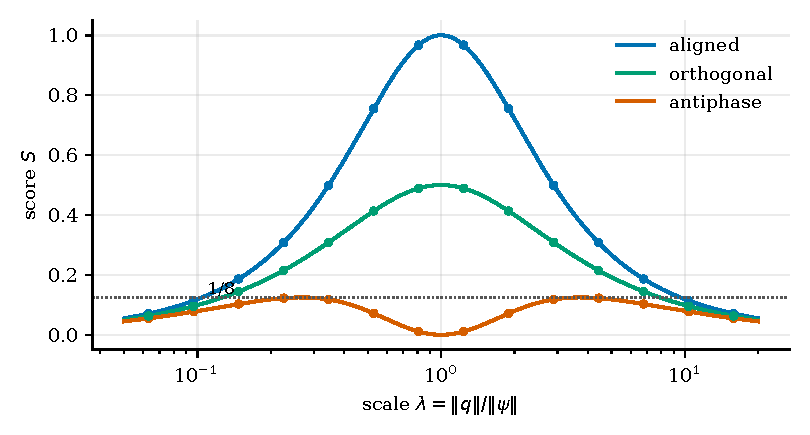
\includegraphics[width=0.85\textwidth]{figs/score_scale}
\caption{Resonance score as a function of the query scale $\lambda$ for an aligned, orthogonal and antiphase query. Curves are the closed form \eqref{eq:Aclosed}; points are the score computed from its definition on random vectors in $\C^8$. The dotted line marks the maximum $1/8$ of the antiphase curve. Computed by the script \texttt{figs.py} with seed 8; an illustration of the stated analytic result and not an evaluation of the architecture.}\label{fig:score}
\end{figure}

\chapter{Phase Transformations and Semantic Operators}\label{ch:operators}

The wave-based proposal names four semantic operators and applies them to base terms. Negation, written NEG, is described as aligning a pattern with antiphased opposites. A controlled phase shift, SHIFT+, is described as producing stable offset clusters. Two amplitude operators, INT\_UP and INT\_DOWN, are described as producing amplitude-driven zones \cite{listopad2025}. The text of the source does not give formulas, phase offsets, or scaling rules for any of them, so the operators cannot be reproduced from the paper alone. The monograph therefore adopts candidate definitions, consistent with the one-line descriptions, and states exactly what each implies for the score. The definitions are a modeling choice made here and are not claimed to be the source's.

\begin{definition}[Candidate operators]\label{def:cand-ops}
For a pattern $\psi\in\Hil$, a phase offset $\delta\in(0,\pi)$, and a scale $\gamma>1$, define $\mathrm{NEG}(\psi)=e^{\iu\pi}\psi=-\psi$, $\mathrm{SHIFT}^+_\delta(\psi)=e^{\iu\delta}\psi$, $\mathrm{INT\_UP}_\gamma(\psi)=\gamma\psi$, and $\mathrm{INT\_DOWN}_\gamma(\psi)=\gamma^{-1}\psi$.
\end{definition}

All four are multiplication by a nonzero complex scalar $\lambda=\gamma e^{\iu\delta}$, and the family of such multiplications is the multiplicative group $\C^\times$ acting on $\Hil$ by scalars. The composition law $U_gU_h=U_{gh}$ required of a group action holds, and the maps are invertible isometries up to scale. The closed form of Theorem~\ref{thm:closed} then gives the score between a pattern and its image in one line.

\begin{proposition}[Score of an operator image]\label{prop:opimage}
For $\psi\ne0$ and $\lambda=\gamma e^{\iu\delta}$, $S(\psi,\lambda\psi)=\frac\rho2(1+\rho\cos\delta)$ with $\rho=2\gamma/(1+\gamma^2)$. Consequently $S(\psi,\mathrm{NEG}\,\psi)=0$, $S(\psi,\mathrm{SHIFT}^+_\delta\psi)=\frac12(1+\cos\delta)$, and $S(\psi,\mathrm{INT\_UP}_\gamma\psi)=S(\psi,\mathrm{INT\_DOWN}_\gamma\psi)=\frac\rho2(1+\rho)$ with the same $\rho$.
\end{proposition}

\begin{proof}
Here $\norm{\lambda\psi}=\gamma\norm\psi$, so $\rho=2\gamma/(1+\gamma^2)$ and $\Re\ip{\psi}{\lambda\psi}=\norm\psi^2\Re\lambda=\norm\psi^2\gamma\cos\delta$, giving $c=\cos\delta$. Substitute into \eqref{eq:closed}; the values for the four operators follow with $(\gamma,\delta)=(1,\pi),(1,\delta),(\gamma,0)$, and $(\gamma^{-1},0)$, noting $\rho(\gamma)=\rho(\gamma^{-1})$.
\end{proof}

Two consequences are worth stating. First, the score cannot distinguish the amplitude-raising operator from the amplitude-lowering operator with reciprocal factors when each is compared against the unmodified base pattern, since the two images are equally distant in the sense of $S$. Whether the two can be distinguished at all depends on the presence of a reference scale elsewhere in the store, which is a property of the encoder and not of $S$. Second, because every candidate operator is a complex scalar, each acts identically on every coordinate pair of the realified space, as a rotation by $\delta$ combined with a scaling by $\gamma$ in each two-dimensional block. This is a one-parameter-pair family inside the real-linear maps of $\R^{2n}$, and a real-valued model that is allowed a single shared rotation-scaling block can represent every one of these operators exactly.

The semantic status of negation requires a separate argument, because the equation $\mathrm{NEG}(\psi)=-\psi$ is a mathematical convenience and not an analysis of negation. Four distinct things have been called negation in the literature on semantics and retrieval. A phase rotation by $\pi$ is an involution, $\mathrm{NEG}\circ\mathrm{NEG}=\mathrm{id}$, which agrees with the classical law that double negation returns the proposition. It is also a linear isometry, which means it maps antonyms to a set of patterns determined entirely by the geometry of the original ones: whatever is close to $\psi$ is sent to something far from $\psi$ and close to $-\psi$. This conflates contrary and contradictory opposition. The contrary of hot is cold, which is a particular alternative, whereas the contradictory of hot is not-hot, which is the whole complement, including lukewarm and cold and a great many unrelated things. A single vector $-\psi$ can stand for the contrary and cannot stand for the complement, because the complement contains patterns that are mutually orthogonal and no single point is close to all of them under any inner-product score. Negation understood as set complement is therefore not a point-to-point map but a point-to-set map, and the pointwise rotation is at best a representative of one of its members. Alternatively, negation may be modeled as a context-dependent transformation in which the effect on the pattern depends on what is being negated and why, which suggests a learned operator indexed by context; or as a relation between propositions in a separate relational structure, with the vector layer holding only the proposition content. The monograph treats the choice among these as an open modeling question to be settled by the discrimination experiments of Part~IX, and it distinguishes in every case between operators that are invertible isometries, such as phase rotations, and lossy semantic operations, such as projections onto a subspace or collapse of a set of alternatives to a representative, which are idempotent and not injective.

\chapter{ResonanceDB as a Baseline Architecture}\label{ch:resonancedb}

The software implementation accompanying the wave-based proposal is called ResonanceDB. As described in the source, patterns are stored in memory-mapped binary segments as real-valued amplitude-phase pairs and converted to complex form on demand; the similarity kernel is deterministic and retrieval is an exact scan, so there is no index and no approximation, with cost $O(NL)$ for $N$ patterns of length $L$ \cite{listopad2025}. The reported configuration uses pattern lengths $L\in\{512,1024\}$, dataset sizes from $10^4$ to $5\times10^5$ patterns, and top-$k$ retrieval with $k\in\{1,10,100\}$. Execution is on a 12-core CPU at 3.6~GHz with 32~GB of memory under Java 22, cold cache, and a fixed 12-thread executor. Two backends are described, a scalar kernel used for all reported latencies and an experimental vectorized kernel that is excluded from the results. The numerical precision of the stored values is not stated. The source reports that no training is involved, since phases are supplied by the encoder or specified procedurally.

The reported latencies at $L=1024$ and $5\times10^5$ patterns, with a heap near 512~MB, are approximately 135~ms mean and 152~ms at the 95th percentile for top-1, 138~ms and 156~ms for top-10, and 145~ms and 163~ms for top-100. The source's text describes latency as scaling linearly with dataset size, while the latency table is reported at one dataset size only, so the scaling claim is not supported by the numbers presented and is treated here as a hypothesis to be tested.

A dimensional check is useful because it indicates what a faithful reproduction must control. A full scan at the reported configuration touches $5\times10^5\times1024=5.12\times10^8$ pattern coordinates. If each coordinate is stored as an amplitude and a phase in 32-bit floating point, the scan reads $5.12\times10^8\times8=4.1$ gigabytes, and a mean latency of 135~ms then corresponds to an effective read rate of about $30$~GB/s; with 64-bit values the rate doubles. These figures are conditional on the unstated precision and on the whole file being read per query, and they are offered only to show that the result is within the range where memory bandwidth, not arithmetic, is the binding constraint, which suggests that implementation overhead and mathematical retrieval cost are not easily separated in this measurement. A second consideration concerns the arithmetic. Evaluating the interference sum for amplitude-phase storage requires $\cos(\phi_1-\phi_2)$ for each coordinate, which is a transcendental evaluation when phases are continuous and a sign when phases are restricted to $\{0,\pi\}$. The source's mapping from real embeddings assigns phase $0$ to nonnegative coordinates and phase $\pi$ to negative ones. Whether the reported latency was measured on patterns with continuous phases, and whether the scalar kernel avoids the trigonometric evaluation, cannot be determined from the text, and a latency measured on binary-phase data would not transfer to dense-phase data. The reproduction protocol of Chapter~\ref{ch:repro} therefore requires latency to be reported separately for binary-phase and continuous-phase stores.

The baseline algorithm is specified here so that every later variant can be defined as a modification of it. In notation, the exact scan computes the score of the query against every stored pattern and returns the indices of the $k$ largest scores.

\begin{Verbatim}[fontsize=\small,frame=single,framesep=2mm]
function resonance_topk(store, q, k):
    Eq <- sum_x |q[x]|^2
    heap <- empty min-heap of size k
    for i in 1..N:
        psi <- store[i]                      # amplitude-phase pairs -> complex
        E   <- sum_x |psi[x]|^2
        if E + Eq == 0:  s <- 0
        else:
            ip <- sum_x Re( conj(psi[x]) * q[x] )
            s  <- (E + Eq + 2*ip) * sqrt(E*Eq) / (E + Eq)^2
        push (s, i) onto heap, keeping the k largest
    return heap sorted descending
\end{Verbatim}

Two separations are made explicit in every later comparison. Mathematical retrieval cost is the count of arithmetic operations and memory reads that the algorithm requires on an idealized machine, here $\Theta(NL)$ reads and multiply-accumulate operations for the exact scan, and implementation overhead is everything else: input and output, memory mapping, thread scheduling, garbage collection, and conversion between storage and compute formats. Approximate indexing changes the first and can change the second in either direction, and an approximate method must be compared with the exact one at matched recall and not at matched latency alone. The energies $E=\sum_x|\psi[x]|^2$ of stored patterns can be cached at write time, which removes one of the three reductions per pattern from the inner loop, and any reported latency should state whether this was done.

\chapter{The Representational Equivalence Problem}\label{ch:equiv}

The claim that phase-aware retrieval offers an advantage over real-valued vector retrieval admits several readings, and the first task is to decide which of them is available. A categorical claim, that complex vectors can express something that real vectors cannot, is false for the following elementary reason.

\begin{theorem}[Realification]\label{thm:realif}
Define $\iota:\C^n\to\R^{2n}$ by $\iota(z)=(\Re z,\Im z)$. Then $\iota$ is an $\R$-linear bijection with $\ip{\iota z}{\iota w}_{\R}=\Re\ip{z}{w}_{\C}$ for all $z,w$, so $\C^n\cong\R^{2n}$ as real inner-product spaces. Multiplication by $\iu$ corresponds under $\iota$ to the orthogonal matrix $J=\begin{psmallmatrix}0&-I\\ I&0\end{psmallmatrix}$, which satisfies $J^2=-I$. A real-linear map $A$ of $\R^{2n}$ is of the form $\iota\circ B\circ\iota^{-1}$ for a complex-linear map $B$ of $\C^n$ if and only if $AJ=JA$.
\end{theorem}

\begin{proof}
Linearity and bijectivity are immediate. For $z=x+\iu y$ and $w=u+\iu v$, $\overline z\,w=(xu+yv)+\iu(xv-yu)$ in each coordinate, so $\Re\ip zw=\sum_k(x_ku_k+y_kv_k)=\ip{\iota z}{\iota w}$. Multiplication by $\iu$ sends $x+\iu y$ to $-y+\iu x$, hence $(x,y)\mapsto(-y,x)=J(x,y)$, and $J^2(x,y)=(-x,-y)$. If $B$ is complex-linear then $B(\iu z)=\iu B(z)$, which reads $AJ=JA$ for $A=\iota B\iota^{-1}$. Conversely, an $\R$-linear $A$ commuting with $J$ commutes with multiplication by $\iu$ and is therefore $\C$-linear.
\end{proof}

\begin{corollary}[Dimension count for the inductive bias]\label{cor:dimcount}
The space of complex-linear maps of $\C^n$ has real dimension $2n^2$, while the space of real-linear maps of $\R^{2n}$ has real dimension $4n^2$. A complex-valued linear layer is therefore a real layer with the constraint $AJ=JA$, which halves the number of free parameters.
\end{corollary}

The relationship between the score and the realification is immediate from Corollary~\ref{cor:bounds}: since $\rho$ and $c$ are functions of norms and of the real inner product, $S(z,w)=S_{\R}(\iota z,\iota w)$ where $S_{\R}(x,y)=\frac\rho2(1+\rho\,\ip xy/(\norm x\norm y))$ is the same formula on $\R^{2n}$. Retrieval over a complex store by $S$ is retrieval over the realified store by $S_{\R}$, with identical rankings.

The comparison made in the source between resonance retrieval and cosine retrieval must therefore be read as a comparison between feature maps, norm treatment, and operators, not as one between number systems. Four candidate sources of advantage can be distinguished, and each has a different experimental signature. The first is the energy-balance factor $\rho$, which is an amplitude-sensitivity that cosine discards and which could be added to a real-valued score without changing the representation. The second is the feature map. The source's mapping from real embeddings $v$ sets $A(x)=|v(x)|$ and $\phi(x)=0$ or $\pi$ according to the sign of $v(x)$, so the complex pattern equals $v(x)$ exactly, a real vector regarded as an element of $\C^n$.
\begin{proposition}[Sign-phase patterns are real vectors]\label{prop:signphase}
If $\psi(x)=|v(x)|e^{\iu\phi(x)}$ with $\phi(x)=0$ for $v(x)\ge0$ and $\phi(x)=\pi$ otherwise, then $\psi(x)=v(x)$ for every $x$. For two such patterns $\psi_u,\psi_v$ generated from real vectors $u,v$, the phase-aware cosine equals the ordinary cosine of $u$ and $v$, and $S(\psi_u,\psi_v)=\frac\rho2(1+\rho\cos(u,v))$.
\end{proposition}
\begin{proof}
For $v(x)\ge0$, $|v(x)|e^{0}=v(x)$; for $v(x)<0$, $|v(x)|e^{\iu\pi}=-|v(x)|=v(x)$. The inner product of two real-valued complex vectors is their real inner product, so $c=\cos(u,v)$.
\end{proof}
On data generated this way, the only difference between $S$ and cosine is the balance factor $\rho$, and for unit-norm embeddings there is no difference at all in ranking. Any measured advantage of resonance over cosine on such data must come either from $\rho$ acting on unequal norms or from the operators, which are the transformations that introduce phases other than $0$ and $\pi$. The third source is the family of operators, which as shown in Chapter~\ref{ch:operators} are complex scalars and so are a structured, low-dimensional subfamily of real-linear maps. A cosine baseline applied to the original real vectors cannot represent a phase offset that the real vectors do not contain, but a baseline applied to the realified vectors can, so a comparison that feeds the baseline only the original embeddings of the base terms and the complex model the operator-transformed patterns is a comparison of information supplied, not of retrieval rules. The fourth source is numerical organization and learning dynamics: the shared structure of complex arithmetic can improve optimization or conditioning when parameters are learned, which is the argument advanced in the literature on complex-valued neural networks \cite{trabelsi2018}, and which cannot arise for a retrieval rule without training.

\begin{theorem}[Matched-baseline principle]\label{thm:matched}
Let $\mathcal D$ be a dataset of complex patterns and queries and let any retrieval task be defined by the set of rankings produced by $S$. Then the realified dataset $\iota(\mathcal D)$ with the score $S_{\R}$ produces identical rankings. Consequently, a statement that resonance retrieval outperforms a real-valued method on $\mathcal D$ is equivalent to a statement that $S_{\R}$ on $\R^{2n}$ outperforms that method on $\iota(\mathcal D)$, and no property of complex numbers is involved beyond the construction of $\mathcal D$.
\end{theorem}

The protocol consequence is a requirement of matched capacity. A complex pattern of length $L$ carries $2L$ real degrees of freedom, so the real-valued baselines in Part~IX are of dimension $2L$ and are given the same encoder outputs, together with versions given only the original embeddings, so that the contribution of the operator-generated phases can be separated from the contribution of the retrieval rule. This chapter is the place where the monograph forecloses the claim of intrinsic mathematical superiority of complex embeddings as a premise. What remains possible is that the inductive bias of a structured operator family, the numerical behavior under learning, or the interpretability of phase as a relational variable provides practical advantages, and those are empirical hypotheses to be tested against matched baselines.

\part{Distributed Oscillatory Memory}

\chapter{Empirical Foundations of Macroscale Resonance}\label{ch:cabral}

The empirical motivation for treating distributed temporal coordination as a candidate substrate of memory comes from the study of Cabral, Fernandes, and Shemesh, which recorded functional magnetic resonance imaging from rat brains at a temporal resolution far finer than is customary and analyzed the resulting signals as superpositions of oscillatory modes \cite{cabral2023}. The design, as reported in the published article, was as follows. Six genetically similar female rats were each scanned twice in each of three conditions, giving twelve scans per condition, with ten-minute scans acquired at 9.4 tesla with a temporal resolution of 38 milliseconds, a sampling rate of $26.3$ Hz. The three conditions were defined by isoflurane concentration on a background of medetomidine sedation: none, which the authors call sedation, one percent, called light anesthesia, and three percent, called deep anesthesia. Signals from about fourteen hundred brain voxels in a coronal slice were band-pass filtered below $0.3$ Hz, and scans of a post-mortem rat served as a baseline against which power and component variance were judged. Principal component analysis of the covariance of the filtered signals yielded, under sedation, ten components above the post-mortem baseline whose spatial patterns showed fixed phase relationships across distinct cortical and subcortical subsystems, varying gradually and symmetrically across space, with regions oscillating in phase or in antiphase with each other, which the authors describe as characteristic of standing waves. The temporal signatures of these components, the time courses of their amplitudes, showed transient oscillations with fluctuating amplitude, and the recorded signals could be reconstructed as the linear superposition of the ten components scaled by their temporal signatures. Power extended up to about $0.3$ Hz, peaked between $0.20$ and $0.25$ Hz in cortical voxels under medetomidine and between $0.10$ and $0.15$ Hz in the striatum, and was modulated by anesthetic level. With one percent isoflurane only six components remained above baseline, with altered spatial configuration, shorter-lived oscillations, and power peaking at lower frequencies, and at three percent the variance above baseline was captured by a single component in which cortex and striatum moved together in phase at very low frequency, consistent with the authors' statement that only global aperiodic fluctuations remain under deep anesthesia. The resonance quality factor of the oscillations, which counts the cycles before the autocorrelation decays to $1/e$, was highest under medetomidine and decreased with isoflurane. An extension to a whole-brain acquisition with lower temporal resolution, repetition time $350$ ms across twelve slices in three rats, observed oscillations with overlapping phase relationships.

The authors interpret the findings with a mechanistic model in which the spatial modes are damped resonators operating in the subcritical range of a Hopf bifurcation and driven by background noise, the stochastic resonance of standing waves, whose superposition reproduces the sliding-window correlation structure of long-range functional connectivity. This regime is relevant to the specification below, because it is a damped, noise-driven regime in which the uniform state is stable and oscillations are transient responses, and not the self-sustained regime in which a continuum oscillator model would oscillate autonomously. The distinction is taken up in Chapter~\ref{ch:cgl}.

The observations are strong evidence for one claim and no evidence for several that are adjacent to it. They support the statement that spontaneous activity measured by fMRI in sedated rats is well described by a small repertoire of spatial patterns whose amplitudes oscillate transiently, with phase relationships that are stable within a condition and that depend on the sedative state. They do not establish that those patterns carry information from one region to another, which is a claim about causal transmission that requires interventions or directed measures the study does not provide. They do not establish a binding mechanism, which would require showing that the phase relationships select and group the content represented in the participating regions. They do not establish a role in memory: the recordings were made at rest, under sedation or anesthesia, in six animals, and no encoding or recall of any episode was involved. The authors themselves note that the study did not attempt to separate neural activity from neurovascular coupling. They observe that the temporal signatures do not follow the canonical hemodynamic response, that the frequencies lie above the range typically associated with the blood-oxygenation-level-dependent signal and below cardiac and respiratory rhythms, and that earlier work found coherence between local field potentials and fMRI in this range, and they conclude that a more direct neuronal contribution cannot be excluded. The relationship of these rhythms of a few tenths of a hertz to the theta and gamma rhythms usually invoked in models of hippocampal and cortical memory \cite{buzsaki2006,lisman2013}, which are more than an order of magnitude and about two orders of magnitude faster respectively, is therefore an open empirical question and not an identification. The components obtained by principal component analysis are, finally, defined by variance and orthogonality, which are properties of the method, so the interpretation of each component as a physical standing wave needs the additional tests discussed in Chapter~\ref{ch:spectral}, some of which the authors carry out through the post-mortem control and the comparison with spatially randomized patterns.

For the purposes of this monograph the study is treated as motivation of a modeling stance: macroscale activity can be organized by a small number of coordinated oscillating patterns whose phase relationships are stable and condition-dependent, and the number, frequency, and damping of the modes are state-dependent quantities. The stance suggests that a memory architecture should be allowed to use phase coordination across distributed components, and it identifies the quantities a model should expose to experiment, namely mode counts, mode frequencies, quality factors, and phase relationships, as functions of a state variable analogous to anesthetic depth. It does not constrain the mechanism by which such coordination would subserve recollection, and every architectural claim that goes beyond the stance is labeled in Chapter~\ref{ch:explains} as a hypothesis.

\chapter{Spectral Decomposition of Distributed Activity}\label{ch:spectral}

Let a distributed field be given on a finite index set $\mathcal X$ of locations by
\begin{equation}\label{eq:modes}
\Psi(x,t)=\sum_{k=1}^{K}a_k(t)\,\varphi_k(x),
\end{equation}
where the $\varphi_k$ are spatial modes and the $a_k$ are time-dependent coefficients. Which modes to use and how to estimate them are separate questions with separate answers. Laplacian eigenmodes are obtained from a graph or mesh on $\mathcal X$ with symmetric nonnegative weights $W$, degree matrix $D$, and Laplacian $L=D-W$. The matrix $L$ is symmetric positive semidefinite and has an orthonormal eigenbasis $L\varphi_k=\lambda_k\varphi_k$ with $0=\lambda_1\le\lambda_2\le\cdots$, and the graph Fourier transform of a signal $f$ on $\mathcal X$ is the vector of coefficients $\hat f_k=\ip{\varphi_k}{f}$. A wave equation $\partial_t^2\Psi=-c^2L\Psi$ on the graph has the standing-wave solutions $\Psi(x,t)=\varphi_k(x)\cos(c\sqrt{\lambda_k}\,t+\alpha)$, each with the fixed spatial profile of an eigenmode and angular frequency $c\sqrt{\lambda_k}$, so geometry alone supplies a family of candidate resonant modes whose frequencies are determined by the spectrum of the connectivity. Principal component analysis, in contrast, chooses spatial modes that maximize explained variance of the observed data, with no reference to a generative dynamics. Dynamic mode decomposition fits a linear propagator $x_{t+1}\approx Ax_t$ to the data and uses the eigenpairs $(\mu_j,\phi_j)$ of $A$, with $\mu_j=e^{(\sigma_j+\iu\omega_j)\Delta t}$, so that the growth rate $\sigma_j$ and the angular frequency $\omega_j$ of each mode are read directly from the eigenvalue and the spatial structure, including its phase map, from the eigenvector.

The distinction that matters for the use of the word oscillatory is the one between standing and traveling spatial organization.

\begin{proposition}[Standing versus traveling modes]\label{prop:standing}
Let $\phi=u+\iu v\in\C^N$ and $x(t)=\Re(\phi\,e^{\iu\omega t})=u\cos\omega t-v\sin\omega t$. Then $x(t)$ is a standing wave, meaning that $x(t)$ lies on a fixed line through the origin for all $t$, if and only if $\phi=e^{\iu\alpha}w$ for a real vector $w$ and a real angle $\alpha$, equivalently if and only if the phase differences $\arg\phi_j-\arg\phi_k$ lie in $\{0,\pi\}$ modulo $2\pi$ for all $j,k$ at which both are nonzero. If $u$ and $v$ are linearly independent, $x(t)$ traverses an ellipse in the plane they span and the spatial pattern changes shape over the period.
\end{proposition}

\begin{proof}
If $\phi=e^{\iu\alpha}w$ then $x(t)=w\cos(\omega t+\alpha)$, which lies on the line through $w$. Conversely, if $x(t)$ stays on a line for all $t$ then $u$ and $v$ are linearly dependent, so $v=\kappa u$ or $u=0$, and then $\phi=u(1+\iu\kappa)=\sqrt{1+\kappa^2}\,e^{\iu\arctan\kappa}u$, or $\phi=\iu v$, each of the stated form. The phase-difference statement holds because $\phi_j/\phi_k=w_j/w_k$ is real. When $u,v$ are independent, $x(t)$ is a nondegenerate ellipse.
\end{proof}

A fixed phase relationship across distant locations that is either zero or $\pi$, as reported for the modes of the rat study, is therefore exactly the signature of a standing wave in this sense, and a traveling wave requires a phase map that varies continuously across locations. A principal component pair in quadrature is the typical PCA signature of a traveling wave, since a single traveling wave occupies two components with equal variance and a quarter-period offset.

The legitimacy of calling a spatial mode an oscillatory mode requires conditions beyond the existence of the decomposition. Principal components of any stationary random process with a spectrum concentrated near a frequency will show peaked power spectra, so a spectral peak in a component is not by itself evidence of a generating oscillator. The conditions adopted here are four. The mode must correspond to a complex-conjugate pair of eigenvalues of a fitted propagator with $|\mu|$ close to one, and with $\omega$ separated from its neighbors in the spectrum by more than the estimation error. The mode must be reproducible across disjoint data segments within a condition. The spectral peak must exceed that of surrogate data that preserve the second-order statistics of the original, for example the covariance matrix and the power spectrum of each channel, while randomizing the cross-channel phase relationships. And the spatial phase map must conform to the standing-wave criterion of Proposition~\ref{prop:standing} within estimation error, or be explicitly reported as traveling. Only modes passing these tests are used in Mem8 as oscillatory modes, and modes failing them are used, if at all, as statistical components.

\chapter{Coupled Oscillators and Phase Synchronization}\label{ch:kuramoto}

A minimal model of distributed phase coordination assigns a phase $\theta_i$ to each of $N$ oscillators and couples them by a sinusoidal interaction,
\begin{equation}\label{eq:kuramoto}
\dot\theta_i=\omega_i+\sum_jK_{ij}\sin(\theta_j-\theta_i-\delta_{ij})+u_i(t),
\end{equation}
where $\omega_i$ is a natural frequency, $K_{ij}$ a coupling strength, $\delta_{ij}$ a phase lag, and $u_i$ an external drive. For the case of identical natural frequencies, symmetric coupling $K_{ij}=K_{ji}$, no lag, and no drive, the model is a gradient system, and its behavior is governed by a potential.

\begin{theorem}[Gradient structure of the Kuramoto system]\label{thm:kuramoto-grad}
Let $\omega_i\equiv\omega$, $\delta_{ij}=0$, $u\equiv0$, and $K$ symmetric. In the rotating frame $\vartheta_i=\theta_i-\omega t$, system \eqref{eq:kuramoto} is $\dot\vartheta=-\nabla V(\vartheta)$ with
\begin{equation}\label{eq:V}
V(\vartheta)=-\frac12\sum_{i,j}K_{ij}\cos(\vartheta_j-\vartheta_i).
\end{equation}
Consequently $V$ is nonincreasing along trajectories, with $\dot V=-\sum_i\dot\vartheta_i^2$, every trajectory converges to the set of critical points of $V$, and, since $V$ is real-analytic, to a single critical point. For the explicit Euler discretization $\vartheta^{k+1}=\vartheta^k-\Delta t\,\nabla V(\vartheta^k)$, $V$ is nonincreasing whenever $\Delta t<1/\max_i\sum_j|K_{ij}|$.
\end{theorem}

\begin{proof}
Differentiating, $\partial V/\partial\vartheta_i=-\sum_jK_{ij}\sin(\vartheta_j-\vartheta_i)$, using the symmetry of $K$ to combine the two terms in which $\vartheta_i$ appears. Hence $\dot\vartheta_i=-\partial V/\partial\vartheta_i$ and $\dot V=\sum_i(\partial V/\partial\vartheta_i)\dot\vartheta_i=-\sum_i\dot\vartheta_i^2\le0$. The state space is a torus, hence compact, so the omega-limit set is nonempty and consists of critical points by LaSalle's principle, and convergence to a single point follows from the \L ojasiewicz gradient inequality for analytic potentials. For the discretization, the Hessian of $V$ has entries bounded by Gershgorin's theorem, giving $\norm{\nabla^2V}\le2\max_i\sum_j|K_{ij}|=:\Lambda$, so $\nabla V$ is $\Lambda$-Lipschitz, and the descent lemma gives $V(\vartheta^{k+1})\le V(\vartheta^k)-\Delta t(1-\Delta t\Lambda/2)\norm{\nabla V(\vartheta^k)}^2$, which is a decrease for $\Delta t<2/\Lambda=1/\max_i\sum_j|K_{ij}|$.
\end{proof}

The theorem is the structural basis for the phase block of the minimal model in Appendix~\ref{app:minimal}, whose update is exactly the Euler step above with zero natural-frequency spread. A deterministic check on a random symmetric coupling matrix with $N=30$ oscillators and a step $0.9$ times the bound found $V$ nonincreasing at every one of $400$ steps and the order parameter equal to one to numerical precision at the end (Appendix~\ref{app:minimal}); this checks the statement and does not test any memory property.

Synchronization is not automatically beneficial. The all-to-all case with identical frequencies and uniform positive coupling $K_{ij}=K/N$ is the extreme: it is known that the fully synchronized state is the only stable equilibrium and that the set of initial conditions not converging to it has measure zero \cite{kuramoto1984,strogatz2000,acebron2005,watanabe1994}. In that regime the final phase pattern is the same for every generic initial pattern, so the map from initial relative phases to final relative phases carries no information about the initial pattern, and any code that stores differences among traces in the relative phases of the oscillators is erased. Excess global coupling therefore reduces selectivity, because it collapses the very distinctions the phases were meant to carry, and it increases interference, because a single global phase pattern is shared by every trace read through it. The opposite extreme, no coupling, leaves the phases independent and provides no coordination. The useful regime lies between: structured coupling $K_{ij}$ that is strong within coherence clusters and weak between them, so that the dynamics has several stable or metastable cluster states, each of which can serve as a context for a different subset of traces. Metastability, meaning the persistence of one cluster configuration for a long time followed by a transition to another, arises in the presence of heterogeneity of natural frequencies, delays, or noise, and the transitions between cluster states are the mechanism by which the system can move among dynamically accessible memory states. The monograph measures cluster structure by order parameters of subsets, $R_{\mathcal S}=|\frac1{|\mathcal S|}\sum_{i\in\mathcal S}e^{\iu\theta_i}|$, and by pairwise phase-locking values between oscillators.

\chapter{Oscillatory Modes as a Computational Substrate}\label{ch:cgl}

A continuum model of coordinated oscillation is supplied by the complex Ginzburg--Landau equation, written here with a drive $I$ as
\begin{equation}\label{eq:cgl}
\partial_t\Psi=(D+\iu\Omega)\Delta\Psi+(\alpha+\iu\omega)\Psi-(\beta+\iu\chi)|\Psi|^2\Psi+I(x,t).
\end{equation}
The equation is treated as a proposed Mem8 model and not as an equation established by the neuroscience; its coefficients are free parameters of the specification, and the study discussed in Chapter~\ref{ch:cabral} gives no basis for assigning them. The equation is the normal form near a Hopf bifurcation of a spatially extended medium \cite{aranson2002}, which is the reason it is a natural candidate substrate: it is the generic description of a distributed system of weakly nonlinear oscillators with diffusive coupling.

Two regimes of \eqref{eq:cgl} need to be kept apart because the empirical study fixes only one of them. For $\alpha>0$ the uniform state is unstable and the medium oscillates autonomously, which is the supercritical regime treated in Proposition~\ref{prop:planewave}. For $\alpha<0$ the uniform state is stable, the linearization about it has damped oscillatory modes with decay rates set by $\alpha-Dk^2$ and frequencies set by $\omega-\Omega k^2$, and oscillations appear only as transient responses to a drive $I$ or to noise, with a quality factor that grows as $\alpha\to0^-$. The model of Cabral and colleagues is in the second regime, a subcritical range of a Hopf bifurcation with noise-driven resonance \cite{cabral2023}, so the supercritical regime is a design choice of Mem8 for which the study offers no support, while the damped regime is the one in which a cue can be treated as a resonant drive and the reconstruction as the ringing of the mode that the cue excites. Both are carried through the specification, and the experiments of Chapter~\ref{ch:ablation} include the damped regime as a baseline.

Four features of its solution set bear on memory. The first is the family of plane-wave solutions.

\begin{proposition}[Plane waves]\label{prop:planewave}
For $I\equiv0$, $D>0$, and $\beta>0$, equation \eqref{eq:cgl} has the solutions $\Psi(x,t)=A\,e^{\iu(k\cdot x-\nu t)}$ with
\begin{equation}
A^2=\frac{\alpha-Dk^2}{\beta},\qquad \nu=\Omega k^2-\omega+\chi A^2,
\end{equation}
which exist when $Dk^2<\alpha$. The case $k=0$ is a spatially uniform oscillation with $A^2=\alpha/\beta$.
\end{proposition}

\begin{proof}
For this ansatz $\Delta\Psi=-k^2\Psi$ and $|\Psi|^2=A^2$. Substituting, the left side is $-\iu\nu\Psi$ and the right side is $[-(D+\iu\Omega)k^2+(\alpha+\iu\omega)-(\beta+\iu\chi)A^2]\Psi$. The real part gives $0=-Dk^2+\alpha-\beta A^2$, and the imaginary part gives $-\nu=-\Omega k^2+\omega-\chi A^2$.
\end{proof}

The second feature is stability. After rescaling, the uniform oscillation is stable to long-wavelength perturbations when $1+(\Omega/D)(\chi/\beta)>0$, the Benjamin--Feir--Newell criterion \cite{aranson2002}; when the criterion fails the uniform state gives way to phase turbulence or to defect-mediated turbulence, which would correspond to unstable reconstruction. The third is the structure of the non-oscillatory subcase. When $\Omega=\chi=\omega=0$ and $I$ is time-independent, equation \eqref{eq:cgl} is the gradient flow $\partial_t\Psi=-\delta\mathcal F/\delta\overline\Psi$ of the energy
\begin{equation}\label{eq:GLenergy}
\mathcal F[\Psi]=\int\Bigl(D|\nabla\Psi|^2-\alpha|\Psi|^2+\tfrac\beta2|\Psi|^4-\bigl(\overline I\Psi+I\overline\Psi\bigr)\Bigr)dx,
\end{equation}
whose local minima are stationary attractors, so the non-oscillatory medium behaves as an energy-minimizing associative memory of Hopfield type, with fixed points playing the role of stored patterns and the drive $I$ playing the role of a cue. The oscillatory terms $\Omega,\chi,\omega$ are the non-gradient terms: they are what allows propagating waves, limit cycles, and phase-coded states, and they are also what removes the guarantee that the dynamics settles. Whether these terms improve reconstruction under matched resources is exactly the question posed by the ablation experiments, and the formal separation just given makes the experiment well posed, since the nonoscillatory implementation required in Chapter~\ref{ch:oscengine} is the gradient subcase. The fourth feature concerns localized solutions and boundary conditions: with a spatially localized drive the medium supports localized structures, which would represent individual traces, and the choice of boundary condition, periodic, no-flux, or absorbing, determines which modes are admissible in the way that the geometry determines Laplacian eigenmodes in Chapter~\ref{ch:spectral}. Mode competition arises when two or more modes have positive growth rates and nonlinear saturation couples them, so that the amplitude of one suppresses the others; this is the continuum analogue of the softmax selection used in the discrete architecture.

\chapter{Temporal Binding and Phase-Coded Associations}\label{ch:binding}

A memory of an episode requires that items encountered at different times be associated in a way that preserves what is needed about their temporal relationship. Four relationships need to be distinguished because they are routinely run together. Temporal order is the relation $t_a<t_b$. Simultaneity is $|t_a-t_b|<\epsilon$ for a resolution $\epsilon$. Causal dependence is a relation of intervention, in which the occurrence of $a$ changes the occurrence or character of $b$. Mere coactivation is that $a$ and $b$ were represented at the same time in the system, for any reason. The first two are functions of timestamps, whereas the third and fourth are not, and the difference has a precise consequence: no encoding that depends only on timestamps can distinguish two histories that differ only in their causal structure. Two histories in which $a$ causes $b$ and in which a common cause produces both at the same times have identical timestamps, so by the sufficiency criterion of Chapter~\ref{ch:ident} a timing-only memory cannot support the recollection function that returns the causal structure.

Phase offers a way to encode temporal order and interval. Associate with each item a phase variable that advances at a carrier angular frequency $\omega$, and record at encoding the phase of the item. The phase difference between two items encoded at times $t_a$ and $t_b$ is $\omega(t_b-t_a)$ modulo $2\pi$, so the lag is recovered only modulo the period $T=2\pi/\omega$: a single frequency yields an aliased measurement of lag. The aliasing is resolved by a bank of frequencies.

\begin{proposition}[Multifrequency phase code]\label{prop:crt}
Let lags be integers $\ell\in\{0,\dots,L-1\}$ in units of a time step, and let $T_1,\dots,T_K$ be pairwise coprime integer periods with $\prod_kT_k\ge L$. The phase differences $\omega_k\ell\bmod 2\pi$ with $\omega_k=2\pi/T_k$ determine $\ell$ uniquely. Conversely, for any set of periods whose least common multiple is smaller than $L$, two distinct lags yield identical phase codes.
\end{proposition}

\begin{proof}
The phase difference at frequency $\omega_k$ determines $\ell\bmod T_k$. By the Chinese remainder theorem the residues $\ell\bmod T_k$ for pairwise coprime moduli determine $\ell$ modulo $\prod_kT_k$, hence uniquely in $\{0,\dots,L-1\}$. If $\mathrm{lcm}(T_1,\dots,T_K)=\Lambda<L$, then lags $0$ and $\Lambda$ both lie in $\{0,\dots,L-1\}$ and agree modulo every $T_k$.
\end{proof}

Static positional encodings in sequence models, which use sines and cosines at a geometric ladder of frequencies \cite{vaswani2017}, are phase codes of exactly this kind, assigned by the position index and not generated by dynamics. This observation fixes the right test for whether phase carries information beyond a static positional encoding. A memory in which the phases are produced by interaction of the oscillators with the input history, and in which retrieval is read from the relative phases, must be compared with a memory that receives the same positional codes as inputs. Two controls are specified. A phase-shuffle control randomizes the assignment of phases to events while preserving their marginal distribution; if sequence reconstruction is unchanged, phase was not being used. A frozen-phase control fixes the oscillator phases to their initial values; if performance is unchanged, the dynamics were not contributing. These are the controls on which the ablation program of Chapter~\ref{ch:ablation} is based.

The reconstruction of an ordered sequence from such a code proceeds by reading relative phases of the stored items at the carrier frequencies and sorting by the decoded lag. The decoded lag error under phase noise of standard deviation $\sigma_k$ at frequency $\omega_k$ is of order $\sigma_k/\omega_k$ for the lowest frequency that resolves the coarse order, and the highest frequency in the bank sets the fine resolution but is the most sensitive to noise in the same ratio, which gives the standard coarse-to-fine tradeoff of residue-number codes. The experimental protocol of Chapter~\ref{ch:sequence} reports reconstruction error as a function of phase noise for this reason.

\part{Ecphoric Reconstruction}

\chapter{The Ecphoric Interaction Operator}\label{ch:ecphoric}

Recall is defined in this monograph as a conditional dynamical process and not as a ranking. Given a cue $c_t$, persistent memory $M_t$, a context $Z_t$, and the current field and phase state $\Psi_t$, the reconstruction is
\begin{equation}\label{eq:ecphoric}
r_t=\Eph(c_t,M_t,Z_t,\Psi_t),
\end{equation}
where $\Eph$ is realized as the terminal state of a reconstruction trajectory $r^{(0)},r^{(1)},\dots$ generated by an iteration $r^{(k+1)}=\mathcal T(r^{(k)},c_t,M_t,Z_t,\Theta^{(k)})$, with $\Eph$ the limit when it exists and the stopped iterate $r^{(K)}$ under a budget otherwise. The explicit trajectory, as opposed to a single ranking operation, has three uses. It makes the dependence on the dynamical state, the phases in particular, an object of analysis instead of a hidden implementation detail. It allows the intermediate states to be inspected, which is how false attractors and premature convergence are diagnosed. And it allows the cost of recollection to be accounted for as the number of steps and the work per step, which is the quantity that Chapter~\ref{ch:amortized} trades against accuracy.

The first question is under what conditions a partial cue initiates convergence toward the historically associated state. Let $x^\star$ denote the target, the organization that the trace was formed to preserve, and suppose that for a fixed cue the iteration is a self-map $F_c(\cdot)=\mathcal T(\cdot,c,M,Z,\Theta)$ of a complete metric space with Lipschitz constant $\lambda<1$ in its first argument. Then there is a unique fixed point $r^\star(c)$ and geometric convergence, and two statements bear on the target.

\begin{theorem}[Convergence to a cue-determined state and its distance from the target]\label{thm:converge}
Let $F_c$ be a $\lambda$-contraction on a complete metric space $(\mathcal R,d)$ with $\lambda<1$. Then (i) $F_c$ has a unique fixed point $r^\star(c)$ and $d(r^{(k)},r^\star)\le\frac{\lambda^k}{1-\lambda}d(r^{(1)},r^{(0)})$ for every initialization; (ii) for every $x\in\mathcal R$, $d(x,r^\star)\le d(x,F_c(x))/(1-\lambda)$, so the distance from the fixed point to the target is bounded by the residual $d(x^\star,F_c(x^\star))$ of the target under the cue-driven map; and (iii) if $c\mapsto F_c(r)$ is $L_c$-Lipschitz uniformly in $r$, then $d(r^\star(c),r^\star(c'))\le\frac{L_c}{1-\lambda}\,d(c,c')$.
\end{theorem}

\begin{proof}
Part (i) is the Banach fixed-point theorem with its standard a priori estimate. For (ii), $d(x,r^\star)\le d(x,F(x))+d(F(x),F(r^\star))\le d(x,F(x))+\lambda d(x,r^\star)$ and rearrangement gives the bound. For (iii), $d(r^\star(c),r^\star(c'))=d(F_c(r^\star(c)),F_{c'}(r^\star(c')))\le d(F_c(r^\star(c)),F_{c'}(r^\star(c)))+d(F_{c'}(r^\star(c)),F_{c'}(r^\star(c')))\le L_cd(c,c')+\lambda d(r^\star(c),r^\star(c'))$.
\end{proof}

Part (ii) is the precise sense in which a cue initiates convergence toward an historically associated state: the cue-driven map must have the target as an approximate fixed point, with residual small relative to $1-\lambda$. Contraction ensures convergence to a fixed point and says nothing by itself about whether that fixed point is the target; the answer is entirely in the residual. Part (iii) gives the stability of recollection under cue perturbation, so that small changes of the cue produce small changes of the reconstruction, with a constant that blows up as $\lambda\to1$. A cue that is too weak or too ambiguous makes the residual large, and then the unique fixed point may lie far from the target, which is the formal content of a spurious recollection.

\chapter{Associative Completion and Attractor Geometry}\label{ch:attractor}

Completion from incomplete observations is modeled by recurrent dynamics whose fixed points are intended to coincide with stored patterns. The continuous associative memory of Ramsauer and colleagues provides the cleanest instance for the purposes of analysis \cite{ramsauer2021}. For stored unit traces $m_1,\dots,m_P$ in the realified space and an inverse temperature $\beta>0$, the update map is
\begin{equation}\label{eq:modernhop}
F(r)=\sum_{i=1}^Pw_i(r)\,m_i,\qquad w_i(r)=\frac{e^{\beta\ip{m_i}{r}}}{\sum_je^{\beta\ip{m_j}{r}}},
\end{equation}
with $\ip{\cdot}{\cdot}$ the real inner product, and its stationary points are those of the energy $\mathcal E(r)=\frac12\norm r^2-\beta^{-1}\log\sum_je^{\beta\ip{m_j}{r}}$, since $\nabla\mathcal E(r)=r-F(r)$. The relation of this update to Bayesian reconstruction is stated in Proposition~\ref{prop:map}, where it appears as a monotone algorithm for a posterior mode. The geometry of the basins can be described directly. Fixed-point, limit-cycle, and metastable attractors need to be distinguished. A fixed point corresponds to a single stable reconstruction. A limit cycle, which cannot occur for the gradient dynamics above but can occur with the non-gradient terms of Chapter~\ref{ch:cgl}, corresponds to a recollection that is a cyclically evolving state, which may represent a temporally extended episode replayed in a loop. A metastable attractor is a state in which the dynamics lingers for a long time before leaving, and corresponds to an uncommitted or blended recollection.

\begin{proposition}[Basin condition and one-step cleanup]\label{prop:basin}
Let $\norm r\le1$ and suppose that for some index $1$ one has $\ip{m_1}{r}\ge\ip{m_i}{r}+\Delta$ for all $i\ne1$. Then the weight mass outside trace $1$ satisfies $\varepsilon:=\sum_{i\ne1}w_i(r)\le(P-1)e^{-\beta\Delta}$ and
\begin{equation}
\norm{F(r)-m_1}\le2\varepsilon\le2(P-1)e^{-\beta\Delta}.
\end{equation}
Moreover, with $\mu=\max_{i\ne j}\ip{m_i}{m_j}<1$, the gap at the new state satisfies $\ip{m_1}{F(r)}-\ip{m_i}{F(r)}\ge(1-\mu)-\varepsilon(3-\mu)$ for each $i\ne1$.
\end{proposition}

\begin{proof}
Each $w_i/w_1=e^{\beta(\ip{m_i}{r}-\ip{m_1}{r})}\le e^{-\beta\Delta}$ for $i\ne1$, so $\varepsilon=\sum_{i\ne1}w_i\le(1-\varepsilon)(P-1)e^{-\beta\Delta}\le(P-1)e^{-\beta\Delta}$. Then $F(r)-m_1=\sum_{i\ne1}w_i(m_i-m_1)$ and $\norm{m_i-m_1}\le2$. For the gap, $\ip{m_1-m_i}{F(r)}=\sum_jw_j\ip{m_1-m_i}{m_j}\ge w_1(1-\mu)-\sum_{j\ne1}w_j\cdot2\ge(1-\varepsilon)(1-\mu)-2\varepsilon$, using $\ip{m_1-m_i}{m_j}\ge-2$ for the remaining terms and $\ip{m_1-m_i}{m_1}=1-\ip{m_i}{m_1}\ge1-\mu$.
\end{proof}

The proposition says that if a state is separated from competitors by a margin $\Delta$ larger than $\beta^{-1}\log(P-1)$ by a sufficient amount, then one update step places the state within an exponentially small distance of the stored trace, and the margin at the new state is of the order of $1-\mu$, which exceeds the original margin requirement. The corresponding cue thresholds follow: the cue must supply enough correlation with the target trace, relative to its correlation with all other traces, to exceed $\beta^{-1}\log\bigl((P-1)/\varepsilon\bigr)$. False attractors arise in two ways. At low $\beta$ the weights are nearly uniform for a wide range of states, $F(r)$ approaches the mean of the traces, and the dynamics has a blend state near the centroid of the store; as $\beta$ increases this state loses stability through the criterion of Theorem~\ref{thm:contract} of Chapter~\ref{ch:stability} and is replaced by metastable states between clusters of similar traces and finally by single-trace attractors. At any $\beta$, spurious mixtures of traces with high mutual overlap are stable, because a state equidistant from two near-duplicates cannot be resolved by a margin. Spurious recollections in the sense of the previous chapter are the fixed points that are not near any stored trace, and their presence as a function of $\beta$, $P$, and the overlap structure is the object of the capacity analysis in Chapter~\ref{ch:capacity}.

Figure~\ref{fig:basin} plots the observed one-step error against the margin for cues of increasing corruption. Every observation lies below the bound, which is loose by a modest factor in the exponentially small regime, and the error stays near its maximum until the margin exceeds $\beta^{-1}\ln(P-1)$.

\begin{figure}[t]
\centering
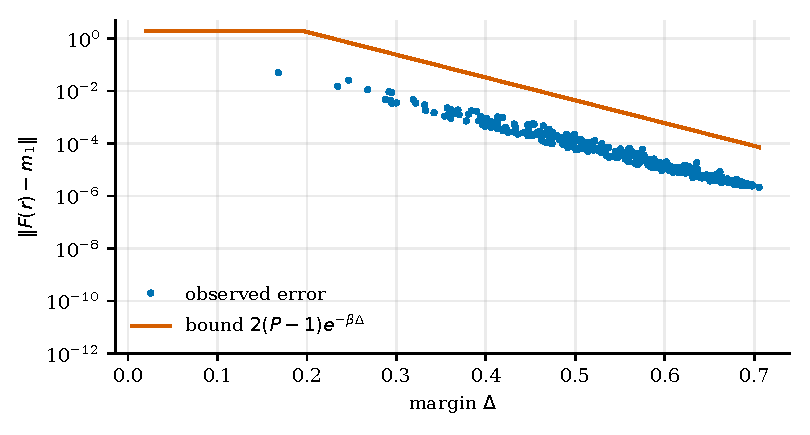
\includegraphics[width=0.85\textwidth]{figs/basin}
\caption{One-step cleanup error of the softmax update against the margin $\Delta$ for $P=50$ random unit traces in $\R^{64}$ and $\beta=20$, with the bound of Proposition~\ref{prop:basin}. Computed by the script \texttt{figs.py} with seed 8; an illustration of the stated analytic result and not an evaluation of the architecture.}\label{fig:basin}
\end{figure}

\chapter{Episodic Memory and Temporal Reinstatement}\label{ch:episodic}

Episodes are represented as trajectories and not as isolated vectors:
\begin{equation}\label{eq:episode}
e_i=\{x_i(\tau):\tau\in[t_i^-,t_i^+]\},
\end{equation}
where $x_i(\tau)$ is the organized state of the episode at internal time $\tau$. The difference between recovering what happened and recovering how it was organized in time is the difference between the content of an episode and its temporal organization. For a finite episode, content is the set or multiset of states visited, and temporal organization comprises the order in which they were visited, the intervals between them, the nesting of subepisodes, and the boundaries. Proposition~\ref{prop:nonimpl} showed that the two come apart in the encoding. They come apart in evaluation as well, which requires separate error measures. Let $x$ and $\hat x$ be a true and a reconstructed episode with item sequences $\sigma,\hat\sigma$ over a common item set. A content error is a distance between the multisets, for example the symmetric difference size. An order error is the normalized Kendall tau distance $\tau_K(\sigma,\hat\sigma)=\binom{n}{2}^{-1}\#\{\text{discordant pairs}\}$. An interval error is the root-mean-square difference of inter-item lags. A boundary error compares the sets of boundary times, for example by the F-score of boundaries matched within a tolerance. A reconstruction with zero content error and large order error is possible and is the expected failure of an encoding that stores a bag of items.

Event boundaries are defined here by a surprise criterion that follows the event-segmentation tradition in cognitive psychology \cite{zacks2007}: given a predictive model $p(x_{\tau+1}\mid x_{\le\tau})$, a boundary is placed at $\tau$ when $-\log p(x_{\tau+1}\mid x_{\le\tau})$ exceeds a threshold. Boundaries partition an episode into events and support two operations that matter for reconstruction: encoding at event level, in which each event is stored as a unit with within-event structure reconstructed from a generative model, and retrieval at event level, in which a cue first selects an event and then unfolds it. Temporal compression is the observation that recollection can proceed faster than the original episode. Let the replay map be $\tilde x(s)=x(\kappa s)$ with compression factor $\kappa>1$; for sampled trajectories this is subsampling or temporal pooling, and it reduces the cost of reconstruction by the factor $\kappa$ at the price of losing structure faster than the new sampling resolution, a loss that is bounded by the Nyquist condition on the retained structure.

Variable-resolution reconstruction is formalized by a nested family of subspaces $V_1\subseteq V_2\subseteq\cdots\subseteq V_L$ of the representation space and the corresponding orthogonal projections $\pi_\ell$. A reconstruction at level $\ell$ is $\pi_\ell\hat x$. Because the subspaces are nested, the squared error $\norm{x-\pi_\ell x}^2$ is nonincreasing in $\ell$, and the cost of reconstruction increases with $\ell$, so a coarse reconstruction at low cost can be refined as the task requires. The same family underlies the multiscale consolidation of Chapter~\ref{ch:consolidation}.

\chapter{Context-Sensitive Reconstruction}\label{ch:context}

Context is modeled as an operator acting on cues and candidate memories, so that the reconstruction under context $Z_t=z$ is
\begin{equation}\label{eq:context}
r_t=\Eph_{z}(c_t,M_t),
\end{equation}
where the operator $U_z$ acts on the cue before scoring and, in some formulations, on the stored traces as well. For a context group acting by unitary operators with $U_zU_{z'}=U_{z+z'}$, the effective score of a trace $m$ against a cue $c$ under context $z$ is $S(m,U_zc)$. This single construction accounts for four properties that are otherwise treated separately. Context-dependent accessibility arises because the score of a given trace against a given cue depends on $z$ through $U_z$. Cue ambiguity arises because the same $c$ under different contexts may match different traces. Competing interpretations arise because several $(m_i,z)$ pairs may give comparable scores. The effective retrieval landscape, the function $m\mapsto S(m,U_zc)$ over the store, changes with $z$ even though the store is unchanged.

Encoding specificity takes an exact form in the phase-context case. Let content be a unit vector $s$ and let the context be a global phase, $U_zs=e^{\iu z}s$.

\begin{proposition}[Encoding specificity as phase mismatch]\label{prop:encspec}
If a trace is stored as $m=U_{z_0}s$ and the cue is the same content presented under context $z$, $c=U_zs$, then $S(m,c)=\tfrac12\bigl(1+\cos(z-z_0)\bigr)$. The score equals one for matched context and zero for contexts differing by $\pi$, independent of the content.
\end{proposition}

\begin{proof}
Both vectors have unit norm, so by \eqref{eq:normalized} $S=\frac12(1+\Re\ip{e^{\iu z_0}s}{e^{\iu z}s})=\frac12(1+\Re e^{\iu(z-z_0)})$.
\end{proof}

The proposition formalizes the principle of Tulving and Thomson that the effectiveness of a retrieval cue depends on its overlap with the encoding context \cite{tulving1973}, with phase as the carrier of the context. Two corollaries follow from the structure of $U_z$. Because $U_z$ is invertible, the loss of accessibility caused by a context mismatch is not a loss of information: a system that can estimate the encoding context can undo the mismatch by applying $U_{z_0}U_z^{-1}$ to the cue, and the recovery of a trace by context reinstatement is exactly the application of this inverse. Second, when the context is not known, it can be marginalized or estimated: the posterior over context given the cue and the store is $p(z\mid c)\propto p(z)\sum_ie^{\beta S(m_i,U_zc)}$, and the system may either report the retrieval under the maximum a posteriori context or retain the mixture. The second option is the one required for a faithful treatment of ambiguity, since a hard assignment of context discards the information that the cue was compatible with several.

\chapter{Recollection, Familiarity, and Source Discrimination}\label{ch:source}

Recognition of familiar content and recovery of its historical context are different operations and must be distinguishable in a formal account. Let each trace carry a content part $\psi_i$ and a context-and-provenance part $\kappa_i$ (Chapter~\ref{ch:substrate}). Familiarity is a function of the content scores alone, for example $f(c)=\max_iS(\psi_i,c)$ or a smooth maximum $\beta^{-1}\log\sum_ie^{\beta S(\psi_i,c)}$. Recollection involves, in addition, the scores of the context parts, and the recollective output is not merely a number but a reconstruction with an attribution of source and context.

\begin{proposition}[Content-only familiarity cannot discriminate source]\label{prop:source}
Suppose two traces have identical content $\psi_A=\psi_B$ and different context-provenance parts $\kappa_A\ne\kappa_B$. Then any familiarity function that depends on the trace set only through the content scores takes equal values on the two traces, and no such function can assign different support to the hypotheses that the content was encountered in context $A$ or in context $B$.
\end{proposition}

\begin{proof}
A function of $\{S(\psi_i,c)\}_i$ treats traces $A$ and $B$ symmetrically because their content scores coincide for every cue $c$.
\end{proof}

Source attribution requires scoring the provenance parts, and the natural construction is a posterior over sources. With provenance labels $\nu_i$ and trace weights $w_i$ from the retrieval stage, define the attribution distribution $p(\nu\mid c)=\sum_i w_i\mathbb 1[\nu_i=\nu]$, and define source-attribution confidence as the probability mass on the most probable source, with a margin over the second. Two failure types can then be separated: content retrieval that is accurate with source misattribution, in which the content weights concentrate on traces whose content matches but whose provenance label differs from the true source because the encoding contexts were similar or because the cue carries stronger contextual overlap with the wrong source, and source attribution that is accurate for a content that is wrongly reconstructed. Provenance reconstruction, as distinct from provenance lookup, is the process of inferring the context of the original event from the stored context parts and the current state, and it is subject to all the interference effects of Chapter~\ref{ch:interference}. The consequence for architecture is that the provenance part of a trace must be a first-class component of the stored record, and that source discrimination is a test on which static content-addressable stores fail by construction, which makes it a meaningful discriminating experiment in Chapter~\ref{ch:source-exp}.

\chapter{Memory Interference and False Recollection}\label{ch:interference}

Interference is the degradation of recollection of one item by the presence of others. Four varieties are distinguished: proactive interference, in which earlier traces degrade the acquisition or retrieval of later ones; retroactive interference, in which later traces degrade earlier ones; trace competition, in which several traces compete for the same cue; and source confusion, in which the content is retrieved with the wrong attribution. In the softmax retrieval model, the effect of an additional trace on the weight of a target is exact.

\begin{proposition}[Dilution by an added trace]\label{prop:dilution}
Let a store give a target trace weight $w_t=e^{\beta s_t}/Z$ with $Z=\sum_je^{\beta s_j}$, and add a trace with score $s_n$ against the same cue. The new weight is $w_t'=w_t\,Z/(Z+e^{\beta s_n})$, and the fractional loss $1-w_t'/w_t=e^{\beta s_n}/(Z+e^{\beta s_n})$ equals the weight that the new trace itself receives.
\end{proposition}

\begin{proof}
The partition function becomes $Z'=Z+e^{\beta s_n}$ and the numerator is unchanged.
\end{proof}

The proposition shows that the interference caused by a trace is proportional to the probability mass it captures, which is largest when its score approaches or exceeds the target's, and negligible when $\beta(s_n-s_t)$ is very negative. In this model proactive and retroactive interference are arithmetically the same at retrieval: the order of storage does not enter. Distinguishing them requires an additional mechanism that depends on age or on write order, such as the amplitude decay discussed in Chapter~\ref{ch:forgetting} through the balance factor $\rho$, or a write rule that orthogonalizes a new trace against existing ones, so that the proactive and retroactive effects are caused by different parts of the architecture and are separately identifiable.

False recollection is a reconstruction that matches strongly but is historically wrong. A classical case is the production of a critical lure after studying a list of its associates \cite{roediger1995}, and a model of the effect follows from the geometry of the store.

\begin{proposition}[Centroid lure]\label{prop:lure}
Let $m_1,\dots,m_P$ be unit vectors with common pairwise real inner product $\mu\in[0,1)$, and let $g=\frac1P\sum_im_i$. Then $\norm g^2=(1+(P-1)\mu)/P$ and the normalized centroid $\hat g=g/\norm g$ satisfies $\ip{\hat g}{m_j}=\sqrt{(1+(P-1)\mu)/P}=:\kappa_P<1$ for every $j$. For a reconstruction $r=\hat g$, $S(r,\hat g)=1>S(r,m_j)=\tfrac12(1+\kappa_P)$, so the lure resonates more strongly than any presented item.
\end{proposition}

\begin{proof}
$\norm g^2=P^{-2}\bigl(P+P(P-1)\mu\bigr)$ and $\ip g{m_j}=P^{-1}(1+(P-1)\mu)$, so $\ip{\hat g}{m_j}=\ip g{m_j}/\norm g=\sqrt{(1+(P-1)\mu)/P}$, which is below one because $\mu<1$. The scores follow from \eqref{eq:normalized}.
\end{proof}

The proposition shows that a high resonance score cannot by itself certify historical support, since a composite assembled from many traces can be closer to a hypothetical item than to any actual one. The architecture therefore requires a quantity that is separate from resonance and that measures support by the ledger of Chapter~\ref{ch:provenance}.

\begin{definition}[Resonance and historical support]\label{def:support}
Let a reconstruction $r$ be given with resonance $\mathrm{res}(r)=\max_iS(m_i,r)$ against the store and let the ledger $H$ contain the inscription records. The reconstruction is $\delta$-supported if there is an inscription record $h\in H$ with $d(r,\mathrm{dec}(h))\le\delta$, where $\mathrm{dec}(h)$ is the content recorded at inscription, and is a constructed reconstruction otherwise. A recollection is reported as supported only if it is $\delta$-supported or if it is declared as a composite with the identified supporting records and their weights.
\end{definition}

With this separation the model can report a highly resonant but constructed reconstruction as such, and the evaluation in Chapter~\ref{ch:source-exp} measures the false-recollection rate as the fraction of reported-supported recollections that fail the ledger check against the ground truth of the experiment.

\part{Predictive Inference and Memory}

\chapter{Memory as Inference over Latent Causes}\label{ch:inference}

Recollection is formulated as inference under a generative model in which the past organization is a latent cause of the present cue. Let $x$ denote the latent past organization, $M$ the persistent memory, $Z$ the current context, and $c$ the cue. The recollection problem is to compute or approximate
\begin{equation}\label{eq:posterior}
p(x_{t_0}\mid c_t,M_t,Z_t)\ \propto\ p(c_t\mid x_{t_0},Z_t)\,p(x_{t_0}\mid M_t).
\end{equation}
The factor $p(x\mid M)$ is the prior over past organizations that the persistent memory induces, and the factor $p(c\mid x,Z)$ is the cue likelihood, which says how a cue is produced from the past organization under the present context. The decomposition places the contribution of memory and the contribution of evidence in separate terms and makes explicit that recollection draws on both.

The softmax retrieval rule that appears throughout the monograph is the exact Bayesian posterior mean under a simple instance of this model. Let the prior be a mixture of isotropic Gaussians centered on the stored traces, $p(x\mid M)=\sum_i\pi_i\,\mathcal N(x;m_i,\sigma_x^2I)$, and let the cue be a noisy full observation, $c=x+\xi$ with $\xi\sim\mathcal N(0,\sigma_c^2I)$, all in the realified space.

\begin{proposition}[Softmax readout as posterior mean]\label{prop:posteriormean}
Under this model the posterior is a mixture with weights $w_i\propto\pi_i\exp\bigl(-\norm{c-m_i}^2/(2s^2)\bigr)$, $s^2=\sigma_x^2+\sigma_c^2$, and posterior mean
\begin{equation}\label{eq:postmean}
\Ex[x\mid c]=(1-g)\sum_iw_im_i+g\,c,\qquad g=\frac{\sigma_x^2}{\sigma_x^2+\sigma_c^2}.
\end{equation}
If the traces and the cue have equal norms and the prior is uniform, then $w_i=\softmax_i(\beta\ip{c}{m_i})$ with $\beta=1/s^2$, the weight rule of \eqref{eq:modernhop}.
\end{proposition}

\begin{proof}
Marginalizing $x$ within component $i$, the cue is distributed as $\mathcal N(m_i,s^2I)$, which gives the mixture weights by Bayes' rule. Within component $i$ the posterior of $x$ is Gaussian with mean $(\sigma_c^2m_i+\sigma_x^2c)/s^2=(1-g)m_i+gc$. Averaging over components gives \eqref{eq:postmean}. For equal norms, $\norm{c-m_i}^2=\norm c^2+\norm{m_i}^2-2\ip c{m_i}$, and the terms that do not depend on $i$ cancel in the normalization, leaving $w_i\propto\exp(\ip c{m_i}/s^2)$.
\end{proof}

The resemblance between this expression and the recurrent relaxation step needs care, because two different operators are involved. The posterior mean \eqref{eq:postmean} is a one-shot reconstruction operator: its weights are evaluated at the cue, with inverse temperature $\beta_c=1/(\sigma_x^2+\sigma_c^2)$, and the coefficient $g$ weights the observation itself, so that a precise cue ($\sigma_c\to0$) gives $g\to1$ and the reconstruction follows the cue. The relaxation step of the minimal model, $r^{(k+1)}=(1-\eta)r^{(k)}+\eta\sum_iw_i(r^{(k)})m_i$, is an iteration whose weights are evaluated at the current state and whose coefficient $\eta$ is a step size and not a reliability ratio. Both are convex combinations of a memory-weighted readout with another vector, and that is all the resemblance establishes. A formal relationship requires an objective whose stationary points the iteration computes, and such an objective exists. Take unit-norm traces, a uniform prior, and write $\beta_x=1/\sigma_x^2$ and $\mathcal E_{\beta}$ for the energy of Chapter~\ref{ch:attractor} at inverse temperature $\beta$. The negative log of the unnormalized posterior over the latent organization $x$ given the cue is, up to an additive constant,
\begin{equation}\label{eq:Jobj}
J(x)=\beta_x\,\mathcal E_{\beta_x}(x)+\frac{\norm{x-c}^2}{2\sigma_c^2},
\end{equation}
since $\log\sum_ie^{-\norm{x-m_i}^2/2\sigma_x^2}=-\tfrac12\beta_x\norm x^2+\log\sum_ie^{\beta_x\ip{m_i}{x}}+\mathrm{const}$ for unit-norm traces.

\begin{proposition}[Cue-anchored recurrence computes posterior modes]\label{prop:map}
Let $L=\beta_x+\sigma_c^{-2}$, let $g=\sigma_x^2/(\sigma_x^2+\sigma_c^2)$, and define $T(x)=(1-g)F_{\beta_x}(x)+g\,c$, where $F_{\beta_x}$ is the softmax update \eqref{eq:modernhop} at inverse temperature $\beta_x$. Then $\nabla J(x)=L\,(x-T(x))$, so the stationary points of $J$ are exactly the fixed points of $T$. For every $\eta\in(0,2)$ the damped iteration $x^{+}=(1-\eta)x+\eta\,T(x)$ satisfies
\begin{equation}
J(x^{+})\le J(x)-L\,\eta\Bigl(1-\frac\eta2\Bigr)\norm{x-T(x)}^2,
\end{equation}
so $J$ decreases along the iteration, and every limit point of the iteration is a fixed point of $T$. When $\sigma_c\to\infty$ the iteration reduces to the cue-free relaxation $x^+=(1-\eta)x+\eta F_{\beta_x}(x)$, which descends the energy $\mathcal E_{\beta_x}$.
\end{proposition}

\begin{proof}
The gradient is $\nabla J(x)=\beta_x(x-F_{\beta_x}(x))+(x-c)/\sigma_c^2$. Since $L(1-g)=\beta_x$ and $Lg=\sigma_c^{-2}$, this equals $L(x-T(x))$. For the decrease, write $J(x)=\tfrac12L\norm x^2-\ip x c/\sigma_c^2-\ell(x)+\mathrm{const}$ with $\ell(x)=\log\sum_ie^{\beta_x\ip{m_i}{x}}$, which is convex with $\nabla\ell(x)=\beta_xF_{\beta_x}(x)$. Linearizing $\ell$ at $x$ gives the majorizer $\tilde Q(y)=\tfrac12L\norm y^2-\ip yc/\sigma_c^2-\ell(x)-\ip{\beta_xF_{\beta_x}(x)}{y-x}\ge J(y)$ with equality at $y=x$. The function $\tilde Q$ is a quadratic of curvature $L$ minimized at $y=T(x)$, with $\nabla\tilde Q(x)=-L(T(x)-x)$. Along the segment $x+\eta(T(x)-x)$, $\tilde Q$ equals $\tilde Q(x)-L(\eta-\eta^2/2)\norm{T(x)-x}^2$, and $J\le\tilde Q$ with $J(x)=\tilde Q(x)$ gives the stated inequality. The function $J$ is bounded below and coercive, because $\log\sum_ie^{\beta_x\ip{m_i}{x}}\le\log P+\beta_x\norm x$. The summed decreases are therefore finite, $\norm{x-T(x)}\to0$, and continuity of $T$ shows that limit points are fixed points. The final statement is the case $L=\beta_x$, $g=0$.
\end{proof}

The proposition is the precise relationship between the two operators. The recurrent iteration is a monotone algorithm for the posterior mode, an instance of the concave--convex procedure, and in the cue-free case it is the mean-shift or expectation-maximization mode-finding iteration for the Gaussian mixture density of variance $\sigma_x^2$ \cite{carreira2000}. The posterior mean \eqref{eq:postmean} is a different object, a minimum-mean-square-error estimate evaluated at the cue with the flatter weights $\beta_c<\beta_x$. The two agree when the memory holds a single trace, since then $F\equiv m_1$ and both reduce to $(1-g)m_1+gc$, and in general they differ: the mode of a multimodal posterior is a stored trace blended with the cue, while the posterior mean is an average over modes. The monograph therefore treats them as two reconstruction operators that answer different questions, and the sharpness parameter that governs selection in the recurrent iteration is $\beta_x=\sigma_x^{-2}$, the precision of the prior around each trace, and not the total precision of the cue and trace.

Three forms of inference over time should be distinguished. Filtering estimates the present state from past observations and is the mode used in forward prediction. Smoothing estimates a past state from observations that include later ones, and recollection of an earlier episode is naturally a smoothing problem, because the cue at recall time, and what has been learned since, are evidence about the earlier state. Prediction extrapolates forward from an estimated state. Reconstruction and prediction are therefore posteriors over latent states at different times under a common generative model, which accounts for the empirical coupling between remembering the past and imagining the future without identifying the two. Amortized inference replaces the iterative computation of the posterior by a trained map $q_\phi(x\mid c,M,Z)$; the penalty is the amortization gap, the expected divergence $\Ex_c\KL(q_\phi(\cdot\mid c)\,\Vert\,p(\cdot\mid c))$ between the learned approximation and the true posterior, and Chapter~\ref{ch:amortized} treats when it is worth paying.

\chapter{Variational Ecphory}\label{ch:variational}

Let $q$ be an approximate posterior over the latent organization. The variational free energy of the recollection problem is
\begin{equation}\label{eq:vfe}
\mathcal F[q]=\Ex_q\bigl[-\log p(c,x\mid M,Z)\bigr]-H(q).
\end{equation}

\begin{proposition}[Decomposition of the free energy]\label{prop:vfe}
For every distribution $q$ with support contained in that of the posterior, $\mathcal F[q]=\KL\bigl(q\,\Vert\,p(\cdot\mid c,M,Z)\bigr)-\log p(c\mid M,Z)$. Hence $\mathcal F[q]\ge-\log p(c\mid M,Z)$ with equality if and only if $q$ is the exact posterior.
\end{proposition}

\begin{proof}
Write $p(c,x\mid M,Z)=p(x\mid c,M,Z)\,p(c\mid M,Z)$. Then $\Ex_q[-\log p(c,x)]=\Ex_q[-\log p(x\mid c)]-\log p(c)$, and $-H(q)=\Ex_q[\log q]$, so the sum is $\Ex_q[\log q-\log p(x\mid c)]-\log p(c)=\KL(q\Vert p(\cdot\mid c))-\log p(c)$. Nonnegativity of the divergence gives the inequality and its equality case.
\end{proof}

Two sources of uncertainty enter any recollection and the framework requires that they be kept apart. The first is uncertainty about the historical episode that remains even when the posterior is computed exactly, measured by the posterior entropy $H(p(\cdot\mid c,M,Z))$ and, for point estimates, by the posterior covariance. It is a property of what the memory and the cue together determine. The second is uncertainty caused by present retrieval dynamics: the system does not hold the exact posterior but a truncated or biased approximation $q_k$ after $k$ iterations, and its excess relative to the exact posterior is the inference gap $\mathcal F[q_k]-\mathcal F[p]=\KL(q_k\Vert p)\ge0$. For a point estimate $\hat x$ that is a function of the cue, the corresponding decomposition of squared error is exact.

\begin{proposition}[Irreducible and reducible error]\label{prop:error}
For any estimator $\hat x(c)$ and posterior mean $\mu(c)=\Ex[x\mid c]$, $\Ex\bigl[\norm{x-\hat x(c)}^2\mid c\bigr]=\operatorname{tr}\Cov(x\mid c)+\norm{\mu(c)-\hat x(c)}^2$. The first term does not depend on the estimator and is the irreducible uncertainty about the episode given cue and memory; the second is the reducible part attributable to the retrieval procedure.
\end{proposition}

\begin{proof}
Add and subtract $\mu(c)$ inside the norm; the cross term vanishes because $\Ex[x-\mu(c)\mid c]=0$.
\end{proof}

The monograph reports reconstruction error in this decomposed form wherever the posterior is available, so that an improvement in retrieval dynamics cannot be mistaken for a reduction in intrinsic uncertainty and a system that is confidently wrong can be distinguished from one that is appropriately uncertain.

\chapter{Precision Weighting and Resonance Selection}\label{ch:precision}

Precision-sensitive cue integration weights each source of evidence by its reliability, and the architecture contains three places where an oscillatory coherence signal could plausibly act. It could change the gain on incoming evidence, so that coherent states give more weight to the cue. It could change the selection of memory traces, so that coherence sharpens or flattens the competition among them. It could change the transition dynamics of the reconstruction process, so that coherence speeds or slows convergence. These are distinct hypotheses with different observable signatures, and the first task is to determine which of them are distinguishable at all from outcomes.

Consider unit-norm traces and several cues $c_1,\dots,c_J$ with precisions $\Pi_1,\dots,\Pi_J$, each cue observing the target with independent Gaussian noise of variance $1/\Pi_j$. By the calculation of Proposition~\ref{prop:posteriormean} extended to several cues, the trace weights are
\begin{equation}\label{eq:multicue}
w_i\ \propto\ \pi_i\exp\Bigl(\sum_{j=1}^J\Pi_j\ip{c_j}{m_i}\Bigr).
\end{equation}
A uniform gain $\gamma$ on all evidence multiplies every $\Pi_j$ by $\gamma$, and a change of the selection temperature, $\beta\mapsto\gamma\beta$, multiplies the whole exponent by $\gamma$ as well.

\begin{proposition}[Identifiability of the three loci]\label{prop:loci}
(i) A uniform gain on evidence and a change of the selection inverse temperature produce identical trace weights, and cannot be distinguished by the weights, the reconstruction at convergence, or the accuracy. (ii) They can be distinguished by cue-specific precision, because gain changes act on $\Pi_j/\Pi_{j'}$ only if the gain depends on the cue, whereas a temperature change leaves relative cue weighting fixed. (iii) A change of the relaxation coefficient $\eta$ in $r^{(k+1)}=(1-\eta)r^{(k)}+\eta\sum_iw_im_i$ leaves the fixed point unchanged and changes only the rate, with error $(1-\eta)^k\norm{r^{(0)}-r^\star}$ at step $k$.
\end{proposition}

\begin{proof}
(i) is immediate from \eqref{eq:multicue}: the exponent is scaled by $\gamma$ in both cases. For (ii), if the gain applies uniformly then $\Pi_j/\Pi_{j'}$ is unchanged, and the weight vector is a function only of the common scale and the ratios, so a uniform gain cannot be told from a temperature change; a cue-specific gain changes the ratios, which no temperature change can do. For (iii), the fixed point of $r\mapsto(1-\eta)r+\eta v$ with $v=\sum_iw_im_i$ is $v$ for every $\eta\in(0,1]$, and $r^{(k)}-v=(1-\eta)^k(r^{(0)}-v)$.
\end{proof}

The implication for empirical discrimination is a design requirement. To separate the gain and selection hypotheses the experiment must manipulate the relative reliability of two or more cues while manipulating coherence; to separate transition effects from the other two, it must record the time course of convergence in addition to the endpoint. A coherence manipulation that changes only endpoint accuracy cannot discriminate among the three, and the program in Chapter~\ref{ch:ablation} is specified to include these manipulations.

\chapter{Active Inference and Prospective Memory}\label{ch:active}

Reconstruction extends to action selection and future simulation by embedding the recollected state in a model of the future. The standard formalism, active inference, evaluates candidate policies $\pi$ by their expected free energy,
\begin{equation}\label{eq:efe}
G(\pi)=\Ex_{q(o,s\mid\pi)}\bigl[\log q(s\mid\pi)-\log p(o,s\mid\pi)\bigr]
\end{equation}
which, under a prior preference distribution $p(o)$ over outcomes, decomposes into a risk term, the divergence of predicted outcomes from preferred outcomes, and an ambiguity term, the expected uncertainty of outcomes given states \cite{friston2017,parr2022}. Remembered states enter through the predictive prior: a recollection $q(x_{t_0}\mid c,M,Z)$ informs beliefs about the present and future state through the transition model $p(s_{t+1}\mid s_t,a)$ for states that depend on the remembered organization. Remembering is not thereby identified with planning, because the two computations condition on different things. Recollection conditions on a cue about the past and on persistent memory, and its posterior \eqref{eq:posterior} contains no term for preferences or policies. Planning conditions on candidate policies and on preferences, and its posterior over policies is proportional to $\exp(-\gamma G(\pi))$. They are connected through the shared generative model and distinct in the quantities that define their objectives.

It follows that the value of a future continuation is not equivalent to the historical accuracy of a recollection, and a system optimizing one can sacrifice the other. A reconstruction biased toward outcomes that are favorable under the current preferences can have higher expected value for action selection and lower fidelity to the history, and an accurate reconstruction of a history irrelevant to the present can be of no value. Mem8 therefore keeps two separately defined objectives. The recollection objective is the variational free energy of Chapter~\ref{ch:variational}, with historical fidelity measured against the ledger, and the decision objective is the expected free energy \eqref{eq:efe} or a utility from Chapter~\ref{ch:viability}. A specification that merged them into a single scalar would make it impossible to detect the case in which fidelity has been traded for value, and the architecture rules out silent trade by treating fidelity as a constraint, not as one term of a sum, in Chapter~\ref{ch:viability}.

\chapter{Amortized Deliberation and Learned Retrieval Policies}\label{ch:amortized}

Reconstruction costs computation, and the cost is not always justified. The system faces a recurring choice among three actions when a cue arrives: to reuse a cached reconstruction produced earlier for a similar cue and context, to initiate a full ecphoric process, or to acquire further evidence before reconstructing. The distinction between costly reconstruction and cached retrieval is the memory-specific instance of a general distinction between deliberation whose cost is paid at decision time and responses amortized from earlier deliberation, with the cost spread over many uses; the same decision-theoretic structure applies whether the cached object is an intuitive judgment or a stored reconstruction, and what varies is only the price and the validity conditions.

The contraction analysis of Chapter~\ref{ch:ecphoric} supplies a principled validity condition for the cache and a principled stopping rule for the iteration.

\begin{proposition}[Cache validity radius and iteration budget]\label{prop:cache}
Let the reconstruction map be a $\lambda$-contraction with cue-Lipschitz constant $L_c$ as in Theorem~\ref{thm:converge}. A reconstruction cached for cue $c'$ is within $\varepsilon$ of the fixed point for cue $c$ whenever $d(c,c')\le\varepsilon(1-\lambda)/L_c$. Starting from any $r^{(0)}$, the iteration is within $\varepsilon$ of its fixed point after
\begin{equation}
k\ \ge\ \frac{\ln\bigl(\varepsilon(1-\lambda)/d(r^{(1)},r^{(0)})\bigr)}{\ln\lambda}
\end{equation}
steps. In the relaxation map of the minimal model with fixed weights, $\lambda=1-\eta$ and the error after $k$ steps equals $(1-\eta)^k$ times the initial error.
\end{proposition}

\begin{proof}
The first statement is part (iii) of Theorem~\ref{thm:converge} rearranged. The second solves $\lambda^kd(r^{(1)},r^{(0)})/(1-\lambda)\le\varepsilon$ for $k$, noting that $\ln\lambda<0$ reverses the inequality. The last statement is part (iii) of Proposition~\ref{prop:loci}.
\end{proof}

A policy for the choice among reuse, reconstruction, and evidence acquisition is a map from the observable state, which includes the cue, the context, the age and provenance of the cached item, and the current uncertainty, to an action. The optimal policy compares net values: reuse has cost near zero and a value reduced by the expected error at cache distance; reconstruction has cost proportional to the iteration count of Proposition~\ref{prop:cache} and a value corresponding to the residual error; evidence acquisition has the cost of the observation and a value equal to the expected reduction of posterior uncertainty, which the variational account of Chapter~\ref{ch:variational} makes computable as an expected information gain. Under a myopic value-of-computation criterion, the iteration continues while the expected decrease in loss from one more step exceeds the marginal cost of the step, and stops otherwise. A learned retrieval policy amortizes this decision as a trained classifier over the observable state, which is itself an instance of the amortized deliberation that it governs: the policy's own cost is paid once at training and spread over all later decisions, and its validity depends on the stationarity of the distribution of cues, so its failure under distribution shift is a failure mode to be tested in Chapter~\ref{ch:failure}.

\part{Persistence, Consolidation, and Transformation}

\chapter{Encoding as the Creation of Recoverable Constraints}\label{ch:encoding}

Encoding is treated here as an operation that changes the set of future states that can be recovered from partial cues, not as the deposit of a copy. A history $h$ leaves a memory state $E(h)$, and what matters about that state is the set of reconstructions it makes available under a family of cues and contexts. Recoverability must therefore be defined relative to such a family, since a trace that no admissible cue can elicit is, for practical purposes, absent, and a trace that many cues can elicit is robust.

\begin{definition}[Recoverability]\label{def:recov}
Fix a cue family $Q$, a context family $\mathcal Z_0$, a target recollection function $T:\Hist\times\Cues\to\Recs$, a tolerance $\delta\ge0$, and a metric $d$ on $\Recs$. A history $h$ is $(Q,\mathcal Z_0,\delta)$-recoverable from the memory state $m$ if
\begin{equation}
\sup_{c\in Q,\,z\in\mathcal Z_0}d\bigl(\Eph(m,c,z),T(h,c)\bigr)\le\delta.
\end{equation}
It is cue-wise recoverable at $(c,z)$ if the inequality holds at that single pair.
\end{definition}

The definition makes explicit that storage of a trace does not guarantee recollection. In the softmax memory of Chapter~\ref{ch:attractor}, a trace $m_1$ among $P$ stored traces is recoverable to within $2\varepsilon$ at a cue only if the cue gives it a margin $\Delta$ over every competitor with $\Delta\ge\beta^{-1}\log\bigl((P-1)/\varepsilon\bigr)$ (Proposition~\ref{prop:basin}), and for cues orthogonal to all traces the weights are uniform and the reconstruction is the centroid of the store, from which no individual trace can be read. Adding traces raises the required margin logarithmically in $P$, which is a precise sense in which each new encoding changes the recoverability of the old ones without altering them. Conversely, a well-chosen encoding can create recoverability that did not exist: writing a trace that links a previously inaccessible content to a cue that is commonly available enlarges the recoverable set for that content without touching the content itself. The monograph accordingly describes the encoding stage by its effect on the recoverable set, and it requires of any encoding rule a statement of the cue and context families for which it intends to create recoverability.

\chapter{Consolidation and Multiscale Memory}\label{ch:consolidation}

A single store with a single timescale cannot be both plastic enough to absorb new episodes quickly and stable enough to retain old structure without interference, and the standard resolution is a division of labor among systems with different rates, in which fast learning of specific episodes is combined with slow integration of shared structure through repeated, interleaved replay \cite{mcclelland1995}. Mem8 adopts a layered form of this division. Transient activation, the fields and phases of Part~III, lives on timescales of milliseconds to seconds and is not itself persistent. A fast store holds recent traces with high fidelity and orthogonalized, pattern-separated codes, together with the full provenance of each. A slow store holds overlapping distributed codes that capture regularities across many episodes and supports semantic completion, and it is updated by replay of traces from the fast store at a small learning rate. Episode-specific provenance remains in the ledger of Chapter~\ref{ch:provenance} and is not folded into the slow store, so that consolidation changes where a content is accessible from without changing the record of where it came from.

The dynamics of transfer admit a closed form in the linear case. Let $m_f(t)$ be the strength of a trace in the fast store and $m_s(t)$ its strength in the slow store, with the fast store decaying at rate $\gamma$, replay transferring strength to the slow store at rate $\kappa$, and the slow store decaying at rate $\delta$:
\begin{equation}\label{eq:twostore}
\dot m_f=-(\gamma+\kappa)m_f,\qquad \dot m_s=\kappa m_f-\delta m_s.
\end{equation}

\begin{proposition}[Two-store solution]\label{prop:twostore}
With $a=\gamma+\kappa\ne\delta$ and initial condition $m_f(0)=m_0$, $m_s(0)=0$, the solution is
\begin{equation}
m_f(t)=m_0e^{-at},\qquad m_s(t)=\frac{\kappa\,m_0}{a-\delta}\bigl(e^{-\delta t}-e^{-at}\bigr).
\end{equation}
If $a>\delta$, the slow-store strength increases to a maximum at $t^\star=\ln(a/\delta)/(a-\delta)$ and then decays at the slow rate $\delta$.
\end{proposition}

\begin{proof}
The first equation integrates directly. For the second, multiply by $e^{\delta t}$ to obtain $\frac d{dt}(e^{\delta t}m_s)=\kappa m_0e^{-(a-\delta)t}$, integrate from zero, and rearrange. Differentiating,
\begin{equation*}
\dot m_s=\frac{\kappa m_0}{a-\delta}\bigl(ae^{-at}-\delta e^{-\delta t}\bigr),
\end{equation*}
and setting this to zero gives $ae^{-at}=\delta e^{-\delta t}$, hence $e^{(a-\delta)t}=a/\delta$.
\end{proof}

The shape is the one that systems consolidation requires: the fast-store strength falls quickly, the slow-store strength rises and persists, and the time of its maximum is controlled by the ratio of the rates. Total accessibility is the sum of the two contributions weighted by their access costs, which is why a trace that has been consolidated can be cheaper to reconstruct even when its total strength is lower. Replay in this architecture is not a literal recapitulation: it is the sampling of traces from the fast store with probability that depends on their recency, their prediction error, and their importance, followed by a small gradient or Hebbian update of the slow store, and the interleaving of old and new samples is what prevents the new material from overwriting the old, which is the catastrophic interference that sequential training would produce. Stability under continual learning is stated as an open problem in Chapter~\ref{ch:open}.

Figure~\ref{fig:twostore} plots the solution of the two-store system. The transfer from the fast to the slow store produces the characteristic crossing, after which the slow store carries the trace.

\begin{figure}[t]
\centering
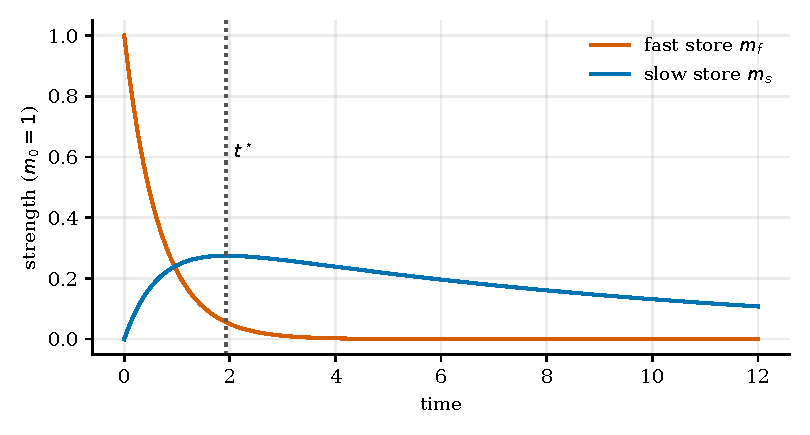
\includegraphics[width=0.85\textwidth]{figs/two_store}
\caption{Closed-form solution of Proposition~\ref{prop:twostore} for $\gamma=1$, $\kappa=0.5$, $\delta=0.1$. The slow store peaks at $t^\star$ and then decays at the slow rate. Computed by the script \texttt{figs.py} with seed 8; an illustration of the stated analytic result and not an evaluation of the architecture.}\label{fig:twostore}
\end{figure}

\section*{Worked consolidation: the two-store peak and a three-store cascade}\label{sec:cascade27}

The closed form of Proposition~\ref{prop:twostore} supports several quantities that can be computed exactly, and a cascade of more than two stores can be handled by the same method. This section gives the numbers for the parameters of Figure~\ref{fig:twostore}, treats the degenerate case that the proposition excludes, and states the cascade as a proposed extension whose proof is a partial-fraction computation.

\begin{workedex}[Peak time and transfer efficiency]\label{ex:twostore27}
Take $\gamma=1$, $\kappa=\tfrac12$ and $\delta=\tfrac1{10}$, so that $a=\tfrac32$. The slow store peaks at $t^\star=\ln(15)/1.4=\ntstar$, at which time the fast store retains $m_f(t^\star)=\nmftstar\,m_0$ and the slow store holds its maximum $m_s(t^\star)=\nmspeak\,m_0$. The maximum has the closed form
\begin{equation}
m_s(t^\star)=\frac{\kappa m_0}{a}\Bigl(\frac{\delta}{a}\Bigr)^{\delta/(a-\delta)},
\end{equation}
which follows by substituting $e^{-at^\star}=(\delta/a)\,e^{-\delta t^\star}$ and $e^{-\delta t^\star}=(\delta/a)^{\delta/(a-\delta)}$ into the solution, and it agrees with the numerical maximum to four decimals. The factor $\kappa/a=\ntransfer$ is the fraction of the initial strength that is ever transferred to the slow store, since the fast store loses strength at the total rate $a$ and the share $\kappa/a$ of that flow goes to replay; the peak is below this ceiling because the slow store is already decaying during the transfer. The consequence for design is that replay efficiency, $\kappa/(\gamma+\kappa)$, caps the slow-store strength before the slow decay rate $\delta$ is considered, so raising $\kappa$ and lowering $\gamma$ are not interchangeable with lowering $\delta$.

The case $a=\delta$ is excluded from Proposition~\ref{prop:twostore} because the denominator vanishes. Taking the limit of the solution gives $m_s(t)=\kappa m_0\,te^{-at}$, with maximum $\kappa m_0/(ae)$ at $t=1/a$. For $\gamma=\kappa=\tfrac12$ and $\delta=1$ this is $\ndegpeak\,m_0$ at $t=\ndegpeakt$, which the matrix exponential reproduces.
\end{workedex}

\begin{extension}[Cascade of $n$ stores]\label{ext:cascade27}
Let store $i$ lose strength at rate $a_i$ and pass strength to store $i+1$ at rate $k_i\le a_i$, with $m_1(0)=m_0$ and $m_i(0)=0$ for $i>1$, and let the rates $a_1,\dots,a_n$ be distinct. Then
\begin{equation}
m_n(t)=m_0\Bigl(\prod_{i=1}^{n-1}k_i\Bigr)\sum_{i=1}^n\frac{e^{-a_it}}{\prod_{j\ne i}(a_j-a_i)},
\end{equation}
and the total strength ever delivered to store $n$ is $m_0\prod_{i=1}^{n-1}k_i/a_i$.
\end{extension}

\begin{proof}
The Laplace transform of the cascade gives $\hat m_n(s)=m_0\prod_{i<n}k_i\big/\prod_{i\le n}(s+a_i)$. Since the roots $-a_i$ are simple, partial fractions give residues $1/\prod_{j\ne i}(a_j-a_i)$ at $s=-a_i$, and inversion gives the sum. For the delivered strength, store $i$ passes on the fraction $k_i/a_i$ of what it loses, and the product of these fractions along the chain is the share that reaches store $n$.
\end{proof}

The formula is the Bateman solution for a decay chain, a classical result, and it is used here for the memory interpretation and not as a new theorem.

\begin{workedex}[Three-store cascade]\label{ex:cascade27}
Take exit rates $(a_1,a_2,a_3)=(1.5,0.4,0.1)$ and transfer rates $(k_1,k_2)=(0.5,0.3)$. The second store peaks at $t=\ln(a_1/a_2)/(a_1-a_2)=\nmBpeakt$, and the third at $t=\nmDpeakt$ with strength $\nmDpeak\,m_0$, so the deeper store peaks later and lower, as the sequence of timescales requires. The strength ever delivered to the third store is $k_1k_2/(a_1a_2)=\ndelivthree\,m_0$, and the numerical integral of $a_3m_3$ over the whole time axis reproduces it, which is the conservation statement in the extension. The cascade quantifies the cost of depth: each added store multiplies the available strength by the transfer fraction $k_i/a_i$ and delays the peak, so a deep hierarchy is justified only when the recollections it serves are those that the shallow stores lose first.
\end{workedex}


\chapter{Reconsolidation and Memory Modification}\label{ch:reconsol}

The retrieval of a trace can render it labile and subject to modification before it is stabilized again, a process observed in experimental work on reconsolidation after retrieval \cite{nader2000}. In Mem8 the corresponding operation is a controlled post-retrieval update,
\begin{equation}\label{eq:reconsol}
M_{t+1}=M_t+\eta\,\mathcal U(M_t,r_t,c_t,Z_t),
\end{equation}
where $\mathcal U$ is an update direction computed from the retrieved reconstruction, the cue, and the context. Two requirements separate admissible updating from uncontrolled rewriting. The first is that the update be supported by evidence: $\mathcal U$ must depend on information that is external to the memory's own output, such as a new observation that conflicts with the retrieved reconstruction, and its magnitude must be gated by a statistic that measures the strength of that evidence. The second is that the record of what was previously stored be preserved, so that every revision can be audited and reversed.

The danger of an update that does not depend on external evidence can be stated exactly. Suppose that retrieval pulls each stored trace toward the reconstruction it helped produce, $\mathcal U_i=w_i(r-m_i)$, which is the natural form of an update driven by the memory's own output.

\begin{proposition}[Self-reinforcing distortion]\label{prop:drift}
If the update $m_i^+=m_i+\eta w_i(r-m_i)$ is applied with the reconstruction $r$ and the weights $w_i$ held fixed, then $m_i^+-r=(1-\eta w_i)(m_i-r)$. After $n$ repetitions the deviation of trace $i$ from $r$ is $(1-\eta w_i)^n(m_i-r)$, which tends to zero for every trace with $w_i>0$.
\end{proposition}

\begin{proof}
Subtract $r$ from both sides of the update. Iterating gives the stated power.
\end{proof}

Repeated retrieval under such a rule therefore collapses the traces that participate in a reconstruction onto that reconstruction, erasing the distinctions among them: what is remembered becomes what was last reconstructed, which is a formalization of the drift toward schema-consistent reproduction observed in serial reproduction studies \cite{bartlett1932}. The fixed-weights assumption makes the statement exact, and the qualitative conclusion, that distinctness is lost through self-generated updates, does not depend on it. Evidence-supported updating replaces $r$ in the update by an evidence-bearing target $e$ and gates the update by a likelihood-ratio statistic $\Lambda(e,r)$, the ratio of the probability of the evidence under the hypothesis that the retrieved reconstruction is outdated to its probability under the hypothesis that it is correct: $\mathcal U_i=g(\Lambda)\,w_i(e-m_i)$ with $g(\Lambda)=0$ below a threshold and increasing above it. A policy of this form changes a trace only when the world has told the system that it should.

The second requirement is satisfied by logging. If every update is recorded with the exact vector $\eta\,\mathcal U_s$ that was applied, then any earlier state is recoverable from a later one.

\begin{proposition}[Reversibility of logged updates]\label{prop:reverse}
If updates follow \eqref{eq:reconsol} and the ledger stores each increment $\Delta_s=\eta\,\mathcal U(M_s,r_s,c_s,Z_s)$ exactly, then $M_t=M_T-\sum_{s=t}^{T-1}\Delta_s$ for every $t\le T$.
\end{proposition}

\begin{proof}
Telescoping the recursion $M_{s+1}=M_s+\Delta_s$ from $s=t$ to $T-1$.
\end{proof}

The proposition is elementary and its consequence is the design rule of Chapter~\ref{ch:provenance}: memory modification must not silently rewrite the record of what was previously stored, and a log of increments, together with the evidence that triggered each, makes the history of a memory a first-class and recoverable object.

Figure~\ref{fig:drift} simulates the update of Proposition~\ref{prop:drift} with weights and reconstruction recomputed at every step. Traces that participate in the reconstruction collapse toward one another, while the gated update, which changes nothing without external evidence, leaves their separation intact.

\begin{figure}[t]
\centering
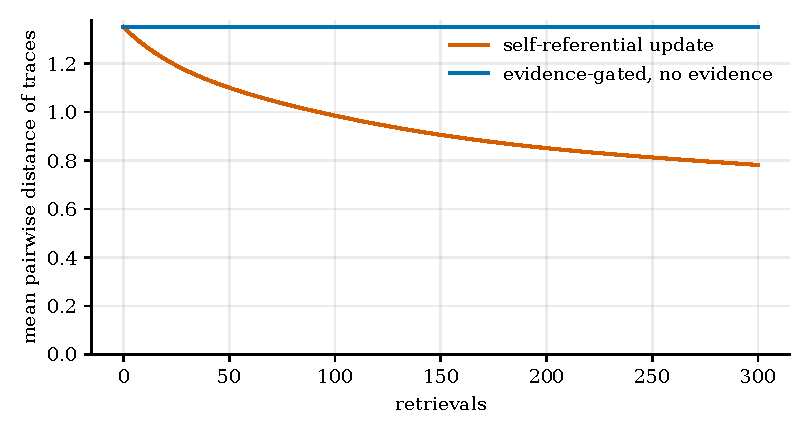
\includegraphics[width=0.85\textwidth]{figs/drift}
\caption{Mean pairwise distance among five stored traces under repeated retrieval with a self-referential update ($\eta=0.05$, $\beta=6$, fixed cue), compared with an evidence-gated update that receives no evidence. Computed by the script \texttt{figs.py} with seed 8; an illustration of the stated analytic result and not an evaluation of the architecture.}\label{fig:drift}
\end{figure}

\section*{Drift and gating: numbers and a counterexample}\label{sec:gate28}

Proposition~\ref{prop:drift} states the collapse qualitatively, and the evidence gate of the preceding discussion is a design rule whose content depends on how its statistic is computed. Two short examples fix the scale of the first and show a way in which the second can fail.

\begin{workedex}[Scale of self-reinforcing drift]\label{ex:drift28}
Hold the weight on a participating trace at $w_i=0.4$ and take the update rate $\eta=0.05$, so the contraction factor per retrieval is $1-\eta w_i=0.98$. After $n=50$ retrievals the trace retains the fraction $0.98^{50}=\ndriftfac$ of its original deviation from the reconstruction, and the deviation halves after $\nhalflifedrift$ retrievals. The collapse is therefore not a fast phenomenon at these rates: a trace that is retrieved fifty times has lost nearly two thirds of its distinctness from its neighbours, and the policy matters in the regime of heavily rehearsed material, which is the regime in which memory is least often checked against the world.
\end{workedex}

\begin{counterex}[Correlated reports pass the gate]\label{cex:gate28}
Suppose the gate opens when the likelihood ratio statistic $\Lambda$ reaches $\Lambda^\ast=10$, and that $\Lambda$ is computed as the product of the likelihood ratios of the individual reports, which is correct when the reports are conditionally independent given the hypothesis. A single report from a source that is correct with probability $0.7$ has likelihood ratio $\ell=0.7/0.3=\nellrep$. Three conditionally independent reports give $\Lambda=\ell^3=\nlamnaive>\Lambda^\ast$ and the gate opens. If the three reports are three copies of one observation, as when one source is relayed three times, the same product still gives $\nlamnaive$, whereas the correct likelihood ratio of the single underlying observation is $\nlamcopy<\Lambda^\ast$ and the gate should stay closed. The statistic is inflated by the factor $\ell^{k-1}$ for $k$ copies, which is $\ell^2=5.44$ here.
\end{counterex}

The counterexample is about the computation of the gate and not about the gate. The minimum number of conditionally independent reports of ratio $\ell$ needed to open a gate with threshold $\Lambda^\ast$ is $\lceil\ln\Lambda^\ast/\ln\ell\rceil$, which equals three for the values above because $\ln10/\ln(7/3)=\nnclusters$, and the count is meaningful only if the reports are independent. The ledger of Chapter~\ref{ch:provenance} supplies the required discipline, since every evidence record carries its source, so the gate can aggregate by source and count each at most once. This is a design constraint on the architecture and it is not a theorem about the world: sources can be correlated without being identical, and the treatment of partial dependence is left to the protocols of Part~IX.


\chapter{Forgetting, Interference, and Resource Constraints}\label{ch:forgetting}

Forgetting is defined in three ways, and the three are not equivalent. It may be a decline of recoverability, so that Definition~\ref{def:recov} fails for cue families that formerly satisfied it. It may be an increase of reconstruction cost, so that the trace remains recoverable only through a longer iteration or a more specific cue. It may be a deliberate release of a representational commitment, in which the system removes content, leaving in the ledger a record that the removal occurred. A theory that recognized only the first would treat all forgetting as loss, whereas the second and third are often the efficient and the required behavior.

The retrieval score gives amplitude decay a specific and sometimes unexpected consequence. If a stored trace of unit direction decays in amplitude as $m(t)=e^{-\gamma t}\hat m$ and the query is the aligned unit vector, then $\rho=2e^{-\gamma t}/(1+e^{-2\gamma t})=\operatorname{sech}(\gamma t)$ and by Theorem~\ref{thm:closed}
\begin{equation}\label{eq:decayscore}
S\bigl(m(t),\hat m\bigr)=\frac{\operatorname{sech}(\gamma t)}{2}\bigl(1+\operatorname{sech}(\gamma t)\bigr),
\end{equation}
which falls monotonically from one at $t=0$ toward zero, whereas the cosine of the same pair does not change with amplitude at all. Under the resonance score an older, weaker trace is therefore penalized relative to a newer one of equal alignment, producing a recency preference as a direct consequence of the energy-balance factor and without any dedicated mechanism. Whether this preference is desirable is a matter of policy: it is appropriate when recency predicts relevance and inappropriate when the old trace is the better evidence. The corollary for architecture is that amplitude must be treated as a managed quantity, either normalized at write time and given an explicit age feature, or allowed to carry age deliberately, and that the choice must be recorded as part of the specification.

Resource-sensitive forgetting is the policy of choosing which traces to release when a budget is binding. The comparison with indiscriminate temporal decay is clean in the simplest case.

\begin{proposition}[Optimal retention under a budget]\label{prop:retention}
Suppose each of $N$ items will be queried in the future independently with probabilities $p_1,\dots,p_N$, a query for a retained item succeeds and a query for a released item fails, and at most $B$ items can be retained. The retention set that maximizes the expected number of successful queries is the set of $B$ items with the largest $p_i$. A policy that retains the $B$ youngest items attains the optimum if and only if the access probability is nonincreasing in age, in the sense that the youngest $B$ items are among the $B$ largest $p_i$.
\end{proposition}

\begin{proof}
The expected number of successes is $\sum_{i\in R}p_i$ over the retained set $R$, which is maximized under the cardinality constraint by selecting the $B$ largest values. The age-based policy selects the $B$ youngest, which coincides with this set exactly when those items carry the $B$ largest probabilities.
\end{proof}

The proposition does not say that decay is wrong; it says that decay is optimal precisely when age is a sufficient statistic for future access, and that where other predictors are available, such as the number of distinct contexts in which an item was previously retrieved, the provenance of the item, or its dependence by other retained items, a better policy exists. The monograph compares learned and rule-based retention policies against age-based decay in Chapter~\ref{ch:scaling} at matched budgets, and deliberate release is implemented by tombstone records that remove the content while preserving in the ledger the facts that the trace existed and that it was released, with the content removed in full when erasure is required.

\section*{Retention and recency: a counterexample and a closed form}\label{sec:retain29}

\begin{counterex}[Youngest-first retention is not optimal]\label{cex:retain29}
Let six items, listed from youngest to oldest, have future access probabilities $(0.10,0.50,0.05,0.30,0.02,0.40)$ and let the budget be $B=3$. The age-based policy retains the three youngest and obtains an expected $\nretyoung$ successful queries, while the optimal policy of Proposition~\ref{prop:retention} retains the items with probabilities $0.50$, $0.40$ and $0.30$ and obtains $\nretopt$. The regret is $\nregret$ expected queries, nearly half of the optimum. The example is built so that age is a poor predictor, and the proposition says exactly when this happens: the age policy is optimal if and only if the youngest $B$ items are the $B$ most probable. Whether any real memory has access probabilities of this form is a matter of measurement, and the example makes no claim about it.
\end{counterex}

\begin{workedex}[Recency from the energy-balance factor]\label{ex:recency29}
For a trace decaying as $m(t)=e^{-\gamma t}\hat m$ and an aligned unit query, equation~\eqref{eq:decayscore} gives scores that depend only on $\gamma t$. At $\gamma t=1$ one has $\operatorname{sech}(1)=\nrhoB$ and $S=\nSdecayB$, at $\gamma t=2$ one has $\nrhotwo$ and $\nSdectwo$, and at $\gamma t=3$ one has $\nrhothree$ and $\nSdecthree$, while the cosine of the same pair stays at one throughout. The score falls to one half when $\rho(1+\rho)=1$, that is, when $\rho$ is the reciprocal of the golden ratio, and the corresponding age is $\gamma t=\operatorname{arcosh}\varphi=\ngtheigh$. The resonance score therefore imposes a definite recency scale on a store in which amplitude decays, and the scale is set by $\gamma$ alone: a trace loses half its score at about one decay time, regardless of its alignment. This is a consequence of the closed form of Theorem~\ref{thm:closed} and not a finding about memory.
\end{workedex}


\chapter{Memory Compression and Future Admissibility}\label{ch:compression}

Compression of a store is acceptable not when it reduces storage by some factor but when it preserves what future reconstruction needs. Let $\mathcal Q$ be a family of admissible future queries, let $C$ be a compression map applied to the memory state, and let $d$ be a distance on reconstructions. The objective is a bound
\begin{equation}\label{eq:compbound}
\sup_{q\in\mathcal Q}d\bigl(\Eph(q,M),\Eph(q,C(M))\bigr)\le\varepsilon,
\end{equation}
which ties the permitted loss directly to preserved reconstructive capacity and not to a storage criterion. Two limiting cases clarify the content of the bound. If $C$ factors through the quotient by recollective equivalence, in the sense that $C(M)$ determines the class of $M$ under $\sim_{\mathcal Q}$, then the supremum is zero for any $\varepsilon\ge0$, and the compression is lossless with respect to $\mathcal Q$; this is the sufficiency theorem of Chapter~\ref{ch:ident} in the language of compression. At the other extreme, a compression that discards any distinction that some query in $\mathcal Q$ depends on has a strictly positive supremum, whatever its storage savings.

For the softmax reconstruction the bound can be made explicit.

\begin{proposition}[Distortion bound for the softmax readout]\label{prop:distort}
Let $M=(m_1,\dots,m_P)$ and $M'=(m_1',\dots,m_P')$ be stores with $\norm{m_i},\norm{m_i'}\le1$ and $\max_i\norm{m_i-m_i'}\le\delta$, and let $F_M(c)=\sum_iw_i(c)m_i$ with $w=\softmax(\beta\ip{m_i}{c})$ for a query $c$ with $\norm c\le1$. Then $\norm{F_M(c)-F_{M'}(c)}\le(1+2\beta)\delta$.
\end{proposition}

\begin{proof}
The scores differ by at most $\delta$ in each coordinate, since $|\ip{m_i-m_i'}{c}|\le\delta$. The derivative of the softmax is $\beta(\operatorname{diag}(w)-ww^\top)$, and for a perturbation $v$ with $\norm v_\infty\le\delta$ its image has $\ell_1$ norm at most $\beta\sum_iw_i|v_i-\bar v|\le2\beta\delta$, with $\bar v=\sum_jw_jv_j$. Integrating along the segment between the two score vectors gives $\norm{w-w'}_1\le2\beta\delta$. Then $\norm{F_M-F_{M'}}\le\norm{\sum_i(w_i-w_i')m_i}+\norm{\sum_iw_i'(m_i-m_i')}\le2\beta\delta+\delta$.
\end{proof}

The bound shows that the distortion permitted to each trace is inversely proportional to $1+2\beta$, so sharper selection, which is useful for discrimination, makes the readout more sensitive to compression error, and therefore trades against compressibility. For the storage cost of achieving a given per-trace distortion, the rate--distortion function of a Gaussian source with independent components of variance $\sigma^2$ under squared error is $R(D)=\frac12\log_2(\sigma^2/D)$ bits per component for $D<\sigma^2$ \cite{cover2006}. For a trace with $d$ real components and a target distortion $\norm{m-m'}^2\le\delta^2$, with $D=\delta^2/d$ per component, this gives
\begin{equation}
R(\delta)=\frac d2\log_2\frac{d\sigma^2}{\delta^2}\ \text{bits per trace},\qquad\delta^2<d\sigma^2,
\end{equation}
as a lower bound on the representation size under this source model, and the budget of Proposition~\ref{prop:distort} then fixes $\delta$ from the desired reconstruction accuracy. For low-rank compression of a store matrix, the Eckart--Young theorem states that the best rank-$k$ approximation in the Frobenius norm has error $\bigl(\sum_{j>k}\sigma_j^2\bigr)^{1/2}$ in terms of the singular values of the store, and each trace is perturbed by at most that amount, so the singular spectrum of the store determines how far it can be compressed under a given $\varepsilon$ \cite{eckart1936}. These are bounds under stated source models, and the monograph treats the sufficiency-based compression, which discards by equivalence class and not by magnitude, as the quantity of primary interest, since it can compress by much more than any magnitude-based method when most of the stored structure is irrelevant to the admissible queries.

\section*{How tight is the distortion bound?}\label{sec:distort30}

Proposition~\ref{prop:distort} bounds the change of the softmax readout under a perturbation of the store by $(1+2\beta)\delta$. Two questions about this bound can be answered by computation: how loose it is on typical stores, and whether its linear growth in $\beta$ is an artifact of the proof.

\begin{workedex}[Looseness on random stores]\label{ex:looseness30}
In 300 random stores with $3\le P\le19$ traces in dimensions $4$ to $29$, inverse temperatures drawn uniformly from $[0.5,15]$, perturbations of size up to $0.1$, and five random cues each, the largest observed ratio of $\norm{F_M(c)-F_{M'}(c)}$ to $(1+2\beta)\delta$ was $\ncompratio$. The bound therefore held in every instance and was typically loose by a factor of several, as expected of a worst-case bound on random data. This is an algebraic check of the proposition, with a fixed seed, and it is not a statement about any memory system.
\end{workedex}

\begin{extension}[The linear dependence on $\beta$ is necessary]\label{ext:sharp30}
There are stores and queries for which $\norm{F_M(c)-F_{M'}(c)}\ge\tfrac{\sqrt3}{2}\tanh(\beta\delta/2)$ with $\max_i\norm{m_i-m_i'}=\delta$. Consequently $\sup\norm{F_M-F_{M'}}/\delta\ge\tfrac{\sqrt3}{4}\beta(1+o(1))$ as $\delta\to0$ for each fixed $\beta$, and the factor $1+2\beta$ in Proposition~\ref{prop:distort} cannot be replaced by any function that is $o(\beta)$.
\end{extension}

\begin{proof}
In $\R^2$ take the cue $c=(1,0)$ and the traces $m_1=(\tfrac12,\tfrac{\sqrt3}2)$ and $m_2=(\tfrac12,-\tfrac{\sqrt3}2)$, which are unit vectors with equal scores $\tfrac12$ against $c$. Perturb $m_1$ to $m_1'=m_1+\delta c$. Then $w_1'=1/(1+e^{-\beta\delta})$ and $w_2'=1-w_1'$, and $F_{M'}-F_M$ has second coordinate $\tfrac{\sqrt3}2(w_1'-w_2')=\tfrac{\sqrt3}2\tanh(\beta\delta/2)$, since the unperturbed weights are equal and the second coordinates of $m_1$ and $m_2$ are opposite. The norm is at least the absolute value of this coordinate, and $\tanh(x)\ge x(1+o(1))$ as $x\to0$.
\end{proof}

For $\beta=10$ and $\delta=0.01$ the exact ratio $\norm{F_M-F_{M'}}/\delta$ is $\nsharpvalBA$ against the proposition's bound of $21$, and for $\beta=40$ and $\delta=0.0025$ it is $\nsharpvalEA$ against $81$. The ratios to the bound are $\nsharpBA$ and $\nsharpEA$, so the bound is tight up to a factor of about five in this family and the proof's linear dependence on $\beta$ reflects a real sensitivity. A store sharp enough for selective recall in the sense of Chapter~\ref{ch:stability} is therefore a store whose readout is correspondingly sensitive to quantization or pruning of the traces, and the compression budget $\varepsilon$ of \eqref{eq:compbound} must be spent at a rate that scales inversely with $\beta$.

\section*{Synthesis of Part~VI}\label{sec:synth6}

The examples of this part share a structure: each chapter fixes a rate or a sensitivity, and the examples show that the rate is controlled by a small number of quantities that can be read off the model. In consolidation the controlling quantities are the exit rates and transfer fractions, which determine both when the deeper store peaks and how much strength it ever receives (Extension~\ref{ext:cascade27}), so that the delivered fraction $k_1k_2/(a_1a_2)=\ndelivthree$ is fixed by the rates before any content is considered. In reconsolidation the controlling quantity is the contraction factor $1-\eta w_i$ of the self-referential update, which sets the half-life of distinctness at $\nhalflifedrift$ retrievals for the example rates, together with the independence of the evidence that opens the gate (Counterexample~\ref{cex:gate28}). In forgetting it is the match between the retention rule and the access probabilities (Counterexample~\ref{cex:retain29}) and the recency scale $\operatorname{arcosh}\varphi$ that the energy-balance factor builds in (Worked Example~\ref{ex:recency29}). In compression it is the product of the inverse temperature and the perturbation size (Extension~\ref{ext:sharp30}).

The results connect through the temperature and through the sufficiency criterion. A store that is sharp enough for selective retrieval, with $\beta$ above the thresholds of Chapter~\ref{ch:stability}, is also a store that amplifies perturbations linearly in $\beta$, so the compression that consolidation performs when it moves strength into a slower, more overlapping store has a cost that grows with the selectivity it is meant to support. Reconsolidation determines whether the distinctions the slow store receives are distinctions of the world or of the system's own earlier reconstructions, and the gate computation determines whether the evidence for a revision is counted once or several times. Forgetting then decides, under a budget, which of the surviving traces are kept, and Proposition~\ref{prop:retention} is the statement that this decision should be made on predicted access and not on age unless age is a sufficient statistic. All four operations are changes to the stored state, and the criterion of Theorem~\ref{thm:suff} applies after each of them: an operation is admissible with respect to the committed recollections only if it does not merge histories that those recollections distinguish. Part~VII makes this the organizing principle, and the viability-preserving equivalence of Extension~\ref{ext:viabequiv} is the form that principle takes when the operations are repeated.

The same caveats hold as for Part~VII. The rates are those of linear models chosen so that the solutions are in closed form, the retention probabilities and the report likelihoods are constructed to expose a logical point, and none of these numbers is an estimate of a quantity in a biological or deployed memory. The numerical statements were produced by the script \texttt{examples.py} and cross-checked against the matrix exponential or by direct simulation as noted at each example.

\part{Formal Theory of Reconstructive Memory}

\chapter{State Spaces and Transition Systems}\label{ch:transition}

The formal theory begins by fixing what is a state, what is a transition, and what an observer can see. The system state is the tuple $X_t=(M_t,\Psi_t,\Theta_t,Z_t,H_t,B_t)$ of equation~\eqref{eq:state}, taking values in a measurable space $\mathcal X$, and the stochastic variant of the dynamics is the controlled Markov kernel
\begin{equation}\label{eq:kernel}
X_{t+1}\sim P_\vartheta(\,\cdot\mid X_t,c_t,a_t),
\end{equation}
where $c_t\in\Cues\cup\{\varnothing\}$ is the cue presented at step $t$ (or none), $a_t$ is an action drawn from a finite or compact action set that includes encoding an observation, changing the context, and allocating resources, and $\vartheta$ collects the parameters. Three maps complete the specification. The storage map $\Sigma:\mathcal X\times\mathcal O\to\mathcal X$ incorporates an observation $o$ into the persistent component, the observation function $\mathrm{obs}:\mathcal X\to\mathcal W$ reports whatever an external observer is permitted to read directly, and the ecphoric operator $\Eph:\Mem\times\Cues\times\mathcal Z\to\Recs$ produces a reconstruction. The deterministic variant is obtained when $P_\vartheta(\cdot\mid x,c,a)$ is a point mass $\delta_{f_\vartheta(x,c,a)}$, and the finite-dimensional approximation replaces $\mathcal X$ by a finite-dimensional manifold or by a finite set with the cardinalities fixed by the representation sizes of Chapter~\ref{ch:substrate}.

The distinction between the physical state and the accessible mnemonic state is the one that organizes the remaining chapters of the theory. The physical state is $X_t$ in full. The accessible state is its class under recollective equivalence, in the sense of Definition~\ref{def:equiv}: two physical states are mnemonically equivalent if no cue in the admissible family can separate them. For this reading to be coherent the equivalence classes must evolve consistently, so that two equivalent states are still equivalent after the same cue and action. When that holds the accessible state is itself a Markov system, and when it fails the accessible state is not a function of the accessible state at the previous step, so any prediction of recollection from the accessible state alone is incomplete. The condition is exactly the lumpability condition of Chapter~\ref{ch:projection}, and its failure is not a pathology: a memory in which two behaviorally equivalent states respond differently to a future encoding is a memory with hidden state.

\begin{proposition}[Accessible state is a Markov system exactly under lumpability]\label{prop:accmarkov}
Let $\pi:\mathcal X\to\mathcal A$ be the quotient map to accessible states under an equivalence $\sim$ on a finite state space, and let $P$ be a transition kernel for fixed $(c,a)$. The process $\pi(X_t)$ is a Markov chain with transition kernel $\bar P(\alpha,\alpha')=\sum_{x'\in\alpha'}P(x,x')$ for every initial distribution if and only if the sum on the right depends on $x$ only through $\pi(x)$.
\end{proposition}

\begin{proof}
This is the strong lumpability criterion of Kemeny and Snell \cite{kemeny1960}. Sufficiency: if the block-sum is a function of $\pi(x)$, the conditional law of $\pi(X_{t+1})$ given $X_0,\dots,X_t$ depends only on $\pi(X_t)$ and equals $\bar P$. Necessity: if two states $x,y$ in the same block have different block-sums into some block $\alpha'$, an initial distribution concentrated on $x$ and one concentrated on $y$ give the same $\pi(X_0)$ and different laws of $\pi(X_1)$, so $\bar P$ cannot be defined.
\end{proof}

\chapter{Observability and Reconstructive Identifiability}\label{ch:ident}

This chapter contains the central result of the monograph. It is deliberately elementary, in the sense that its proof is a few lines, because its force is in what it makes precise: the difference between a memory that preserves every distinction among histories and a memory that preserves exactly those distinctions that a specified family of future recollections needs.

Let $\Hist$ be a set of histories, $\Mem$ a set of persistent memory states, $\Cues$ a set of admissible cues, and $\Recs$ a set of reconstructions. An encoding is a map $E:\Hist\to\Mem$. A target recollection function $T:\Hist\times\Cues\to\Recs$ specifies what should be reconstructed from the history $h$ when the cue $c$ arrives. An ecphoric decoder is a map $D:E(\Hist)\times\Cues\to\Recs$, and its defining feature, which the theorem makes essential, is that it sees the memory state and the cue and nothing else. In particular it does not see the history.

\begin{definition}[Ecphoric sufficiency]\label{def:suff}
The encoding $E$ is \emph{sufficient} for $T$ on $\Cues$ if $E(h_1)=E(h_2)$ implies $T(h_1,c)=T(h_2,c)$ for all $c\in\Cues$. It is \emph{realized} by a decoder $D$ if $D(E(h),c)=T(h,c)$ for all $h\in\Hist$ and $c\in\Cues$.
\end{definition}

\begin{theorem}[Ecphoric sufficiency criterion]\label{thm:suff}
An encoding $E$ is realized by some decoder if and only if it is sufficient for $T$ on $\Cues$. When it is realized, the decoder is unique on $E(\Hist)\times\Cues$.
\end{theorem}

\begin{proof}
Suppose $D$ realizes $E$ and $E(h_1)=E(h_2)=m$. Then $T(h_1,c)=D(m,c)=T(h_2,c)$ for every $c$, so $E$ is sufficient. Conversely, suppose $E$ is sufficient. For $(m,c)$ with $m\in E(\Hist)$ choose any $h$ with $E(h)=m$ and set $D(m,c)=T(h,c)$. By sufficiency the value does not depend on the choice of $h$, so $D$ is well defined, and $D(E(h),c)=T(h,c)$ by construction. Uniqueness on $E(\Hist)\times\Cues$ holds because any decoder realizing $E$ must take the value $T(h,c)$ at $(E(h),c)$.
\end{proof}

The theorem makes no use of structure on $\Mem$, $\Cues$ or $\Recs$, and this is a feature. The oscillatory, resonant, attractor and inferential mechanisms of Parts~II to V are each a candidate way of computing $D$ within resource limits, and the theorem says that none of them can succeed where the criterion fails. The criterion itself is a purely informational statement about $E$ and $T$. Its content becomes visible in the minimal sufficient memory.

\begin{definition}[Recollective profile and equivalence of histories]\label{def:profile}
The profile of a history is the function $\tau_h=T(h,\cdot):\Cues\to\Recs$. Two histories are recollectively equivalent, $h_1\approx_Th_2$, if $\tau_{h_1}=\tau_{h_2}$.
\end{definition}

\begin{corollary}[Minimal sufficient memory]\label{cor:minimal}
The encoding $E$ is sufficient for $T$ on $\Cues$ if and only if there is a map $\phi:E(\Hist)\to\Hist/\!\approx_T$ with $\phi\circ E=[\cdot]_T$, where $[\cdot]_T$ is the quotient map. Equivalently, $\approx_T$ is a coarsening of the kernel equivalence of $E$. In particular the quotient encoding $[\cdot]_T$ is sufficient and every sufficient encoding factors through it in the sense that it determines it; the cardinality $|\Hist/\!\approx_T|$ is the smallest number of distinct memory states a sufficient encoding can use.
\end{corollary}

\begin{proof}
Sufficiency says that the kernel equivalence of $E$ refines $\approx_T$, which is precisely the existence of $\phi$ with $\phi\circ E=[\cdot]_T$ (a map defined on the image of $E$ by $\phi(E(h))=[h]_T$, well defined by refinement). For the cardinality, $\phi$ is onto $\Hist/\!\approx_T$ because every class contains some $h$, hence $|E(\Hist)|\ge|\Hist/\!\approx_T|$.
\end{proof}


\begin{figure}[t]
\centering
\begin{tikzpicture}[>=Stealth,node distance=3.2cm,every node/.style={font=\small}]
\node (H) {$\Hist$};
\node (M) [right=of H] {$E(\Hist)\subseteq\Mem$};
\node (Q) [below=2.2cm of M] {$\Hist/{\approx_T}$};
\node (Y) [right=3.6cm of M] {$\Recs^{\Cues}$};
\draw[->] (H) -- node[above] {$E$} (M);
\draw[->] (H) -- node[below left] {$[\cdot]_T$} (Q);
\draw[->,dashed] (M) -- node[right] {$\phi$} (Q);
\draw[->] (M) -- node[above] {$D(\cdot,c)_{c\in\Cues}$} (Y);
\draw[->] (Q) -- node[below right] {$\tau$ (injective)} (Y);
\end{tikzpicture}
\caption{Sufficiency as factorization (Theorem~\ref{thm:suff} and Corollary~\ref{cor:minimal}). The profile map $\tau$ sends a class of histories to its recollective profile; $E$ is sufficient exactly when the dashed map $\phi$ exists, and the decoder is then $D=\tau\circ\phi$.}\label{fig:factor}
\end{figure}

The corollary is the formal content of the phrase that memory preserves conditions for reinstatement and not the history itself. Two histories that differ in ways that no admissible cue can reveal through $T$ need not be distinguished by the memory, and any storage that does distinguish them is surplus with respect to $T$. The same distinctions may of course matter for a different target $T'$, which is why the target must be fixed as part of the specification and not left implicit. The example of Chapter~\ref{ch:intro} shows the failure in its smallest form: for $E(a,b)=e_a+e_b$ one has $E(a,b)=E(b,a)$, and a target that returns the first item of the pair has $T((a,b),c)\ne T((b,a),c)$ for every cue that does not reveal order, so no decoder exists however the retrieval dynamics are designed.

The exact criterion is brittle in one respect, since real decoders return approximations. The approximate version is stated for a metric $d$ on $\Recs$.

\begin{theorem}[Approximate sufficiency]\label{thm:approx}
Let $(\Recs,d)$ be a metric space and $\varepsilon\ge0$. For $m\in E(\Hist)$ and $c\in\Cues$ write $A(m,c)=\{T(h,c):E(h)=m\}$. A decoder with $d\bigl(D(E(h),c),T(h,c)\bigr)\le\varepsilon$ for all $h,c$ exists if and only if every set $A(m,c)$ is contained in a closed ball of radius $\varepsilon$. A necessary condition is $\operatorname{diam}A(m,c)\le2\varepsilon$ for all $(m,c)$, and if every set of diameter $\delta$ in $\Recs$ lies in a ball of radius $\delta/2$, which holds on the real line and, more generally, in hyperconvex spaces such as $\ell_\infty^k$, the condition $\operatorname{diam}A(m,c)\le2\varepsilon$ is also sufficient.
\end{theorem}

\begin{proof}
Given such a decoder, the center $D(m,c)$ is within $\varepsilon$ of every element of $A(m,c)$, so the set lies in the ball $\bar B(D(m,c),\varepsilon)$. Conversely, choose for each $(m,c)$ a center $y_{m,c}$ of a closed ball of radius $\varepsilon$ containing $A(m,c)$ and set $D(m,c)=y_{m,c}$. Necessity of the diameter bound follows from the triangle inequality through the center, giving $d(y,y')\le2\varepsilon$ for $y,y'\in A(m,c)$. For the final statement, if $\operatorname{diam}A\le2\varepsilon$ and the set lies in a ball of radius $\operatorname{diam}A/2\le\varepsilon$, the first part applies.
\end{proof}

The factor of two between the necessary and the sufficient conditions is real in general metric spaces and is the price of not assuming that sets of a given diameter have centers close to their elements. In Euclidean space Jung's theorem reduces the gap from a factor of two to a factor of $\sqrt2$, a refinement that does not change the structure of the argument.

The next result quantifies what the absence of sufficiency costs. It concerns the recovery of the history itself, which is the extreme target $T(h,c)=h$.

\begin{proposition}[Identifiability limit]\label{prop:identlimit}
Let $\Hist$ be finite with prior $p$ and let $E$ be deterministic. The maximum over decoders $\hat h:E(\Hist)\to\Hist$ of the probability of recovering $h$ is
\begin{equation}
\max_{\hat h}\Pr[\hat h(E(h))=h]=\sum_{m\in E(\Hist)}\max_{h:E(h)=m}p(h),
\end{equation}
which equals $|E(\Hist)|/|\Hist|$ under the uniform prior. Moreover, for any estimator, Fano's inequality gives
\begin{equation}
\Pr[\hat h(E(h))\ne h]\ \ge\ \frac{H(h\mid E(h))-\log2}{\log|\Hist|}.
\end{equation}
\end{proposition}

\begin{proof}
Given $m$, the decoder must name one history in the fiber $E^{-1}(m)$, and the probability of being correct conditional on $m$ is maximized by the history of greatest prior mass; summing over fibers weighted by the probability of the fiber gives the first expression. Under the uniform prior each fiber has maximum mass $1/|\Hist|$ and there are $|E(\Hist)|$ fibers. Fano's inequality is the standard inequality \cite{cover2006} applied to the variable $h$ and its estimate through $E(h)$, and $H(h\mid E(h))=H(h)-H(E(h))$ for deterministic $E$.
\end{proof}

Two aspects of this bound deserve emphasis. It is independent of the retrieval mechanism, so no amount of recurrent refinement, phase coordination, or learned inference can raise the accuracy above $|E(\Hist)|/|\Hist|$ when only the memory state is consulted. And it concerns recovery of the whole history, so it is an upper bound on the ability to answer every possible question, not on the ability to answer the questions in $T$; Theorem~\ref{thm:suff} is the relevant criterion when the target is narrower. The two together define the extent to which statements about the fidelity of a memory system are statements about the encoding and not about the decoder. A general lesson is that observation of poor reconstruction does not by itself implicate the retrieval dynamics, and a diagnostic that separates the two is to hold the encoding fixed and ask whether Theorem~\ref{thm:suff} is satisfied for the target of interest.

Two qualifications limit how the theorem may be used. The first is that the decoder is assumed to have no additional information; if the decoder can consult the ledger of Chapter~\ref{ch:provenance} or any other store, then that store is part of the memory state and the criterion applies to the combined encoding. The second is that sufficiency is a property of the pair $(E,T)$ together with the cue family, so the claim that a system is sufficient is empty until the cue family is stated, and a system can be sufficient for one family and insufficient for a larger one; this is the formal reason that a design must record the family of future recollections it commits to supporting.

\section*{A finite history space: destroyed and preserved distinctions}\label{sec:finite32}

The criterion is easiest to appreciate on a history space small enough to enumerate. The material of this section is a worked example followed by a proposed extension to noisy encodings; the first is an exercise in Theorem~\ref{thm:suff}, and the second is proved here from elementary decision theory and is not drawn from the memory literature.

\begin{workedex}[Three encodings of a six-element history space]\label{ex:finite32}
Let a history record what was encountered and where, $\Hist=\{a,b,c\}\times\{0,1\}$, so that $h=(x,y)$ has $|\Hist|=6$, and let the prior be uniform. A single future cue asks where the item was seen, so $\Cues=\{c_{\mathrm{where}}\}$ and $T(h,c_{\mathrm{where}})=y$. Consider three encodings: $E_1(x,y)=x$, which keeps the identity of the item and discards the location; $E_2(x,y)=y$, which keeps the location and discards the identity; and $E_3(x,y)=(\bar x,y)$ with $\bar a=\bar b=\mathsf{ab}$ and $\bar c=\mathsf c$, which keeps the location and merges two of the three items. The kernel classes are
\begin{align}
\ker E_1&=\bigl\{\{(a,0),(a,1)\},\{(b,0),(b,1)\},\{(c,0),(c,1)\}\bigr\},\\
\ker E_2&=\bigl\{\{(a,0),(b,0),(c,0)\},\{(a,1),(b,1),(c,1)\}\bigr\},\\
\ker E_3&=\bigl\{\{(a,0),(b,0)\},\{(a,1),(b,1)\},\{(c,0)\},\{(c,1)\}\bigr\},
\end{align}
with $\nnstatesone$, $\nnstatestwo$ and $\nnstatesthree$ classes respectively. The recollective equivalence $\approx_T$ has exactly two classes, $\{y=0\}$ and $\{y=1\}$, since $\tau_h$ depends on $h$ only through $y$. By Corollary~\ref{cor:minimal} an encoding is sufficient exactly when its kernel is contained in $\approx_T$. The kernel of $E_1$ is not contained in $\approx_T$, because the class $\{(a,0),(a,1)\}$ joins two histories with different locations. The kernels of $E_2$ and $E_3$ are contained in $\approx_T$, so both are sufficient, and $E_2$ is the minimal one with $|\Hist/\!\approx_T|=2$ memory states.

For the sufficient encodings the decoder is the one constructed in the proof of Theorem~\ref{thm:suff}: choose a representative of each fiber and read off its location. For $E_2$ it is the table $D_2(0,c_{\mathrm{where}})=0$ and $D_2(1,c_{\mathrm{where}})=1$, and for $E_3$ it is $D_3((\mathsf{ab},y),c_{\mathrm{where}})=D_3((\mathsf c,y),c_{\mathrm{where}})=y$. The tables are explicit and the check $D(E(h),c_{\mathrm{where}})=T(h,c_{\mathrm{where}})$ passes on all six histories. For $E_1$ no table exists. The fiber $\{(a,0),(a,1)\}$ forces a single answer for two different targets, so any decoder errs on at least one of them, and under the uniform prior the best decoder answers correctly with probability one half.
\end{workedex}

The example also separates two quantities that are easily conflated. By Proposition~\ref{prop:identlimit} the accuracy of recovering the whole history is $|E(\Hist)|/|\Hist|$, which equals $\nidaccone$ for $E_1$, $\nidacctwo$ for $E_2$ and $\nidaccthree$ for $E_3$. The encoding that is worst for the stated target, $E_1$, is better than the best minimal encoding at recovering histories, and the ordering of the three encodings by identifiability is not the ordering by sufficiency. This is the quantitative form of the statement that fidelity to the history and sufficiency for a family of recollections are different properties.

\begin{counterex}[Sufficiency is relative to the cue family]\label{cex:cuefamily}
Enlarge the cue family by a second cue, $c_{\mathrm{what}}$, with $T(h,c_{\mathrm{what}})=x$. The recollective equivalence on $\Hist$ is now the identity, since $\tau_h$ determines both coordinates. Then $E_3$, which was sufficient for $c_{\mathrm{where}}$, fails: the class $\{(a,0),(b,0)\}$ joins histories with different answers to $c_{\mathrm{what}}$. The best decoder for the new cue under the uniform prior has error $\nriskthreewhat$, because in each of the two merged classes the decoder must guess between two equally likely items. The encoding $E_2$ fails for the same reason. Only the identity encoding is sufficient for both cues, and it needs all six states. The example shows that the claim ``the encoding is sufficient'' carries an implicit quantifier over the cue family, which is why the family must be recorded in the specification.
\end{counterex}

The three failures above were exact. A deployed memory is noisy, so the memory state is a random variable whose law depends on the history, and the right question is how small the error can be made when the criterion holds only up to a channel.

\begin{extension}[Bayes risk of noisy ecphory]\label{ext:bayesrisk}
Let $\Hist$ be finite with prior $\pi$, and let the encoding be a stochastic kernel $K(m\mid h)$ on a finite set $\Mem$. Fix a cue $c$ and write $y=T(h,c)$. The minimum over all decoders $D:\Mem\to\Recs$ of $\Pr[D(m)\ne T(h,c)]$ is
\begin{equation}
R^\ast(c)\;=\;1-\sum_{m\in\Mem}\max_{y}\ \sum_{h:\,T(h,c)=y}\pi(h)K(m\mid h).
\end{equation}
\emph{(i)} For deterministic $K$ one has $R^\ast(c)=0$ if and only if $E$ is sufficient for $T(\cdot,c)$. For general $K$, $R^\ast(c)=0$ if and only if the conditional laws of $m$ given different target values have disjoint supports. \emph{(ii)} If the target is binary with classes $\Hist_0,\Hist_1$, class priors $\pi_0,\pi_1$ and class-conditional laws $P_j(m)=\Pr[m\mid h\in\Hist_j]$, then $R^\ast=\sum_m\min\{\pi_0P_0(m),\pi_1P_1(m)\}$ and
\begin{equation}\label{eq:bcbound}
\tfrac12\Bigl(1-\sqrt{1-4\pi_0\pi_1\,\mathrm{BC}^2}\Bigr)\ \le\ R^\ast\ \le\ \sqrt{\pi_0\pi_1}\,\mathrm{BC},\qquad \mathrm{BC}=\sum_m\sqrt{P_0(m)P_1(m)}.
\end{equation}
\emph{(iii)} Garbling cannot help: if $K'=GK$ for a further channel $G$ from $\Mem$ to $\Mem'$, then $R^\ast_{K'}(c)\ge R^\ast_K(c)$.
\end{extension}

\begin{proof}
Given $m$, the posterior probability that the target equals $y$ is proportional to
\begin{equation*}
\sum_{h:\,T(h,c)=y}\pi(h)K(m\mid h),
\end{equation*}
so the decoder that names the maximizer is optimal, which gives the first formula. For (i), $R^\ast=0$ forces, for every $m$ with positive mass, that all of the mass at $m$ comes from a single target value, which is the disjoint-support statement; for deterministic $K$ this says each fiber of $E$ lies in one target class, which is Definition~\ref{def:suff}. For (ii), write $a_m=\pi_0P_0(m)$ and $b_m=\pi_1P_1(m)$, so $\sum_m(a_m+b_m)=1$ and $\sum_m\min\{a_m,b_m\}=\tfrac12\bigl(1-\sum_m|a_m-b_m|\bigr)$. Since $|a-b|=\sqrt{(a+b)^2-4ab}$, the Cauchy--Schwarz inequality gives
\begin{equation}
\sum_m|a_m-b_m|\le\Bigl(\sum_m(a_m+b_m)\Bigr)^{1/2}\Bigl(\sum_m\Bigl[(a_m+b_m)-\tfrac{4a_mb_m}{a_m+b_m}\Bigr]\Bigr)^{1/2}=\Bigl(1-4\sum_m\tfrac{a_mb_m}{a_m+b_m}\Bigr)^{1/2}.
\end{equation}
A second application of Cauchy--Schwarz, $\bigl(\sum_m\sqrt{a_mb_m}\bigr)^2\le\sum_m\tfrac{a_mb_m}{a_m+b_m}\sum_m(a_m+b_m)$, gives $\sum_m a_mb_m/(a_m+b_m)\ge\pi_0\pi_1\mathrm{BC}^2$, which yields the lower bound. The upper bound follows from $\min\{a,b\}\le\sqrt{ab}$. For (iii), a decoder for $m'$ composed with $G$ is a randomized decoder for $m$, and randomization cannot beat the optimal deterministic decoder.
\end{proof}

Part (i) is the noisy counterpart of Theorem~\ref{thm:suff}: exact recollection requires that the memory state separate target classes without overlap, and the sufficiency criterion is the case in which the separation is deterministic. Part (iii) is the quantitative content of the remark that retrieval dynamics cannot repair an insufficient encoding: any noise or compression applied downstream of an encoding can only add to its floor. The lower bound in \eqref{eq:bcbound} depends on the encoding only through the Bhattacharyya coefficient of Chapter~\ref{ch:geometry}, which ties practical recoverability to the information geometry of the memory state, and the bound is of the Hellman--Raviv and Kailath type, proved above and checked numerically on two thousand randomly drawn binary channels (Appendix~\ref{app:pilot}).

\begin{workedex}[Noise on a sufficient encoding]\label{ex:noisy32}
Apply the bit-flip channel with flip probability $p=\nbsc$ to the minimal encoding $E_2$ of Worked Example~\ref{ex:finite32}. The two class-conditional laws are $(1-p,p)$ and $(p,1-p)$, the priors are one half, and \eqref{eq:bcbound}-(ii) gives, summing $\min\{\tfrac12(1-p),\tfrac12p\}=\tfrac12p$ over the two memory symbols, $R^\ast=p=\nbsc$. The decoder is the unchanged table $D_2$ read at the noisy symbol. A continuous version places the memory state on the real line, $m=\pm1+\sigma\varepsilon$ with $\varepsilon$ standard normal and $\sigma=\tfrac12$. The optimal decoder is the sign of $m$ and the risk is $\Phi(-1/\sigma)=\ngausstheory$, which a Monte Carlo run of $10^6$ draws reproduces as $\ngaussmc$. Here $\mathrm{BC}=e^{-1/(2\sigma^2)}=\ngaussBC$, and \eqref{eq:bcbound} brackets the risk between $\ngausslb$ and $\ngaussub$. The lower bound is loose by a factor of about five in this regime, which is typical of a bound that holds uniformly over channels, but its direction is the useful one: it shows that the risk cannot be made small without reducing the overlap of the two class-conditional laws.
\end{workedex}

The final quantity connects back to the insufficient encoding. For $E_1$ followed by any symmetric channel the risk remains at least one half, as part (iii) predicts, and the numerical check confirms it for noise levels $0$, $0.1$ and $0.3$. The noisy analysis therefore does not soften the exact theorem; it states how fast failure sets in as the separation between target classes is eroded.

\section*{Dynamic ecphoric sufficiency}

The criterion of Theorem~\ref{thm:suff} concerns a fixed encoding and a fixed family of cues. An adaptive memory changes its state by consolidation, compression, merging and release, and the family of questions it will be asked changes with it. Let $E_0:\Hist\to\Mem_0$ be an initial encoding and let $G_t:\Mem_t\to\Mem_{t+1}$ be transformations of the memory state, chosen from a stream of external observations that does not depend on which history is stored, so that for a given stream the $G_t$ are fixed functions. Write $E_t=G_{t-1}\circ\dots\circ G_0\circ E_0$ for the encoding at time $t$ and $K_t=\ker E_t$ for its kernel equivalence. At each time the system is committed to a target $T_t$ on a cue family $Q_t$, with recollective equivalence $\approx_t$ of Definition~\ref{def:profile}.

\begin{theorem}[Dynamic ecphoric sufficiency]\label{thm:dynsuff}
Let $\approx_{\ge t}=\bigcap_{\tau\ge t}\approx_\tau$ be the equivalence under the joint profile of all future targets, and let the horizon be $T_{\max}\le\infty$. Then
The following hold. (i) the kernels are monotone, $K_t\subseteq K_{t+1}$, so information about the history can only be lost. (ii) $E_\tau$ is sufficient for $(T_\tau,Q_\tau)$ if and only if $K_\tau\subseteq{\approx_\tau}$. (iii) the system can answer every committed family from time $t$ to $T_{\max}$ whatever transformations are applied in between, in the sense that $E_\tau$ is sufficient for $(T_\tau,Q_\tau)$ at every $\tau\ge t$ for every admissible sequence of further transformations, if and only if $K_t\subseteq{\approx_{\ge t}}$ and the further transformations preserve $K_\tau\subseteq{\approx_\tau}$; in particular $K_t\subseteq{\approx_{\ge t}}$ is necessary, and it is sufficient when no further transformation is applied. (iv) a transformation $G_t$ is admissible, meaning that it leaves the system able to answer all committed future families if no further compression is applied, exactly when $\ker(G_t\circ E_t)\subseteq{\approx_{\ge t+1}}$, and the most compressive admissible transformation is the quotient by $\approx_{\ge t+1}$ restricted to the image of $E_t$.
\end{theorem}

\begin{proof}
(i) If $E_t(h_1)=E_t(h_2)$ then $E_{t+1}(h_1)=G_t(E_t(h_1))=G_t(E_t(h_2))=E_{t+1}(h_2)$. (ii) is Theorem~\ref{thm:suff} applied at time $\tau$. (iii) Necessity: by (i) and (ii), sufficiency at every $\tau\ge t$ gives $K_t\subseteq K_\tau\subseteq{\approx_\tau}$ for all $\tau\ge t$, hence $K_t\subseteq\bigcap_{\tau\ge t}{\approx_\tau}$. Sufficiency in the case of no further transformation: then $K_\tau=K_t$ for all $\tau$, and $K_t\subseteq{\approx_{\ge t}}\subseteq{\approx_\tau}$. (iv) Applying (iii) with $E_{t+1}=G_t\circ E_t$ and no further transformation gives the criterion. The quotient of the image of $E_t$ by the relation induced by $\approx_{\ge t+1}$ is well defined exactly when $K_t\subseteq{\approx_{\ge t+1}}$, and any admissible $G_t$ factors through it by Corollary~\ref{cor:minimal}.
\end{proof}

Two consequences deserve statement. The first is irreversibility of insufficiency: if $E_t$ is not sufficient for a target $(T,Q)$, then by (i) no later transformation, however it is chosen, makes the memory sufficient for it, since the kernel only grows. Repair therefore requires information from outside the memory state. The second is the price of an open future.

\begin{corollary}[Cost of commitment]\label{cor:commit}
Let $\mathfrak T\subseteq\mathfrak T'$ be two classes of possible future targets and let $\approx_{\mathfrak T}$ be the equivalence under their joint profile. Then $|\Hist/{\approx_{\mathfrak T}}|\le|\Hist/{\approx_{\mathfrak T'}}|$, so the minimal number of memory states that keeps every target in the class answerable is nondecreasing in the class. If $\mathfrak T'$ contains the identity target $T(h,c)=h$, the minimal memory is the history set itself and no lossless compression exists.
\end{corollary}

\begin{proof}
A larger class gives a finer joint-profile equivalence, since $h\approx_{\mathfrak T'}h'$ implies $h\approx_{\mathfrak T}h'$, so the quotient has at least as many classes. For the identity target the profile separates all histories.
\end{proof}

The corollary is a precise form of the statement that compression is possible only relative to a commitment about what will be asked: a system that wishes to remain answerable to any future question about its past cannot compress, and a system that compresses must have decided, and recorded, which questions it gives up. It is also where the ledger of Chapter~\ref{ch:provenance} enters in a way that no single component supplies.

\begin{proposition}[Repair by the ledger]\label{prop:ledgerrepair}
Suppose the memory state is $(M_t,L_t)$ with $M_t$ a compressed trace store and $L_t$ an append-only ledger whose inscriptions determine the history, so that $\ker E_t^{L}=\mathrm{id}$ for the combined encoding. Then for every target determined by the inscriptions the combined encoding is sufficient at all times, whatever transformations are applied to $M_t$, and a trace store that has lost sufficiency for a newly committed family can be rebuilt from $L_t$. The rebuilt store has the kernel $\approx_{\ge t}$ of the new family, and the cost of repair is the cost of the replay of Proposition~\ref{prop:derived}.
\end{proposition}

\begin{proof}
With the identity kernel, $K_\tau=\mathrm{id}\subseteq{\approx_\tau}$ for every target $\tau$, so (ii) of Theorem~\ref{thm:dynsuff} gives sufficiency, and the ledger is never compressed by the $G_t$ that act on $M_t$ alone. Rebuilding applies an encoding $E'$ defined from the inscriptions, whose kernel is chosen as the quotient by the new joint profile and is therefore sufficient by Corollary~\ref{cor:minimal}.
\end{proof}

The proposition separates two roles that the ledger and the traces play and ties them to the two notions of Chapter~\ref{ch:ident}. Information preservation is guaranteed by the ledger and never lost; resource-bounded accessibility is provided by the traces, which may lose sufficiency irreversibly but can be rebuilt at a cost. What the results do not establish is a rate: how often a trace store must be rebuilt, and what the optimal compression policy is when future families arrive stochastically, are open (Problem~\ref{prob:dynuncertain}). The theorem also assumes that the stream of observations used by the transformations is independent of the stored history; transformations driven by the system's own retrievals, which depend on the history through the memory state, require a different analysis.

\chapter{Stability of Recurrent Reconstruction}\label{ch:stability}

Many of the decoders considered in the monograph are iterated maps. A recurrent reconstruction computes $r^{(k+1)}=F(r^{(k)},c)$ from an initial state, and the questions of this chapter are whether the iteration converges, to what, and with what sensitivity to its inputs. The simplest sufficient condition is contraction. Let $(\mathcal R,d)$ be a complete metric space.

\begin{lemma}[Banach bounds]\label{lem:banach}
If $d(F(x,c),F(y,c))\le\lambda\,d(x,y)$ with $0\le\lambda<1$ for all $x,y$, then $F(\cdot,c)$ has a unique fixed point $r^\star(c)$ and for every initial state $x$ one has $d(F^k(x),r^\star)\le\lambda^kd(x,r^\star)$, the a priori bound $d(F^k(x),r^\star)\le\frac{\lambda^k}{1-\lambda}d(x,F(x))$, and the residual bound $d(x,r^\star)\le\frac{d(x,F(x))}{1-\lambda}$. If in addition $d(F(x,c),F(x,c'))\le L_c\,d(c,c')$ for all $x$, then $d(r^\star(c),r^\star(c'))\le\frac{L_c}{1-\lambda}\,d(c,c')$.
\end{lemma}

\begin{proof}
Existence, uniqueness and the first bound are the Banach fixed-point theorem. For the residual bound, $d(x,r^\star)\le d(x,F(x))+d(F(x),F(r^\star))$, and the last term is at most $\lambda\,d(x,r^\star)$. The a priori bound follows by applying the residual bound at $F^k(x)$ and $d(F^k(x),F^{k+1}(x))\le\lambda^kd(x,F(x))$. For the cue sensitivity, write $\Delta=d(r^\star(c),r^\star(c'))$ and use the triangle inequality through $F(r^\star(c),c')$:
\begin{equation*}
\Delta\le d\bigl(F(r^\star(c),c),F(r^\star(c),c')\bigr)+d\bigl(F(r^\star(c),c'),F(r^\star(c'),c')\bigr)\le L_c\,d(c,c')+\lambda\Delta,
\end{equation*}
and rearrange.
\end{proof}

For the softmax update of Chapter~\ref{ch:attractor} the contraction condition can be made concrete. The map $F(r)=\sum_iw_i(r)m_i$ is smooth with Jacobian $DF(r)=\beta\,\Cov_{w(r)}(m)$, the covariance matrix of the traces under the weights $w(r)$.

\begin{theorem}[Contraction and local stability of the softmax update]\label{thm:contract}
Let $m_1,\dots,m_P$ be unit vectors in $\R^N$.
Part (i): for $\beta<1$ the map $F$ is $\beta$-Lipschitz on $\R^N$, so it has a unique fixed point and the iteration converges to it from every initial state at rate $\beta^k$. Part (ii): at any fixed point $r^\star$ with weights $w^\star=w(r^\star)$, the iteration is locally asymptotically stable if $\beta\,\lambda_{\max}(\Cov_{w^\star}(m))<1$ and locally unstable if $\beta\,\lambda_{\max}(\Cov_{w^\star}(m))>1$.
\end{theorem}

\begin{proof}
The Jacobian is $DF=\beta(\sum_iw_im_im_i^\top-\bar m\bar m^\top)=\beta\Cov_w(m)$ with $\bar m=\sum_iw_im_i$, a positive semidefinite matrix. Its largest eigenvalue is at most its trace, $\operatorname{tr}\Cov_w(m)=\sum_iw_i\norm{m_i}^2-\norm{\bar m}^2\le1$. Hence $\norm{DF}\le\beta$ everywhere, and by the mean value inequality $F$ is $\beta$-Lipschitz, which gives (i) by Lemma~\ref{lem:banach}. For (ii), a fixed point of a $C^1$ map is locally asymptotically stable if the spectral radius of the Jacobian is below one and unstable if some eigenvalue has modulus above one; since $DF=\beta\Cov_{w^\star}$ is symmetric positive semidefinite, its spectral radius is $\beta\lambda_{\max}$.
\end{proof}

Part~(i) says that for $\beta<1$ the memory is a global contraction toward a single blend, since weights hardly depend on the state; this is the regime in which the store behaves as an averaging device. Part~(ii) explains how the blend at low $\beta$ loses stability as $\beta$ grows: at a symmetric blend the covariance $\Cov_{w^\star}(m)$ approaches the covariance of the traces, and the threshold $\beta\lambda_{\max}=1$ is the point at which the blend becomes unstable and single-trace or cluster attractors take over. At a well-separated single-trace attractor the weights concentrate and $\Cov_{w^\star}$ is exponentially small, so the fixed point is strongly stable, which is the one-step cleanup of Proposition~\ref{prop:basin} seen from the dynamical side.

Three propositions are easily run together when a reconstruction is said to converge, and the monograph separates them. A recurrent reconstruction converges dynamically if the iterates approach a fixed point; this is a property of the map $F(\cdot,c)$ alone. It converges representationally if the fixed point lies within a stated distance of a stored trace; this is a property of the map and the store. It converges epistemically if the fixed point lies within a stated distance of the target recollection $T(h,c)$ for the history that produced the memory; this is a property of the map, the store, and the history, and it is the only one of the three that bears on fidelity. The implications run in one direction only: epistemic convergence to a target that is a stored trace entails representational convergence, which entails dynamical convergence of the iteration that reaches it, and none of the converses holds. The contraction regime of Theorem~\ref{thm:contract}(i) in fact sits at the wrong end of this ordering for selective recall, as the following proposition shows.

\begin{proposition}[The globally contractive regime is not selective]\label{prop:blend}
Let $m_1,\dots,m_P$ be unit vectors with maximal pairwise overlap $\mu=\max_{i\ne j}\ip{m_i}{m_j}$, let $\beta<1$, and let $r^\star$ be the unique fixed point of $F$. Then every weight satisfies $w_j(r^\star)\le e^{2\beta}/P<e^2/P$, and for every stored trace
\begin{equation}
\norm{r^\star-m_j}^2\ \ge\ 1-2\mu-2(1-\mu)\,\frac{e^{2}}{P}.
\end{equation}
\end{proposition}

\begin{proof}
The fixed point lies in the convex hull of the traces, so $\norm{r^\star}\le1$ and every score $\ip{m_i}{r^\star}$ lies in $[-1,1]$. Hence $w_j=e^{\beta s_j}/\sum_ie^{\beta s_i}\le e^{\beta}/(Pe^{-\beta})=e^{2\beta}/P$. Then $\ip{m_j}{r^\star}=w_j+\sum_{i\ne j}w_i\ip{m_j}{m_i}\le\mu+(1-\mu)w_j$, and $\norm{r^\star-m_j}^2=\norm{r^\star}^2+1-2\ip{m_j}{r^\star}\ge1-2\mu-2(1-\mu)w_j$.
\end{proof}

For nearly orthogonal traces ($\mu$ small) and a store of more than a few traces the fixed point is therefore at distance close to one from every trace: global convergence is bought by giving up selection. Selective recall requires the multistable regime $\beta\lambda_{\max}>1$ at the blend, in which there are several basins and the guarantees of Proposition~\ref{prop:basin} and Theorem~\ref{thm:capacity} replace the global contraction guarantee.

Contraction is not correctness. The monograph insists on this point because the convergence results above are easy to mistake for evidence of faithful recollection. A contraction converges to its unique fixed point, and the fixed point is a function of the cue and of the stored state, not of the history.

\begin{example}[Contraction without fidelity]\label{ex:constant}
The constant map $F(x,c)=x_0$ is a contraction with $\lambda=0$ for every $c$, converges in one step, and is perfectly stable to cue perturbations, since $L_c=0$. It reconstructs the same state for every history and every cue, and no sufficiency criterion is met for any nonconstant target.
\end{example}

The quantity that connects stability to correctness is the residual at the target. For a target reconstruction $y=T(h,c)$, Lemma~\ref{lem:banach} gives $d(y,r^\star(c))\le d(y,F(y,c))/(1-\lambda)$, so the iteration recovers the target to within $\delta/(1-\lambda)$ when the target is an approximate fixed point of the dynamics with residual $\delta$. In words, contraction amplifies the target's residual by the factor $(1-\lambda)^{-1}$ and no more; design of the update must therefore make the targets approximate fixed points, which is a requirement on how traces are written, not on how the iteration is run. The same lemma bounds the sensitivity to cue perturbation by $L_c/(1-\lambda)$, so that robustness to degraded cues and sharpness of the attractor trade against each other through $\lambda$.

Other regimes need other tools. If the iteration is linear, $F(x)=Ax$, the long-run behavior is governed by the spectrum of $A$: convergence if the spectral radius is below one, sustained oscillation if there is a complex pair on the unit circle, and divergence beyond it. For a gradient system $\dot r=-\nabla V(r)$ the potential $V$ is itself a Lyapunov function with $\dot V=-\norm{\nabla V}^2\le0$, as in the Kuramoto and softmax cases of Chapters~\ref{ch:kuramoto} and~\ref{ch:attractor}, and convergence to the critical set of $V$ follows from standard arguments when $V$ is bounded below with compact sublevel sets. Non-gradient terms, such as the dispersive terms of Chapter~\ref{ch:cgl}, break this guarantee and admit limit cycles and chaotic reconstructions, which are admissible only if the specification assigns them a meaning.

Figure~\ref{fig:contraction} confirms the geometric rate of Theorem~\ref{thm:contract}. The observed convergence is faster than the bound, which holds uniformly over all initial states and all stores.

\begin{figure}[t]
\centering
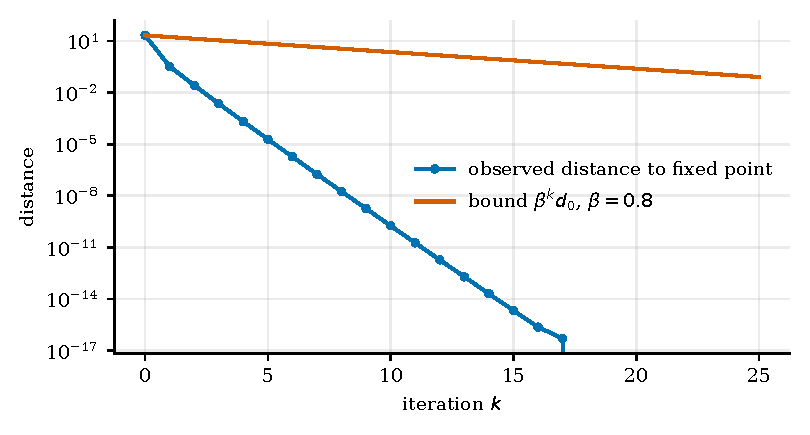
\includegraphics[width=0.85\textwidth]{figs/contraction}
\caption{Distance to the fixed point for the softmax update with $\beta=0.8$ on twelve unit traces in $\R^{64}$, with the bound $\beta^kd_0$ of Theorem~\ref{thm:contract}(i). Computed by the script \texttt{figs.py} with seed 8; an illustration of the stated analytic result and not an evaluation of the architecture.}\label{fig:contraction}
\end{figure}

\section*{Three traces: the Jacobian, the spectrum, and the loss of stability}\label{sec:three33}

The statements of Theorem~\ref{thm:contract} are easiest to appreciate when every quantity can be computed in closed form. The smallest store with a nontrivial competition among traces consists of three orthonormal traces, and this section works it through. Everything below is a worked example of results already proved, together with one extension, the expansion of the unstable branch near the threshold, which is derived here by a direct series computation.

\begin{workedex}[Three orthonormal traces]\label{ex:three33}
Let $m_1,m_2,m_3$ be the standard basis of $\R^3$ and consider the cue-free update $r\mapsto F(r)=\sum_iw_im_i$ with $w=\mathrm{softmax}(\beta r)$, so that $F(r)=w$ and the state lives on the probability simplex. By Chapter~\ref{ch:stability} the Jacobian at a point with weights $w$ is
\begin{equation}
J(w)=\beta\,\mathrm{Cov}_w(m)=\beta\bigl(\mathrm{diag}(w)-ww^{\top}\bigr),
\end{equation}
since $M^{\top}\mathrm{diag}(w)M=\mathrm{diag}(w)$ for orthonormal traces. At the uniform blend $w=(\tfrac13,\tfrac13,\tfrac13)$ the covariance has eigenvalues $\tfrac13,\tfrac13,0$, the zero belonging to the direction $(1,1,1)$ that leaves the simplex, so the Jacobian has leading eigenvalue $\beta/3$ and the blend is locally stable exactly when $\beta<3$, as Theorem~\ref{thm:contract}(ii) requires with $\lambda_{\max}(\mathrm{Cov})=\tfrac13$. Above that temperature the blend is unstable, and the question is where the iteration goes.

The other fixed points have the symmetric form $r=(a,b,b)$ with $a+2b=1$ and $t=a-b$. Substituting into $a=1/(1+2e^{-\beta t})$ gives the scalar equation
\begin{equation}\label{eq:three33}
t=\frac{1-e^{-\beta t}}{1+2e^{-\beta t}},
\end{equation}
whose solution $t=0$ is the uniform blend, $t>0$ is a state dominated by one trace and $t<0$ is a blend of two traces with the third suppressed. A series expansion about $t=0$ gives $\tfrac{1-e^{-\beta t}}{1+2e^{-\beta t}}=\tfrac{\beta t}{3}\bigl(1+\tfrac{\beta t}{6}+O(t^2)\bigr)$, hence \eqref{eq:three33} reads $t(1-\beta/3)=\tfrac{\beta^2}{18}t^2+O(t^3)$ and the nonzero branch near the threshold is
\begin{equation}
t\ \approx\ \frac{6(3-\beta)}{\beta^2},
\end{equation}
which changes sign at $\beta=3$. The bifurcation at $\beta=3$ is therefore transcritical and not a pitchfork, because the branch passes through the blend rather than emerging symmetrically from it. At $\beta=2.9$ the approximation gives $\ntbranchapprox$ and the exact root is $\ntlowCJ$.

Numerical solution of \eqref{eq:three33}, checked against the iteration itself, gives the following picture. For $\beta<\nonset$ the blend is the only fixed point, and for $\beta=2$ the equation has $\ncnttwo$ nonzero roots. At $\beta\approx\nonset$ a saddle-node creates a pair of positive roots. On the window $\nonset<\beta<3$ the blend (leading Jacobian eigenvalue $\nevblendCJ$ at $\beta=2.9$) and a one-trace state ($t=\nthighCJ$, leading eigenvalue $\nevhighCJ$) are both stable, separated by the unstable branch ($t=\ntlowCJ$, leading eigenvalue $\nevlowCJ$), so the system is bistable and the unstable fixed point lies on the boundary between the two basins. At $\beta=3$ the unstable branch meets the blend, which loses its stability there, and for $\beta>3$ the branch continues to $t<0$ as the family of two-trace blends.

At $\beta=6$ there are three kinds of fixed point besides the blend. The one-trace state $r=(\napos,\nbpos,\nbpos)$ has Jacobian eigenvalues $\nevposone$ and $\nevpostwo$ (and $0$ along the normal), so it is a contraction locally and an attractor. The two-trace blend $r=(\naneg,\naneg,\nbneg)$ has eigenvalues $\nevnegone$ and $\nevnegtwo$; the leading one is $\beta$ times the weight $\naneg$ on either of the two surviving traces, with eigenvector $(1,-1,0)$, and it exceeds one, so the blend is a saddle that separates the basins of the two traces it contains. The uniform blend has leading eigenvalue $\nevuniform=\beta/3$ and is repelling. The retrieval picture at high temperature is therefore three attractors, one per trace, separated by saddles at the pair blends and with a repeller at the center.
\end{workedex}

\begin{figure}[t]
\centering
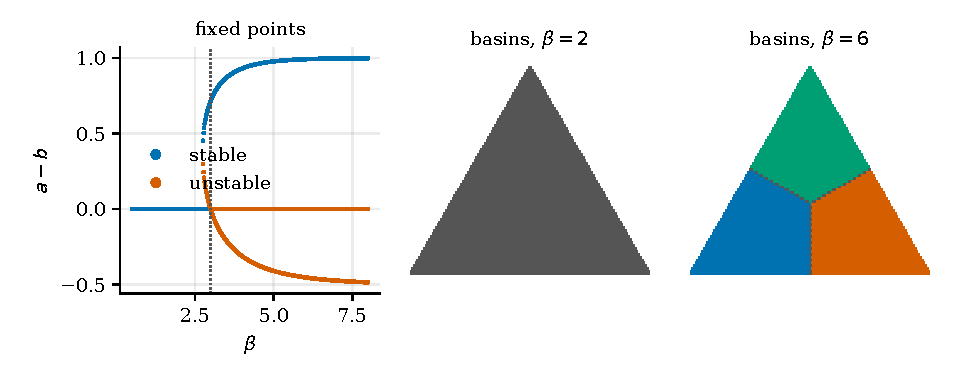
\includegraphics[width=\textwidth]{gen/three_trace}
\caption{The three-orthonormal-trace example. Left: fixed-point branches of \eqref{eq:three33}, expressed as the difference $a-b$, against $\beta$, with stable points in blue and unstable points in orange; the saddle-node near $\beta=\nonset$ and the crossing of the blend at $\beta=3$ are visible. Center and right: basins of attraction of the update on the probability simplex for $\beta=2$ and $\beta=6$. Below the threshold every initial state reaches the uniform blend (grey); above it the simplex divides into three basins. Computed by \texttt{examples.py} with a fixed seed; an illustration of the analytic result.}\label{fig:three33}
\end{figure}

The example shows what the threshold in Theorem~\ref{thm:contract} does and does not control. Crossing $\beta=3$ is the moment at which the blend ceases to be stable, but selection already becomes possible slightly earlier, on the bistable window, where the basin of the one-trace state grows from nothing. The theorem's condition $\beta\lambda_{\max}(\mathrm{Cov}_{w^\star})<1$ is evaluated at a fixed point, and the example shows that different fixed points of the same dynamics have different spectra, so a statement of the form ``the system is stable at temperature $\beta$'' is meaningless without naming the fixed point.

\begin{extension}[Overlap shifts the threshold]\label{ext:overlap33}
Let the three traces have pairwise overlap $\mu\in[0,1)$ and equal norms. By symmetry the blend $r=\bar m$ is still a fixed point with uniform weights, and the covariance of the traces under uniform weights has leading eigenvalue $(1-\mu)/3$. The blend is therefore stable if and only if $\beta<3/(1-\mu)$.
\end{extension}

\begin{proof}
The Gram matrix of the traces is $G=\mu\mathbf 1\mathbf 1^{\top}+(1-\mu)I$. For uniform weights $\mathrm{Cov}(m)=\tfrac13M^{\top}(I-\tfrac13\mathbf 1\mathbf 1^{\top})M$, whose nonzero eigenvalues coincide with those of $\tfrac13(I-\tfrac13\mathbf 1\mathbf 1^{\top})G$. On the subspace orthogonal to $\mathbf 1$ the matrix $G$ acts as $(1-\mu)I$, so the nonzero eigenvalue is $(1-\mu)/3$ with multiplicity two.
\end{proof}

For $\mu=\tfrac12$ the threshold is $\nthrmu$, and the numerical Jacobian at the blend has leading eigenvalue $\nevmuF$ at $\beta=5$ and $\nevmuH$ at $\beta=7$, so it crosses one between them as the formula predicts. The consequence is that correlation among traces postpones the onset of selectivity: the more the stored traces overlap, the colder the system must be, in the sense of a larger $\beta$, before the blend loses stability. This is the dynamical counterpart of the capacity statement of Chapter~\ref{ch:capacity}, that the number of distinguishable traces is controlled by the overlaps.


\chapter{Resonance Selectivity and Capacity}\label{ch:capacity}

The question of capacity is how many traces can be stored before retrieval degrades, and the answer depends on assumptions about the distribution of traces, the noise in the cue, and what counts as success. This chapter derives bounds under explicit assumptions. They are bounds under a random-pattern model and should not be read as measured properties of any particular dataset.

\paragraph{Random-pattern model.} Let the stored traces $m_1,\dots,m_P$ be independent and uniformly distributed on the unit sphere of $\C^n\cong\R^{2n}$. The cap estimate that underlies everything below is that for two independent uniform unit vectors the real overlap satisfies
\begin{equation}\label{eq:cap}
\Pr\bigl[\Re\ip{u}{v}\ge a\bigr]\le(1-a^2)^{n-1}\le e^{-(n-1)a^2},\qquad 0<a<1,
\end{equation}
which follows from the standard bound on the measure of a spherical cap \cite{ball1997}. Equation~\eqref{eq:cap} was verified numerically in the pilot calculations of Appendix~\ref{app:pilot} for $n\in\{16,32,64\}$.

\begin{proposition}[False activation under a resonance threshold]\label{prop:falseact}
Let $\psi,q$ be unit vectors in $\C^n$, so that by Theorem~\ref{thm:closed} the resonance score is $S(\psi,q)=\tfrac12\bigl(1+\Re\ip{\psi}{q}\bigr)$. If a trace is declared active when $S\ge\theta$ with $\theta\in(\tfrac12,1)$, then for a query $q$ independent of $P$ stored random unit traces, the expected number of false activations satisfies
\begin{equation}
\Ex[\#\text{active}]\le P\,e^{-(n-1)(2\theta-1)^2}.
\end{equation}
\end{proposition}

\begin{proof}
$S\ge\theta$ is equivalent to $\Re\ip{\psi}{q}\ge2\theta-1$. Apply \eqref{eq:cap} with $a=2\theta-1$ to each trace and sum over $P$ traces by linearity of expectation.
\end{proof}

The threshold needed to hold the expected number of false activations below one is therefore $2\theta-1\ge\sqrt{\ln P/(n-1)}$, which says that the usable score threshold rises toward one as the store grows at fixed dimension, and the capacity for a given threshold is exponential in the dimension, $P\le e^{(n-1)(2\theta-1)^2}$. This is the exponential capacity in the dimension that is characteristic of dense associative memories \cite{demircigil2017,ramsauer2021}, obtained here for the threshold readout, and its dependence on the squared margin shows the cost of lowering the threshold to tolerate degraded cues.

For the recurrent softmax readout the relevant event is that the stored traces are well separated, so that Proposition~\ref{prop:basin} applies.

The result that follows must be read for what it is. It is a capacity theorem for associative retrieval by a softmax readout over random unit vectors, and the exponential scaling is the familiar consequence of high-dimensional concentration together with a sufficiently low temperature \cite{demircigil2017,ramsauer2021}. It guarantees one-step proximity to a stored trace. It says nothing about recovering temporal organization, historical provenance, or an episode reconstructed from distributed constraints, and it should not be cited as establishing an exponential capacity for episodic recollection. Its role is to show that the retrieval component of the architecture can match known forms of high-dimensional pattern separation, and its price, a temperature that grows linearly with the dimension, is stated in the theorem.

\begin{theorem}[Baseline associative capacity of the softmax readout]\label{thm:capacity}
Let $P=e^{\kappa(n-1)}$ traces be drawn as above, and let $a\in(0,1)$ satisfy $a^2>2\kappa$. Then with probability at least $1-\tfrac12e^{(n-1)(2\kappa-a^2)}$ the maximum overlap satisfies $\max_{i\ne j}\Re\ip{m_i}{m_j}<a$. On this event, for every stored trace $m_j$ and every cue $r$ with $\norm r\le1$ and $\norm{r-m_j}\le\delta$ for some $\delta<(1-a)/2$, one update of the softmax map \eqref{eq:modernhop} with inverse temperature $\beta$ in the realified space satisfies
\begin{equation}
\norm{F(r)-m_j}\le2(P-1)\,e^{-\beta(1-a-2\delta)}.
\end{equation}
In particular the error is below any prescribed $\eta>0$ once $\beta(1-a-2\delta)\ge\kappa(n-1)+\ln(2/\eta)$.
\end{theorem}

\begin{proof}
There are $\binom P2\le P^2/2$ pairs, and the union bound with \eqref{eq:cap} gives the probability that some pair has overlap at least $a$ as at most $\tfrac12P^2e^{-(n-1)a^2}=\tfrac12e^{(n-1)(2\kappa-a^2)}$. On the complement, for the cue $r$ one has $\ip{m_j}{r}=1+\ip{m_j}{r-m_j}\ge1-\delta$ and, for $i\ne j$, $\ip{m_i}{r}=\ip{m_i}{m_j}+\ip{m_i}{r-m_j}\le a+\delta$. The margin is at least $\Delta=1-a-2\delta>0$, and Proposition~\ref{prop:basin} gives the stated bound with $\varepsilon\le(P-1)e^{-\beta\Delta}$. The final statement solves $2Pe^{-\beta\Delta}\le\eta$ for $\beta\Delta$ using $\ln P=\kappa(n-1)$.
\end{proof}

The theorem shows, for associative retrieval of stored traces and not for episodic reconstruction, that the number of recoverable traces can grow exponentially in the dimension, with the rate $\kappa<a^2/2$, provided the inverse temperature grows linearly with the dimension, $\beta\gtrsim\kappa(n-1)/(1-a-2\delta)$. The scaling of $\beta$ is the hidden cost: a memory sharp enough to store exponentially many traces is a memory whose Jacobian $\beta\Cov_w(m)$ is large away from the attractors, so its basins are narrow and its blend states unstable (Theorem~\ref{thm:contract}). Interference accumulates in a different manner under the dilution formula of Proposition~\ref{prop:dilution}: adding a competitor with score $s_n$ rescales the weight of every earlier trace by $Z/(Z+e^{\beta s_n})$, which is small only when the competitor's score is low relative to the incumbents' normalizer. The random-pattern model is the best case for capacity, because it makes overlaps small. Structured stores with clusters of near-duplicates have larger $\mu$ in Proposition~\ref{prop:basin} and require larger margins, and the correlated-pattern and phase-correlated cases are reserved for the experimental program of Chapter~\ref{ch:scaling}.

Figure~\ref{fig:captail} compares the cap bound \eqref{eq:cap} with simulation for three dimensions. The bound holds throughout and has the correct exponential dependence on $n$ and on $a^2$, which is what the capacity argument of Theorem~\ref{thm:capacity} uses.

\begin{figure}[t]
\centering
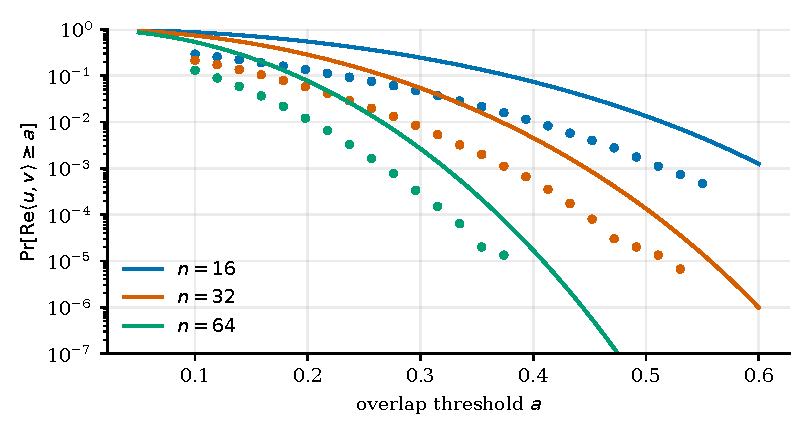
\includegraphics[width=0.85\textwidth]{figs/capacity_tail}
\caption{Empirical tail probability of the real overlap of two independent uniform unit vectors in $\C^n\cong\R^{2n}$ (points, $3\times10^5$ samples) with the cap bound $(1-a^2)^{n-1}$ (curves). Computed by the script \texttt{figs.py} with seed 8; an illustration of the stated analytic result and not an evaluation of the architecture.}\label{fig:captail}
\end{figure}

\section*{Why the margin hypothesis matters}\label{sec:margin34}

The guarantee of Proposition~\ref{prop:basin}, and through it Theorem~\ref{thm:capacity}, is conditional on a margin $\Delta$ between the cued trace and its competitors that exceeds $\beta^{-1}\ln(P-1)$. This section shows by example what happens when the hypothesis fails. It also separates two statements that are easily run together, namely that a sufficient condition has failed and that retrieval has failed. The second statement needs its own proof, and the examples give it by exact computation in a family where everything is available in closed form.

\begin{counterex}[Near-duplicate traces]\label{cex:margin34}
Take $P$ unit traces with a common pairwise overlap $\mu$, that is, with Gram matrix $G=\mu\mathbf 1\mathbf 1^{\top}+(1-\mu)I$, and cue with the first trace, $r=m_1$. The margin is $\Delta=1-\mu$ for every competitor, the weights are $w_1=\bigl(1+(P-1)e^{-\beta(1-\mu)}\bigr)^{-1}$ on the cued trace and $(1-w_1)/(P-1)$ on each other trace, and the one-step error is an exact expression,
\begin{equation}\label{eq:symerr}
\norm{F(m_1)-m_1}=(1-w_1)\sqrt{\frac{1+(P-2)\mu}{P-1}+1-2\mu},
\end{equation}
because $F(m_1)-m_1=(1-w_1)(\bar c-m_1)$ with $\bar c$ the centroid of the competitors. Consider $P=21$ and $\mu=0.9$. The weight on the cued trace equals one half exactly at
\begin{equation}
\beta^\ast=\frac{\ln(P-1)}{1-\mu}=\nbstar,
\end{equation}
and below this temperature the cued trace does not even carry a majority of the weight. At $\beta=20$ one finds $w_1=\nwoneCA$ and a one-step error of $\nerrsymCA$ against a distance $\ndistsym$ from $m_1$ to the centroid of its competitors, so most of the displacement toward the centroid has taken place. The bound of Proposition~\ref{prop:basin} reads $\varepsilon\le(P-1)e^{-\beta\Delta}=\nepsbCA$, which exceeds one and says nothing. At $\beta=40$ the weight is $\nwoneEA$, the error is $\nerrsymEA$ and the bound is $\nepsbEA<1$, so the hypothesis holds and the conclusion is informative. The figure shows the weight $w_1$ against $\beta$ for four store sizes together with the threshold $\ln(P-1)/(1-\mu)$ for each, which grows with the logarithm of the store.
\end{counterex}

\begin{figure}[t]
\centering
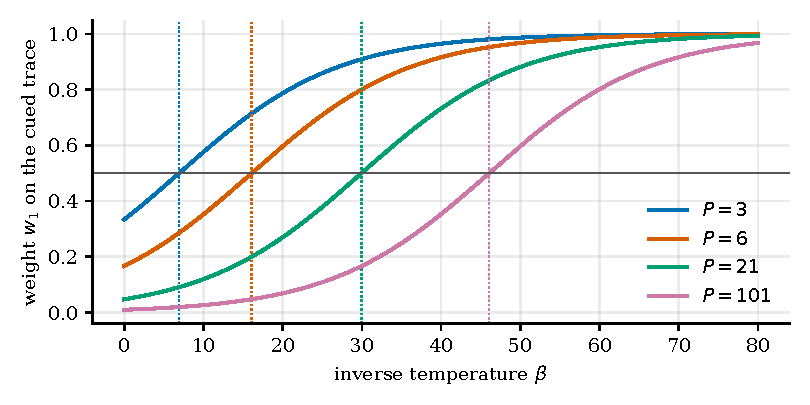
\includegraphics[width=0.85\textwidth]{gen/margin_threshold}
\caption{Weight on the cued trace against inverse temperature for the symmetric near-duplicate family with $\mu=0.9$ and $P\in\{3,6,21,101\}$. The dotted verticals mark $\beta^\ast=\ln(P-1)/(1-\mu)$, where the weight equals one half. Computed by \texttt{examples.py}; an illustration of the closed form in Counterexample~\ref{cex:margin34}.}\label{fig:margin34}
\end{figure}

The counterexample is stated as a necessary scale and not only as a failure. If the hypothesis $\beta\Delta>\ln(P-1)$ is violated by a symmetric family, then $w_1<\tfrac12$, so the single-step update moves the state further than halfway to the competitor centroid; the margin condition is therefore not an artifact of the proof but the temperature at which a symmetric cluster stops being resolved. The same expression also shows why sharpening the temperature is a costly remedy. For this family the cue-free iteration $r\mapsto F(r)$ started at $m_1$ converges for every $\beta$ tested (from $10$ to $40$) to the uniform blend, at distance $\nblendfpdist$ from $m_1$, because the blend remains stable until $\beta$ reaches $1/\lambda_{\max}=P/(1-\mu)=\nblendthr$, where $\lambda_{\max}=(1-\mu)/P$ is the leading covariance eigenvalue at uniform weights, the computation of Extension~\ref{ext:overlap33} with $P$ in place of three. In a store of near-duplicates the temperature at which the cue-free iteration becomes selective is therefore much higher than the temperature at which one step resolves the cue, and whether a cue-anchored iteration of the type in Proposition~\ref{prop:map} holds the cued trace in this regime is not decided by the computation above.

\begin{counterex}[A vacuous bound without a failed retrieval]\label{cex:vacuous34}
A conclusion that the proposition cannot certify is not a conclusion that is false. Take two traces with overlap $\mu=0.9$, so $\norm{m_1-m_2}=\ntwodist$, cue with $r=m_1$ and let $\beta=10$. The margin is $\Delta=0.1$, and the bound of Proposition~\ref{prop:basin} is $\norm{F(r)-m_1}\le2(P-1)e^{-\beta\Delta}=\ntwobound$. This exceeds the distance $\ntwodist$ between the two traces, which is the largest displacement possible for a convex combination of them, so the bound is vacuous. The exact computation gives a weight $\ntwow$ on the competitor and a one-step error $\ntwoerr$, nearly four times smaller than the distance between the traces. The output is closer to $m_1$ than to $m_2$, so the retrieval selects the right trace even though the proposition certifies nothing.
\end{counterex}

The two counterexamples together state what the margin hypothesis can and cannot be used for. Counterexample~\ref{cex:vacuous34} shows that a margin too small to make the bound informative is compatible with correct identification of the nearest trace. Counterexample~\ref{cex:margin34} shows that small margins are not harmless either: in the near-duplicate family the uninformative regime coincides with an exactly computed one-step error comparable to the whole displacement toward the competitor centroid, and with a drift of the cue-free iteration to the blend. The logical situation is that Proposition~\ref{prop:basin} is a sufficient condition, so an uninformative bound licenses no inference by itself, and a conclusion of retrieval failure must be supported by a separate computation, as it is in \eqref{eq:symerr}. For this reason the experimental program of Part~IX reports the margin and the observed error together and does not treat the margin as a predictor.


\chapter{Information Geometry of Memory}\label{ch:geometry}

A memory read out through a softmax or through a Bayesian posterior produces, for each cue, a probability distribution over traces or latent causes. The information geometry of these distributions provides a language for distinguishability that does not depend on the coordinates of the stored embeddings. This chapter develops the elementary parts of that language and states plainly what they do and do not establish.

The softmax weights form an exponential family indexed by the inverse temperature: $p_\beta(i\mid r)=\exp(\beta s_i-\Lambda(\beta))$ with $s_i=\ip{m_i}{r}$ and log-partition $\Lambda(\beta)=\ln\sum_je^{\beta s_j}$. For an exponential family the Fisher information for the natural parameter is the variance of the sufficient statistic, so that
\begin{equation}\label{eq:fishertemp}
\mathcal I(\beta)=\Var_{w}(s)=\Lambda''(\beta),
\end{equation}
which is the amount of information that a single draw of the selected trace carries about the temperature, and which is zero for every $\beta$ if the scores are all equal, tends to zero as $\beta\to\infty$ when the weights collapse onto one trace, and at $\beta=0$ equals the variance of the scores under uniform weights. It can therefore peak at an intermediate temperature where several traces compete, as the example below shows, but it need not do so: the location of the maximum depends on the score profile. This has a consequence for the identifiability analysis of Chapter~\ref{ch:precision}: precision and temperature can be distinguished from outcomes only where this variance is nonzero, and the cue-specific manipulations that make it nonzero are the ones that identify precision.

The space of distributions over a finite set carries a canonical metric, the Fisher--Rao metric $g(\dot p,\dot p)=\sum_i\dot p_i^2/p_i$. The substitution $u_i=2\sqrt{p_i}$ maps the open simplex isometrically onto the positive orthant of the sphere of radius two, since $du_i=dp_i/\sqrt{p_i}$ gives $\sum_idu_i^2=\sum_idp_i^2/p_i$. The geodesic distance is therefore
\begin{equation}\label{eq:fr}
d_{FR}(p,q)=2\arccos\mathrm{BC}(p,q),\qquad\mathrm{BC}(p,q)=\sum_i\sqrt{p_iq_i},
\end{equation}
where $\mathrm{BC}$ is the Bhattacharyya coefficient. The metric is, up to scale, the only Riemannian metric on the simplex that is invariant under sufficient statistics, a theorem of \v{C}encov that is the usual justification for calling it canonical \cite{amari2016}. The geometry reflects the fact that the probability of confusing two distributions from finite samples is controlled by $\mathrm{BC}$, with large $\mathrm{BC}$ meaning near-indistinguishability.

The monotonicity property of this geometry gives a clean bound on what can be recovered from a posterior.

\begin{proposition}[Data-processing for recollective distinguishability]\label{prop:dpi}
Let $K$ be a stochastic kernel from a finite set $\mathcal X$ to a finite set $\mathcal Y$, and let $p,q$ be distributions on $\mathcal X$. Then $\mathrm{BC}(pK,qK)\ge\mathrm{BC}(p,q)$, and consequently $d_{FR}(pK,qK)\le d_{FR}(p,q)$.
\end{proposition}

\begin{proof}
For each $y$, the Cauchy--Schwarz inequality gives
\begin{equation*}
\sqrt{\Bigl(\sum_xp_xK_{xy}\Bigr)\Bigl(\sum_xq_xK_{xy}\Bigr)}\ \ge\ \sum_x\sqrt{p_xq_x}\,K_{xy}.
\end{equation*}
 Summing over $y$ and using $\sum_yK_{xy}=1$ gives the first inequality, and the second follows because $\arccos$ is decreasing.
\end{proof}

If the cues $c$ and $c'$ induce posteriors $p_c$ and $p_{c'}$ over latent causes of Chapter~\ref{ch:inference}, and the reconstruction is a stochastic function of the cause, then the distributions of reconstructions satisfy the proposition's bound: two cues whose posteriors are close in the Fisher--Rao metric cannot produce reconstructions that are further apart in that metric. The geometry of posteriors thus bounds the distinguishability of recollections from above. The proposition does not say that the geometry of posteriors characterizes accessibility, since it is silent about the computational cost of realizing the kernel, and it does not remove the dependence on the stored embeddings, since the posteriors are computed from them. Whether accessibility admits a characterization in terms of the posterior geometry alone, rather than a bound, is left as Problem~\ref{prob:geometry}.

\begin{workedex}[Fisher information of the temperature and a data-processing check]\label{ex:fisher35}
Take three traces with scores $s=(1.0,\,0.2,\,0)$ against a cue. The Fisher information $\mathcal I(\beta)=\mathrm{Var}_w(s)$ equals $\nfishA$ at $\beta=0$, where the weights are uniform, rises to a maximum of $\nfishpeak$ near $\beta=\nfishpeakb$, and falls to $\nfishDA$ (to four decimals) at $\beta=30$, where the first trace carries essentially all the weight. A numerical second difference of the log-partition function reproduces $\mathcal I(\beta)$ to within $10^{-5}$ at $\beta\in\{0.5,3,10\}$, which checks \eqref{eq:fishertemp}. The practical consequence is the one stated above: a cue of this kind identifies the temperature only in an intermediate band, and the design of a cue family for identifying precision is the design of score profiles whose variance is large where the system is meant to operate. A different profile, for instance $(0.9,0.5,0.1)$, has its maximum at $\beta=0$, which is why the location of the peak cannot be asserted in general.

For the distances, let $p=(0.5,0.3,0.2)$ and $q=(0.2,0.3,0.5)$ be the posteriors over three latent causes induced by two cues, and let the reconstruction be a stochastic function of the cause through the kernel with rows $(0.9,0.1)$, $(0.5,0.5)$ and $(0.1,0.9)$. Then $\mathrm{BC}(p,q)=\nBCbefore$ and $d_{FR}(p,q)=\ndFRbefore$, while the output laws satisfy $\mathrm{BC}(pK,qK)=\nBCafter$ and $d_{FR}(pK,qK)=\ndFRafter$. The distance has shrunk, as Proposition~\ref{prop:dpi} requires, and the shrinkage quantifies how much of the distinction between the two cues is lost by the stochastic reconstruction.
\end{workedex}

\begin{problem}[Geometric characterization of accessibility]\label{prob:geometry}
Define a family of cost-bounded decoders and the induced notion of accessible recollective equivalence. Determine whether the equivalence classes of accessible equivalence are the level sets of a function of the Fisher--Rao geometry of the posteriors $\{p_c\}$ alone, or whether the cost of the decoder introduces invariants of the representation that the posterior geometry does not capture.
\end{problem}

\chapter{Projection, Abstraction, and Sufficient Memory States}\label{ch:projection}

An abstraction is a map $\pi:\mathcal X\to\bar{\mathcal X}$ from detailed memory states to compressed representations. For a deterministic dynamics $F:\mathcal X\to\mathcal X$ the abstraction is dynamically adequate if the compressed state evolves autonomously, that is, if there is a map $\bar F$ on the compressed space with
\begin{equation}\label{eq:commute}
\pi\circ F=\bar F\circ\pi.
\end{equation}

\begin{proposition}[Closure criterion]\label{prop:closure}
A map $\bar F$ satisfying \eqref{eq:commute} exists if and only if $\pi(x)=\pi(y)$ implies $\pi(F(x))=\pi(F(y))$, that is, if the kernel equivalence of $\pi$ is preserved by $F$. When it exists it is unique on $\pi(\mathcal X)$.
\end{proposition}

\begin{proof}
If \eqref{eq:commute} holds and $\pi(x)=\pi(y)$ then $\pi(F(x))=\bar F(\pi(x))=\bar F(\pi(y))=\pi(F(y))$. Conversely, if the implication holds define $\bar F(\pi(x))=\pi(F(x))$, which is well defined by hypothesis.
\end{proof}

For stochastic dynamics the same criterion is the strong lumpability of Proposition~\ref{prop:accmarkov}. The criterion is about closure of the projected dynamics, and closure alone says nothing about whether the projection keeps what a recollection needs. The following example separates the two ideas.

\begin{example}[Closure without sufficiency]\label{ex:trivialproj}
Take any $F$ and the projection $\pi(x)=0$ onto a single point. Then $\bar F(0)=0$ satisfies \eqref{eq:commute}, and the compressed dynamics is trivially closed. It also discards every distinction among states, so no nonconstant target can be recovered. Conversely, the identity projection preserves everything and is closed, but achieves no compression. A projection that is useful must be closed and must keep the equivalence class that the future queries require.
\end{example}

\begin{proposition}[Closure and sufficiency together answer future queries]\label{prop:closeandsuff}
Suppose $\pi\circ F=\bar F\circ\pi$ and the reconstruction factors through the projection, $\Eph(x,c)=\bar\Eph(\pi(x),c)$. Then for every initial state $x_0$, every number of steps $k$ and every cue $c$, the reconstruction after $k$ steps equals $\bar\Eph(\bar F^k(\pi(x_0)),c)$, so the compressed system answers every query that the detailed system answers along the trajectory.
\end{proposition}

\begin{proof}
By induction, $\pi(F^k(x_0))=\bar F^k(\pi(x_0))$, since $\pi(F^{k+1}(x_0))=\bar F(\pi(F^k(x_0)))$. Then $\Eph(F^k(x_0),c)=\bar\Eph(\pi(F^k(x_0)),c)$.
\end{proof}

Exact closure is rare and approximate closure is the realistic notion. Suppose the commutation defect is bounded, $\norm{\pi F(x)-\bar F\pi(x)}\le\varepsilon$ for all $x$, and $\bar F$ is $\bar L$-Lipschitz. Let $x_k=F^k(x_0)$ and $\bar x_k=\bar F^k(\pi(x_0))$.

\begin{proposition}[Drift under approximate commutation]\label{prop:drift2}
Under these assumptions $\norm{\pi(x_k)-\bar x_k}\le\varepsilon\sum_{j=0}^{k-1}\bar L^{\,j}$, which is $\varepsilon(1-\bar L^{k})/(1-\bar L)$ for $\bar L\ne1$ and $k\varepsilon$ for $\bar L=1$.
\end{proposition}

\begin{proof}
Let $e_k=\norm{\pi(x_k)-\bar x_k}$, with $e_0=0$. Then $e_{k+1}\le\norm{\pi F(x_k)-\bar F\pi(x_k)}+\norm{\bar F\pi(x_k)-\bar F(\bar x_k)}\le\varepsilon+\bar Le_k$, and the stated sum follows by induction.
\end{proof}

The compressed model is therefore reliable on a horizon of order $1/\varepsilon$ when $\bar L\ge1$, and on all horizons, with error at most $\varepsilon/(1-\bar L)$, when the compressed dynamics is a contraction. The qualitative implication, that contractive compressed dynamics tolerate imperfect closure indefinitely while expansive dynamics do not, bears on the design of consolidation: the slow store of Chapter~\ref{ch:consolidation} should have contractive replay dynamics if it is to remain a faithful abstraction of the fast store.

\paragraph{A linear example: projection onto the span of the traces.}
The projection that discards cue components orthogonal to the traces is an instance of closure that can be checked exactly. Let $V=\operatorname{span}\{m_1,\dots,m_P\}\subset\R^N$ and let $\Pi$ be the orthogonal projector onto $V$. Because each $m_i\in V$, the scores satisfy $\ip{m_i}{r}=\ip{m_i}{\Pi r}$ for every $r$, so the softmax weights depend on $r$ only through $\Pi r$, and the update obeys
\begin{equation}\label{eq:blind}
F(r)=F(\Pi r),\qquad F(r)\in\operatorname{conv}\{m_i\}\subset V,\qquad\text{hence}\qquad \Pi F=F=F\Pi.
\end{equation}
The projection $\pi=\Pi$ is therefore exactly closed with $\bar F=F|_V$, and the update is blind to the component of the cue normal to $V$. If the cue is corrupted by isotropic noise $\xi$ with $\Ex[\xi\xi^\top]=\sigma^2 I_N$, then $\Ex\norm{\Pi\xi}^2=\sigma^2\dim V$, so the fraction of the noise energy that survives the projection is $\dim V/N$, and the remaining fraction $1-\dim V/N$ is removed in one step. When the stored traces span a low-dimensional subspace of a high-dimensional ambient space, most of the noise is discarded.

This is the linear counterpart of the tangent--normal decomposition developed in the author's companion manuscripts on manifold-aligned prediction \cite{flyxion2026npn,flyxion2026hall}. In that framework the semantic manifold $\mathcal M$ has at each point a tangent space and its orthogonal complement, the normal space; admissible explanatory updates lie in the tangent space, and components of an update in the normal space are those that depart from the lawful structure of the data, which the companion work identifies with hallucination. The span $V$ here is the globally flat special case in which the tangent space is the same at every point and the normal space is its complement. Equation~\eqref{eq:blind} says that Mem8's softmax reconstruction has the no-normal-component property in this special case by construction, so that normal-direction content in an output could only enter through additive noise in the dynamics or from a decoder that is not the softmax readout. The curved case requires local tangent spaces and a projection that depends on the base point, and neither the closure property nor the noise-removal fraction extends to it without curvature corrections; those extensions are stated in the companion work and are not derived here. The claims of the companion manuscripts concerning the empirical behavior of recent generative models are cited as claims of those manuscripts and not asserted independently.

Figure~\ref{fig:noise} checks the linear tangent--normal statement of equation \eqref{eq:blind}. The fraction of noise energy surviving the projection matches $\dim V/N$, so a trace span of low dimension discards most of an isotropic perturbation in one step.

\begin{figure}[t]
\centering
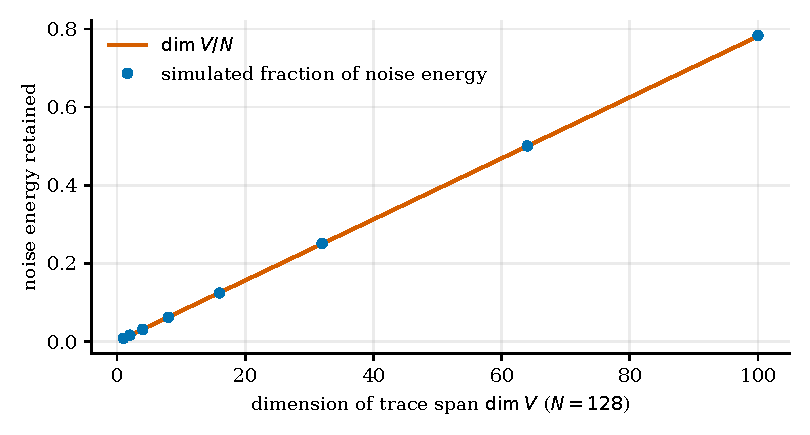
\includegraphics[width=0.85\textwidth]{figs/noise_removal}
\caption{Fraction of isotropic noise energy retained by projection onto the span of the traces in $\R^{128}$, against the dimension of the span, with the value $\dim V/N$ of equation \eqref{eq:blind}. In each run the softmax update was verified numerically to satisfy $F(r)=F(\Pi r)$. Computed by the script \texttt{figs.py} with seed 8; an illustration of the stated analytic result and not an evaluation of the architecture.}\label{fig:noise}
\end{figure}

\section*{Two ways to fail: closure without sufficiency and sufficiency without closure}\label{sec:twofail36}

Example~\ref{ex:trivialproj} separates closure from sufficiency with a degenerate projection that keeps nothing. Two finite constructions make the separation in both directions with projections that are nontrivial, and a stochastic version places it in the language of transition kernels. These are worked examples and a proposed extension; the criteria they exercise are Propositions~\ref{prop:closure} and~\ref{prop:accmarkov} and Theorem~\ref{thm:suff}.

\begin{counterex}[Closed but not sufficient]\label{cex:closedinsuff}
Let $\mathcal X=\{1,2,3,4\}$ with the dynamics $F$ that swaps within the pairs, $F(1)=2$, $F(2)=1$, $F(3)=4$, $F(4)=3$, and let $\pi$ identify each pair, $\pi(1)=\pi(2)=\mathsf A$ and $\pi(3)=\pi(4)=\mathsf B$. Then $\pi(x)=\pi(y)$ implies $\pi(F(x))=\pi(F(y))$, so by Proposition~\ref{prop:closure} the projection is closed, and in fact $\bar F$ is the identity on $\{\mathsf A,\mathsf B\}$. Let the target be the parity of the state within its pair, $T(1)=T(3)=1$ and $T(2)=T(4)=0$. The projection is not sufficient for $T$ by Theorem~\ref{thm:suff}, because the class $\{1,2\}$ contains states with different targets, and the failure is robust: no decoder that sees only the compressed state can answer the parity query at any time, since the compressed trajectory is constant and carries no information about it. The distinction destroyed by $\pi$ is dynamically invisible, which is exactly why closure does not detect its loss. The compressed system is a perfect autonomous model of the block label and an uninformative memory for the parity.
\end{counterex}

\begin{counterex}[Sufficient now but not closed]\label{cex:sufficientnotclosed}
Let $\mathcal X=\{1,2,3,4\}$ with $F(1)=3$, $F(2)=1$, $F(3)=3$, $F(4)=4$, let $T(1)=T(2)=1$ and $T(3)=T(4)=0$, and take the projection $\pi=T$, which has classes $\{1,2\}$ and $\{3,4\}$. The projection is sufficient for $T$ by construction, since the reconstruction is the label itself. It is not closed: $\pi(1)=\pi(2)$ but $\pi(F(1))=\pi(3)=0$ while $\pi(F(2))=\pi(1)=1$. Consequently the compressed system cannot predict its own future label from its present one. The same failure is visible in the language of recollection: the target after one update is $T\circ F$ with $T(F(1))=0$ and $T(F(2))=1$, so $\pi$ is not sufficient for $T\circ F$, and a memory that is sufficient for the recollections required today is not sufficient for the recollections required after one step of its own dynamics.
\end{counterex}

The two counterexamples correspond to two independent defects. Closure is a property of the pair $(\pi,F)$ and says that the kernel of $\pi$ is a congruence for $F$. Sufficiency is a property of the pair $(\pi,T)$ and says that the kernel of $\pi$ refines $\approx_T$. A projection supports recollection along a trajectory only when the kernel of $\pi$ refines $\approx_{T\circ F^k}$ for every $k$ in the horizon, and the coarsest such kernel is the congruence refinement of the targets, which Extension~\ref{ext:viabequiv} of Chapter~\ref{ch:viability} constructs for a system with inputs. The first counterexample shows that closure is not enough and the second that sufficiency at one time is not enough.

For a stochastic dynamics the same two properties are statements about kernels and conditional laws. Let $P$ be a transition kernel on a finite set $\mathcal X$, let $\pi$ partition $\mathcal X$ into blocks, and let $L(x,B')=\sum_{y\in B'}P(x,y)$ be the lumped row. The partition is strongly lumpable if $L(x,\cdot)$ depends on $x$ only through $\pi(x)$, in which case the lumped kernel $\bar P(\pi(x),\cdot)=L(x,\cdot)$ is the transition kernel of $\pi(X_k)$ for every initial law, which is Proposition~\ref{prop:accmarkov}. Sufficiency for a target $T$ at time $k$ is the statement that the conditional law of $T(X_k)$ given $\pi(X_k)$ is degenerate, which is equivalent to the vanishing of the Bayes risk of Extension~\ref{ext:bayesrisk} with the memory state $\pi(X_k)$ and the history $X_k$.

\begin{workedex}[A four-state chain that is lumpable and uninformative]\label{ex:lumped36}
Let $\mathcal X=\{0,1,2,3\}$ with blocks $\{0,1\}$ and $\{2,3\}$, and let the kernel have rows $(0.35,0.35,0.15,0.15)$ for states $0$ and $1$ and $(0.10,0.10,0.40,0.40)$ for states $2$ and $3$. The lumped rows are equal within each block, so the partition is strongly lumpable, with $\bar P=\begin{psmallmatrix}\npbaraa&0.30\\0.20&0.80\end{psmallmatrix}$. The target is the identity of the state within its block, $T(x)=x \bmod 2$. From the uniform initial law the law after one step is $(0.225,0.225,0.275,0.275)$. Given the block label, the two members of each block are equally likely, so the Bayes risk of the parity query is $\nriskblock$, which is the worst possible for a binary target, whereas given the full state it is zero. The compressed chain is therefore an exact autonomous model of the block process and carries no information whatever about the target; the closure of the lumped kernel and the insufficiency of the lumped state hold simultaneously, the stochastic form of Counterexample~\ref{cex:closedinsuff}.
\end{workedex}

Exact lumpability is also fragile, and the realistic notion is the approximate one. For the stochastic case the drift bound of Proposition~\ref{prop:drift2} takes the following form, in which the Lipschitz constant of the compressed dynamics is replaced by the Dobrushin contraction coefficient $\kappa(\bar P)=\max_{a,b}\mathrm{TV}(\bar P(a,\cdot),\bar P(b,\cdot))$.

\begin{extension}[Drift under approximate lumpability]\label{ext:lumpdrift}
Let $P$ be a kernel on a finite set with a partition $\pi$, and let $\bar P$ be a kernel on the blocks with defect $\varepsilon=\max_x\mathrm{TV}\bigl(L(x,\cdot),\bar P(\pi(x),\cdot)\bigr)$. Let $\nu_k$ be the law of $\pi(X_k)$ under $P$ from any initial law of $X_0$, and let $\bar\nu_k=\bar\nu_{k-1}\bar P$ with $\bar\nu_0=\nu_0$. Then
\begin{equation}
\mathrm{TV}(\nu_k,\bar\nu_k)\ \le\ \varepsilon\sum_{j=0}^{k-1}\kappa^j\ =\ \varepsilon\,\frac{1-\kappa^k}{1-\kappa}\ \le\ k\varepsilon,\qquad \kappa=\kappa(\bar P),
\end{equation}
with the middle expression read as $k\varepsilon$ if $\kappa=1$.
\end{extension}

\begin{proof}
Let $\mu_k$ be the law of $X_k$ and $e_k=\mathrm{TV}(\nu_k,\bar\nu_k)$, so $e_0=0$. Then $\nu_{k+1}=\sum_x\mu_k(x)L(x,\cdot)$, and the triangle inequality gives
\begin{equation}
e_{k+1}\le\mathrm{TV}\Bigl(\sum_x\mu_k(x)L(x,\cdot),\ \sum_x\mu_k(x)\bar P(\pi(x),\cdot)\Bigr)+\mathrm{TV}(\nu_k\bar P,\bar\nu_k\bar P)\le\varepsilon+\kappa\,e_k,
\end{equation}
since the middle term is an average of per-state defects and $\sum_x\mu_k(x)\bar P(\pi(x),\cdot)=\nu_k\bar P$, and since $\bar P$ contracts total variation by at most the Dobrushin coefficient. Induction from $e_0=0$ gives the claim.
\end{proof}

\begin{workedex}[Drift in a perturbed chain]\label{ex:drift36}
Perturb state $1$ of Worked Example~\ref{ex:lumped36} to the row $(0.29,0.35,0.21,0.15)$. Its lumped row becomes $(0.64,0.36)$ and the defect against the reference rows of the unperturbed states is $\varepsilon=\ndefect$. The Dobrushin coefficient of the reference kernel is $\kappa=\nkappa$. Starting in the perturbed state, the observed total variation distance between the true block law and the compressed prediction is $\ntvkF$ at $k=5$, against the bound $k\varepsilon=\nbndF$ and the sharper bound $\varepsilon(1-\kappa^k)/(1-\kappa)=\nbndFd$, and it settles at $\ntvinf$ at long horizons. The sharper bound is the informative one: because the compressed kernel contracts, errors do not accumulate linearly, and the asymptotic bound is $\varepsilon/(1-\kappa)=0.12$. The figure shows both bounds against the observed distance.
\end{workedex}

\begin{figure}[t]
\centering
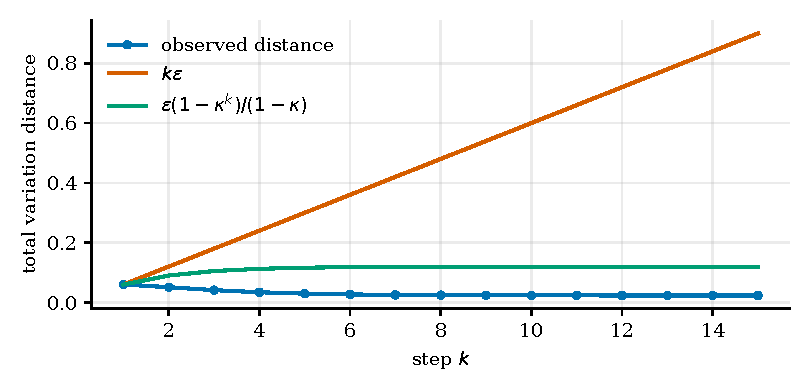
\includegraphics[width=0.85\textwidth]{gen/lump_drift}
\caption{Total variation distance between the true block law and the compressed prediction for the perturbed four-state chain of Worked Example~\ref{ex:drift36}, with the bounds $k\varepsilon$ and $\varepsilon(1-\kappa^k)/(1-\kappa)$ of Extension~\ref{ext:lumpdrift}. Computed by \texttt{examples.py}; an illustration of the stated bound.}\label{fig:lump36}
\end{figure}

The point of the pair of results is the separation of the roles. The bound controls how well the compressed state tracks the block process, which is closure. It does not control what the block process can say about the target, which is sufficiency and has to be certified by the separate criterion of Theorem~\ref{thm:suff}, or by its noisy form in Extension~\ref{ext:bayesrisk}. A system can have an excellent drift bound and a useless memory, as in Worked Example~\ref{ex:lumped36}, or a sufficient memory with an uncontrolled drift, as in Counterexample~\ref{cex:sufficientnotclosed}.


\chapter{Memory as Preservation of Viable Continuation}\label{ch:viability}

A memory is useful when it keeps the system's future options open under its objectives. Stated precisely, a memory policy is a rule that chooses encoding, update and release actions, and its quality is measured by the trajectories it makes possible. Let $f:\mathcal X\times\mathcal A\to\mathcal X$ be a deterministic transition law (stochastic versions replace membership by probability), let $K\subseteq\mathcal X$ be a set of admissible states, and call a trajectory viable if it remains in $K$ for all time.

\begin{definition}[Viability kernel]\label{def:viab}
The viability kernel of $K$ is the set $\Viab(K)$ of initial states from which some sequence of actions yields a trajectory remaining in $K$ forever.
\end{definition}

In the memory setting $K$ encodes constraints such as sufficient remaining resources, bounded interference, and, centrally, a floor on historical fidelity. Define a fidelity functional $D_t\ge0$ measuring the distortion of historically warranted reconstruction, and let $K=\{x:D(x)\le\delta\}\cap K_B$ where $K_B$ collects the resource constraints. The idealized objective of the proposal is
\begin{equation}\label{eq:objective}
\max_{\pi}\ \Ex_\pi\Bigl[\sum_{t=0}^\infty\gamma^t\bigl(U_t-\lambda C_t-\mu D_t\bigr)\Bigr],
\end{equation}
with $U_t$ the continuation value, $C_t$ the computational cost and $D_t$ the distortion. The structure of \eqref{eq:objective} is a penalized formulation in which fidelity trades against utility at the exchange rate $\mu$, and this is exactly what the monograph argues against making the only treatment of fidelity.

\begin{proposition}[Penalties cannot guarantee fidelity]\label{prop:penalty}
Suppose an action $a^\dagger$ yields per-step utility $G$ above the alternative at the cost of per-step distortion $d>\delta$, with all other terms equal. Then the penalized objective \eqref{eq:objective} prefers $a^\dagger$ whenever $\mu<G/d$ (using it at every step), whereas the constrained formulation, which requires the trajectory to stay in $K$, never selects it. For any fixed $\mu$ there exist utility gains $G>\mu d$ at which the penalized optimizer violates the fidelity bound.
\end{proposition}

\begin{proof}
Per step the penalized value of $a^\dagger$ relative to the alternative is $G-\mu d$, which is positive exactly when $\mu<G/d$, and discounting multiplies both sides by $\sum_t\gamma^t$. Under the constrained formulation $a^\dagger$ produces $D=d>\delta$ and leaves $K$, so it is infeasible. Given $\mu$, take $G>\mu d$.
\end{proof}

The proposition is simple, and it shows that with a finite penalty weight the guarantee of fidelity depends on the scale of the utilities, which are not controlled. A hard constraint is a different mathematical object, and its natural solution concept is the viability kernel. For a finite state space the kernel can be computed.

\begin{proposition}[Computation of the viability kernel]\label{prop:viabcomp}
Let $\mathcal X$ be finite and $\mathcal A$ finite. Define $K_0=K$ and $K_{j+1}=\{x\in K_j:\exists a\in\mathcal A,\ f(x,a)\in K_j\}$. The sequence is decreasing, stabilizes after at most $|K|$ steps at a set $K_\infty$, and $K_\infty=\Viab(K)$.
\end{proposition}

\begin{proof}
Each $K_{j+1}\subseteq K_j$, and since the sets are finite the sequence stops decreasing after at most $|K|$ strict decreases; at stabilization every $x\in K_\infty$ has an action leading to $K_\infty$, so repeating the choice yields a viable trajectory and $K_\infty\subseteq\Viab(K)$. Conversely, a state in $\Viab(K)$ has a viable trajectory, and by induction on $j$ every state of that trajectory lies in $K_j$ for all $j$, so $\Viab(K)\subseteq K_\infty$.
\end{proof}

A memory policy that respects the fidelity constraint is one that acts only within $\Viab(K)$, and the operational use of the kernel is to mark actions that appear beneficial in the short run but leave the viable set. For example, a release action that discards a trace is admissible only if the post-release state remains in the kernel, which requires that the discarded distinctions are not needed by any future cue in the committed family, in the sense of Theorem~\ref{thm:suff}. The constrained problem is then to maximize $\Ex\sum_t\gamma^t(U_t-\lambda C_t)$ over policies that stay in $\Viab(K)$, with fidelity a constraint and not a price. Historical fidelity remains separately measurable throughout, which is the property that allows the system to report that a useful reconstruction is historically unwarranted instead of silently trading one for the other.

\section*{Viability-preserving ecphoric equivalence}\label{sec:viabequiv37}

Theorem~\ref{thm:suff} asks which histories a memory must distinguish for the recollections required now, and Proposition~\ref{prop:viabcomp} asks which states the system must be able to leave through an admissible action. The two questions meet in a single one. Two memory states may be indistinguishable to every present recollection and to the present constraint, and yet respond differently once the memory is updated. Whether they may be merged depends on the family of admissible updates, and the answer is a quotient that is in general finer than the sufficiency quotient and coarser than the identity. This section constructs it and states exactly what is new and what is classical.

\paragraph{Setting.} Let $\Sigma=(\mathcal X,\mathcal A,f,K,T)$ be a deterministic system with finitely many memory states $\mathcal X$, a finite set $\mathcal A$ of admissible memory updates (consolidation steps, revisions, searches, releases), a transition law $f:\mathcal X\times\mathcal A\to\mathcal X$, an admissible set $K\subseteq\mathcal X$ and a present recollection map $T:\mathcal X\to\Recs$. Write $o(x)=(T(x),\mathbf 1_K(x))$ for the joint observation of the present recollection and the present admissibility, and $f_w(x)$ for the state reached by the action word $w\in\mathcal A^\ast$.

\begin{definition}[Viability-preserving ecphoric equivalence]\label{def:viabequiv}
Define $x\sim_0y$ if $o(x)=o(y)$ and $x\sim_{n+1}y$ if $x\sim_ny$ and $f(x,a)\sim_nf(y,a)$ for every $a\in\mathcal A$. The relation $\sim_\infty=\bigcap_n\sim_n$ is the viability-preserving ecphoric equivalence.
\end{definition}

\begin{extension}[Viability-preserving ecphoric equivalence]\label{ext:viabequiv}
For finite $\mathcal X$ the following hold. \emph{(i)} The chain $\sim_0\supseteq\sim_1\supseteq\cdots$ stabilizes after at most $|\mathcal X|-1$ refinements, and $\sim_\infty$ is the coarsest equivalence that refines $\sim_0$ and is a congruence for every $f(\cdot,a)$. \emph{(ii)} $x\sim_\infty y$ if and only if $o(f_w(x))=o(f_w(y))$ for every action word $w$; that is, the two states agree on every future recollection and on every future admissibility along every admissible sequence of updates. \emph{(iii)} The viability kernel $\mathrm{Viab}(K)$ of Definition~\ref{def:viab}, its robust counterpart $\{x:f_w(x)\in K\ \forall w\}$, and every set of the form $\{x: T(f_w(x))\in S\}$ are unions of $\sim_\infty$ classes. \emph{(iv)} An encoding $E:\mathcal X\to\Mem$ supports a decoder for $T\circ f_w$ and for $\mathbf 1_K\circ f_w$ for every word $w$ if and only if $\ker E\subseteq\ \sim_\infty$.
\end{extension}

\begin{proof}
(i) The relations $\sim_n$ are equivalences and decrease with $n$. On a finite set a decreasing chain of equivalences that fails to strictly decrease at some step is constant afterwards, because $\sim_{n+1}$ is a function of $\sim_n$ alone, and each strict decrease adds a class, so there are at most $|\mathcal X|-1$ strict decreases. The limit refines $\sim_0$ and is a congruence by construction. If $\equiv$ is another congruence refining $\sim_0$, induction on $n$ shows $\equiv\subseteq\sim_n$ for all $n$, so $\equiv\subseteq\sim_\infty$. (ii) By induction on the length of $w$, $x\sim_ny$ if and only if $o(f_w(x))=o(f_w(y))$ for all words with $|w|\le n$. (iii) If $x\sim_\infty y$ and an action word keeps the trajectory from $x$ inside $K$, then by (ii) the same word keeps the trajectory from $y$ inside $K$, since $\mathbf 1_K$ is part of $o$; the robust kernel and the recollection sets are handled the same way. (iv) If $\ker E\subseteq\ \sim_\infty$ then for each $w$ the targets $T\circ f_w$ and $\mathbf 1_K\circ f_w$ are constant on fibers of $E$ by (ii), so Theorem~\ref{thm:suff} gives decoders. Conversely, if $x\sim_\infty y$ fails there is a word $w$ with $o(f_w(x))\ne o(f_w(y))$, and a decoder for the corresponding target cannot exist on a fiber that contains both.
\end{proof}

\paragraph{Relation to established results.} The ingredients are classical. For a deterministic system with input actions the coarsest congruence refining an observation is the Nerode equivalence of the Moore machine \cite{moore1956}, and the same relation is strong bisimilarity of the labelled transition system with the observation as state label, which is computed by partition refinement \cite{milner1989}. Statement (iii) is the standard fact that bisimilar states have the same viability kernels. What the extension adds is the combination and the reading: the observation $o$ is taken to be the pair of the present recollection and the present admissibility, so that the quotient is at once a sufficiency quotient in the sense of Corollary~\ref{cor:minimal} and a quotient that respects the constraint of Definition~\ref{def:viab}; and the contrast it draws is between the present equivalence $\sim_0$, which is what Theorem~\ref{thm:suff} sees, and the future equivalence $\sim_\infty$, which is what the memory must preserve if it is to be updated. It does not extend to stochastic updates without replacing exact equality of observations by a probabilistic bisimulation, and it does not address learned or approximate updates, for which Problem~\ref{prob:dynuncertain} is the appropriate statement.

\begin{workedex}[Present recollection versus future action]\label{ex:viabequiv37}
Take $\nnstates$ memory states $(b,c)$ with $b\in\{0,1\}$ and $c\in\{1,2,3\}$. The flag $b$ records whether a provisional, uncorroborated trace is held and $c$ counts the steps since it was last attended. The updates are \emph{idle}, which sets $c\leftarrow\min\{c+1,3\}$, and \emph{seek}, which does nothing if $b=0$, resolves the provisional trace to $(0,1)$ if $(b,c)=(1,1)$, and otherwise moves $(1,c)$ to $(1,c-1)$. The admissible set is $K=\{b=0\}\cup\{c\le2\}$, so a provisional trace may not be left unattended to the third count. The present recollection is the flag, $T(b,c)=b$.

The observation $o=(T,\mathbf 1_K)$ separates the states into $\nnTK$ classes at time zero, namely the three states with $b=0$, the pair $\{(1,1),(1,2)\}$ and the state $(1,3)$, whereas $T$ alone separates only $\nnT$. One round of refinement ($\nnrounds$ strict refinement is needed) produces the final partition with $\nncong$ classes,
\begin{equation}
\bigl\{(0,1),(0,2),(0,3)\bigr\},\quad\bigl\{(1,1)\bigr\},\quad\bigl\{(1,2)\bigr\},\quad\bigl\{(1,3)\bigr\}.
\end{equation}
The pair $(1,1)$ and $(1,2)$ is the instructive one. The two states agree on the present recollection and on admissibility, and both belong to the controlled viability kernel, which contains $\nckn$ states, all of $K$. They nevertheless differ under the update \emph{idle}: from $(1,1)$ the result $(1,2)$ is admissible, while from $(1,2)$ the result $(1,3)$ is not, so the first tolerates one unattended step and the second none. A memory that merged them because present recollection could not tell them apart would be sufficient for $T$ and would misjudge, after one update, whether it had left the admissible set. The robust kernel, the states from which every update sequence remains in $K$, is the three states with $b=0$, which form a single class, and both kernels are unions of classes as part (iii) requires. The states with $b=0$ merge entirely, because the counter $c$ is irrelevant to every future observation once the provisional trace has been resolved.
\end{workedex}

\begin{figure}[t]
\centering
\begin{tikzpicture}[>=Stealth,every node/.style={font=\small},st/.style={draw,rounded corners,minimum width=1.6cm,minimum height=0.8cm}]
\node[st,minimum width=4.4cm] (Z) at (3,2.4) {$b=0$ (one class)};
\node[st] (s1) at (0,0) {$(1,1)$};
\node[st] (s2) at (3.2,0) {$(1,2)$};
\node[st,dashed] (s3) at (6.4,0) {$(1,3)$};
\draw[->] (s1) -- node[above] {idle} (s2);
\draw[->] (s2) -- node[above] {idle} (s3);
\draw[->] (s3) to[loop right] node[right] {idle} (s3);
\draw[->,dashed] (s3) to[bend left=35] node[below] {seek} (s2);
\draw[->,dashed] (s2) to[bend left=35] node[below] {seek} (s1);
\draw[->,dashed] (s1) to[bend left=25] node[left] {seek} (Z);
\draw (-0.8,-1.2)--(-0.8,-1.5)--(4.0,-1.5)--(4.0,-1.2);
\node at (1.6,-1.9) {equal under $o=(T,\mathbf 1_K)$, unequal after idle};
\node[font=\footnotesize] at (6.4,-0.75) {outside $K$};
\end{tikzpicture}
\caption{The quotient of Worked Example~\ref{ex:viabequiv37}. The three states with $b=0$ form one class, and the three states with $b=1$ remain distinct. The states $(1,1)$ and $(1,2)$ coincide for the present recollection and the present constraint (bracket) and separate after one \emph{idle} step. The dashed box marks the state outside $K$; self-loops of the class $b=0$ are not drawn.}\label{fig:viabquot}
\end{figure}

The extension also answers a design question that the viability formulation of Chapter~\ref{ch:viability} leaves open. A release action that discards the distinction between two memory states is admissible only if the two states are $\sim_\infty$-equivalent, which is stronger than the requirement that they be equivalent for the committed recollections, and weaker than the requirement that they be identical. In the ledger architecture of Chapter~\ref{ch:provenance} the distinction would be retained as a record of the form that Proposition~\ref{prop:ledgerrepair} allows to be repaired, and the quotient identifies how much of it can be dropped from the working state without loss.


\section*{Synthesis of Part~VII}\label{sec:synth7}

The examples of this part separate four questions that the informal phrase ``the memory works'' runs together, and each has its own certificate. The first is whether the stored state contains what the committed recollections require, which Theorem~\ref{thm:suff} answers exactly and Extension~\ref{ext:bayesrisk} answers with a risk floor when the encoding is noisy. The finite space of Worked Example~\ref{ex:finite32} shows that an encoding can be better at recovering histories and worse at the recollection that matters, and part (iii) of the extension shows that any downstream channel can only raise the floor, so the dynamics of Chapters~\ref{ch:stability} and~\ref{ch:capacity} act on a quantity that is already bounded by the encoding. The second question is whether the retrieval dynamics reach the stored state from the cue, which is a statement about the spectrum of the Jacobian at a fixed point (Worked Example~\ref{ex:three33}) and about margins (Counterexample~\ref{cex:margin34}); both are conditions on the stored traces and the temperature and neither says anything about whether the traces suffice. The third question is whether a compressed state can be evolved without reference to the detailed state, which is closure, certified by lumpability and degraded gracefully by Extension~\ref{ext:lumpdrift}; the two constructions of Chapter~\ref{ch:projection} show that closure and sufficiency are logically independent. The fourth is whether two states that agree on present recollection remain interchangeable under the updates the system may apply, which is the congruence of Extension~\ref{ext:viabequiv} and which strengthens sufficiency by the quantifier over action words.

\begin{table}[t]
\centering
\small
\renewcommand{\arraystretch}{1.25}
\begin{tabularx}{\textwidth}{@{}p{3.1cm}p{3.6cm}X@{}}
\toprule
Question & Certificate & Failure exhibited by the example \\
\midrule
Does the state contain the recollection? & Theorem~\ref{thm:suff}; Extension~\ref{ext:bayesrisk} & Encoding $E_1$ of Example~\ref{ex:finite32} has risk $\nidaccone$ for the location query although it recovers more histories than $E_2$ \\
Does retrieval reach it? & Theorem~\ref{thm:contract}; Proposition~\ref{prop:basin} & Blend unstable above $\beta=3$ for three orthonormal traces; vacuous bound with correct retrieval; drift to the blend for near-duplicates \\
Can the compressed state evolve alone? & Proposition~\ref{prop:closure}; Extension~\ref{ext:lumpdrift} & Closed projection with Bayes risk $\nriskblock$; sufficient projection that is not closed \\
Does equivalence survive updates? & Extension~\ref{ext:viabequiv} & Present-equivalent states $(1,1)$ and $(1,2)$ differ after one idle step \\
\bottomrule
\end{tabularx}
\caption{The four questions of Part~VII, the result that certifies each, and the example that shows the certificate failing independently of the others.}\label{tab:synth7}
\end{table}

Three consequences follow for the design of the system in Part~VIII. First, a diagnostic of poor recollection should be run in order: the encoding is tested against the criterion with the dynamics held fixed, then the dynamics against the margin and spectral conditions with the encoding held fixed, and only then is an architectural change warranted. Second, compression of the working state, whether by lumping, projection or release, should be licensed by the quotient of Extension~\ref{ext:viabequiv} and not by present recollection alone. Third, every quantitative statement in this part is conditional on the model in which it was derived: the three-trace and near-duplicate families are chosen because their spectra are available in closed form, and the extensions are proposed results proved here and not findings about a measured system. Where a statement was checked numerically, the checking script is listed in Appendix~\ref{app:pilot}.


\part{The Mem8 Computational Architecture}

\chapter{Representational Substrate}\label{ch:substrate}

The architecture is specified by its data model first, because every later guarantee refers to what a trace is and which parts of it are stored. A trace is the tuple
\begin{equation}\label{eq:trace}
m_i=(\psi_i,\tau_i,\kappa_i,\rho_i,\sigma_i,\nu_i),
\end{equation}
where $\psi_i\in\C^n$ is representational content, $\tau_i$ is temporal information (an absolute stamp, a lag set, or a phase code in the sense of Chapter~\ref{ch:binding}), $\kappa_i$ is the context under which the trace was written, $\rho_i$ is relational structure linking it to other traces, $\sigma_i$ is confidence or uncertainty metadata, and $\nu_i$ is provenance, a pointer into the ledger of Chapter~\ref{ch:provenance}. The tuple is a specification of roles, not of formats: each component has a type, a persistence class, and an observation interface, and a conforming implementation may realize any component by any representation that meets the interface.

Persistence is the distinction that matters most for correctness, and the architecture assigns every quantity to exactly one of three classes. Persistent quantities survive between sessions and are the only ones that count as memory state in the sense of Theorem~\ref{thm:suff}: the content $\psi_i$, the stamp $\tau_i$, the writing context $\kappa_i$, the relations $\rho_i$, the confidence $\sigma_i$, and the pointer $\nu_i$. Reconstructed quantities are computed on demand from persistent ones and a cue, and are discarded after use, such as the reconstruction state $r^{(k)}$, the retrieval weights $w_i^{(k)}$, and the mode coefficients of the field. Dynamically generated quantities are produced by the oscillatory engine and have no persistent counterpart, such as the phases $\theta_i^{(k)}$ and the instantaneous synchrony statistics. A design in which a reconstructed quantity is silently cached and then treated as persistent has changed the memory state without recording the change, and the ledger discipline of Chapter~\ref{ch:provenance} exists to prevent this.

Table~\ref{tab:persist} records the assignment. Its purpose is also to make the sufficiency question answerable: since the decoder sees only the persistent classes and the cue, the equivalence $\approx_T$ of Definition~\ref{def:profile} must be assessed against the persistent tuple, not against any reconstructed quantity.

\begin{table}[t]
\centering
\small
\renewcommand{\arraystretch}{1.2}
\begin{tabular}{@{}llll@{}}
\toprule
Quantity & Symbol & Class & Source\\
\midrule
Content & $\psi_i$ & persistent & written at encoding\\
Temporal information & $\tau_i$ & persistent & written at encoding\\
Writing context & $\kappa_i$ & persistent & copy of $Z$ at write time\\
Relations & $\rho_i$ & persistent & updated by consolidation\\
Confidence & $\sigma_i$ & persistent & updated by evidence\\
Provenance pointer & $\nu_i$ & persistent & ledger\\
Reconstruction state & $r^{(k)}$ & reconstructed & retrieval engine\\
Retrieval weights & $w^{(k)}$ & reconstructed & retrieval engine\\
Oscillator phases & $\theta^{(k)}$ & dynamically generated & oscillatory engine\\
\bottomrule
\end{tabular}
\caption{Persistence classes of the quantities in the Mem8 data model.}\label{tab:persist}
\end{table}

\chapter{The Oscillatory Coordination Engine}\label{ch:oscengine}

The oscillatory engine supplies the phase vector $\theta^{(k)}$ that enters the context operator $U(z_t,\theta^{(k)})$ of the minimal model. Its specification has five parts: mode generation, coupling, synchronization, phase reset, and event-driven activation. Modes are generated either from a fixed set of frequencies $\omega_i$ or from the eigenmodes of a graph Laplacian over the trace index, as in Chapter~\ref{ch:spectral}. Coupling is given by a matrix $K=(K_{ij})$, symmetric when the dynamics is to be a gradient system, so that the update
\begin{equation}\label{eq:kuraupdate}
\theta_i^{(k+1)}=\theta_i^{(k)}+\Delta t\Bigl[\omega_i+\sum_jK_{ij}\sin\bigl(\theta_j^{(k)}-\theta_i^{(k)}\bigr)\Bigr]
\end{equation}
has the potential $V=-\tfrac12\sum_{ij}K_{ij}\cos(\theta_j-\theta_i)$ as a Lyapunov function in the absence of frequency detuning, and decreases it at every step when $\Delta t<1/\max_i\sum_j|K_{ij}|$ (Chapter~\ref{ch:kuramoto}). Synchronization is monitored through the order parameter $R_e=|N^{-1}\sum_je^{\iu\theta_j}|$, and the specification must forbid the regime of global synchrony ($R_e\to1$ for all pairs) in which selectivity collapses, since every trace then receives the same context phase and the contextual operator no longer discriminates. Phase reset sets $\theta^{(0)}$ at an event, to a value determined by the event type, so that retrieval after the same event begins from the same phases. Event-driven activation means that the engine integrates only when a cue or an encoding is present, and is otherwise quiescent; this keeps $\Theta_t$ transient in the sense of Table~\ref{tab:persist} and removes spurious dependence of retrieval on wall-clock time.

The engine must be replaceable by a nonoscillatory implementation with the same interface, because the empirical question of the monograph is whether coordinated oscillation contributes anything beyond what a general recurrent dynamics provides. The interface is a map $\mathfrak C:(z,\text{event},k)\mapsto\Phi^{(k)}$ that returns, for each trace, a phase factor $e^{\iu\Phi_i^{(k)}}$ applied to the cue. Three drop-in replacements are specified. The frozen engine returns $\Phi_i^{(k)}=\theta_i^{(0)}$ for all $k$, which keeps the phase code and removes the dynamics. The randomized engine returns phases drawn from the same marginal distribution as the oscillatory engine but independently of the state, which preserves the marginal statistics and removes the structure. The nonoscillatory recurrent engine returns $\Phi^{(k)}=g_\vartheta(\Phi^{(k-1)},z)$ for a learned map $g_\vartheta$ with the same parameter count as the Kuramoto couplings and no sinusoidal structure. A claim that oscillation matters is a claim that the oscillatory engine outperforms all three at matched parameters, budget, and information content; the protocol is in Chapter~\ref{ch:ablation}.

Figure~\ref{fig:kuramoto} shows the monotone decrease of the potential under the step bound of Appendix~\ref{app:osc}, and the growth of synchrony that results. This is the regime the specification must guard against when selectivity is needed.

\begin{figure}[t]
\centering
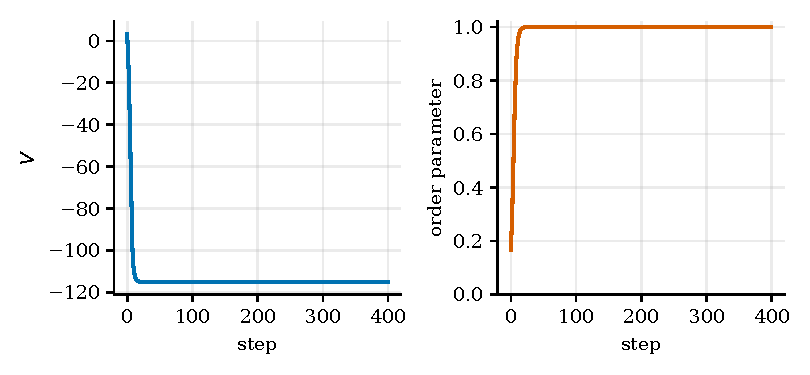
\includegraphics[width=0.85\textwidth]{figs/kuramoto}
\caption{Euler-discretized Kuramoto dynamics with $\omega_i=0$ on a random sparse symmetric coupling of 30 oscillators at step $0.9/\kappa$: the potential $V$ (decreasing at every step, as asserted) and the order parameter. Computed by the script \texttt{figs.py} with seed 8; an illustration of the stated analytic result and not an evaluation of the architecture.}\label{fig:kuramoto}
\end{figure}

\chapter{The Ecphoric Retrieval Engine}\label{ch:engine}

Retrieval is an iterative computation, and the specification must fix its initialization, its candidate activation, its refinement step, its convergence criterion, its confidence estimate, and its termination rule. The iteration is
\begin{equation}\label{eq:engine}
r^{(k+1)}=\mathcal T_\vartheta\bigl(r^{(k)},c,M,Z,\Theta^{(k)}\bigr),
\end{equation}
with the minimal instance $\mathcal T_\vartheta(r)=(1-\eta)r+\eta\sum_iw_im_i$ of Appendix~\ref{app:minimal}. The initial state is $r^{(0)}=c$, the cue projected into the content space, or $r^{(0)}=0$ if the cue is a pure context. Candidate activation computes the scores $s_i^{(k)}=R(m_i,U(z,\theta^{(k)})c)$ for a subset of traces selected by an index, exact in the baseline and approximate when Chapter~\ref{ch:budget} makes a budget binding. The refinement step is \eqref{eq:engine}, and convergence is declared when the residual $\norm{r^{(k+1)}-r^{(k)}}$ falls below a tolerance $\epsilon_{\mathrm{res}}$.

For a map known to be a $\lambda$-contraction, convergence has a certificate. If the residual at step $k$ is $\varrho_k=\norm{r^{(k)}-r^{(k-1)}}$, then Lemma~\ref{lem:banach} applied at the iterate gives the distance to the fixed point as at most $\lambda\varrho_k/(1-\lambda)$. The termination rule can therefore be stated in terms of a certified distance and not only in terms of a residual: stop when $\lambda\varrho_k/(1-\lambda)\le\epsilon$. For the damped softmax step with $\eta\in(0,1]$ and $\beta<1$, Theorem~\ref{thm:contract} gives the contraction factor $\lambda=1-\eta+\eta\beta$. The certificate is valid only for the fixed point it certifies, and by Example~\ref{ex:constant} it says nothing about whether that fixed point is the historically correct reconstruction.

Confidence estimation is therefore reported on two axes that must not be merged. The first is convergence confidence, the certified distance above. The second is selectivity, the information in the retrieval weights, which can be summarized by the entropy $H(w)$ or by the margin $\Delta=s_{(1)}-s_{(2)}$ between the largest and second largest scores. A sharp margin supports the claim that the output is close to one stored trace, by Proposition~\ref{prop:basin}. Neither axis measures fidelity, which requires the evidence-based statistics of Chapter~\ref{ch:reconsol}, and a conforming implementation must report the first two as properties of the computation and the third only when supporting evidence is available.

\section*{Executable specification of retrieval}\label{sec:retrievecode}

The retrieval engine of this chapter is specified by an iteration, and the lifecycle example at the end of Part~VIII uses its single-step form, so the form that is used is fixed here in pseudocode. The listing is a specification in the sense of Chapter~\ref{ch:refimpl}: it defines the interface and the invariants, it is deterministic given its inputs, and it is not a claim about performance.

\begin{figure}[t]
\centering
\begin{Verbatim}[fontsize=\footnotesize,frame=single,framesep=2mm]
RETRIEVE(M, L, c; beta, g, theta_d, tau)
  # M: traces m_1..m_P with ledger pointers nu_1..nu_P;  L: ledger;  c: cue
  1  for i in 1..P:  cos_i <- <m_i, c> / (|m_i| |c|)
  2  w <- softmax(beta * cos)
  3  F <- sum_i w_i m_i
  4  r <- (1 - g) F + g c                       # one cue-anchored step
  5  margin <- (largest cos) - (second largest cos)
  6  A <- { i : w_i >= tau }                    # attributed traces
  7  D <- { j : r_j >= theta_d }                # reportable details
  8  W <- { j in D : exists i in A with (m_i)_j >= 1/2 }   # warranted details
  9  omega <- |W| / |D|    (omega <- 1 if D is empty)
 10  append to L: interpretation(cue = c, cites = nu_i for i in A,
                                 weights = w, details = D)
 11  return (r, w, A, D, W, omega, margin)      # M is not modified
\end{Verbatim}
\caption{Single-step retrieval with attribution and warrant coverage. The traces are never modified by retrieval, and the only persistent effect is the appended interpretation record. The parameters used in the lifecycle example are $\beta=8$, $g=0.2$, $\theta_d=\tfrac14$ and $\tau=\tfrac12$.}\label{fig:retrievecode}
\end{figure}

Three properties of the listing are used below. Retrieval is a read-only operation on the store, so the persistent state after a retrieval differs from the state before it only by one ledger record. The warrant coverage $\omega$ of line 9 is computed from the stored traces and the attributed set $A$ and not from the reconstruction, so it can be low when the reconstruction is dominated by the cue; this is the separation between generative influence and warrant of Definition~\ref{def:warrant}. And the set $A$ may be empty, in which case $W$ is empty and $\omega=0$ for a nonempty $D$, which is how the specification reports that no single stored trace accounts for the answer.


\chapter{Persistent Memory and Historical Provenance}\label{ch:provenance}

The architecture must permit modification of a memory without silently rewriting the record of what was previously stored. The mechanism is an append-only ledger. A ledger is a set of typed records, each carrying an identifier, a type, a payload, a reference to the records it depends on, and a logical timestamp. Four record types are distinguished. An inscription records the original encoding of an observation: the content as first written, with the context and time. A transformation records a subsequent change to a trace, with the exact increment of Proposition~\ref{prop:reverse}. An interpretation records a reconstruction produced by the retrieval engine together with the cue and context that produced it, so that reconstructions are never confused with inscriptions. An evidence record records an observation that supports or contradicts a prior record and is the stated reason for any transformation that cites it. The pointer $\nu_i$ of a trace is the identifier of its latest record, and the full chain of records reachable from $\nu_i$ is the provenance of the trace.

A distinction that the ledger must support is between the evidence that generated a reconstruction and the evidence that warrants its historical attribution. A reconstruction can be causally influenced by a trace without that trace justifying every detail of the result: the weight a trace receives in the retrieval iteration measures its contribution to the computation, and says nothing about whether the inscription behind it entails a particular detail of the output, which may have been supplied by the context operator, by the cue, or by the blending of several traces. The two relations are recorded separately.

\begin{definition}[Generative influence and warrant]\label{def:warrant}
Let an interpretation record carry a reconstruction $r^\star$ with a set $A$ of separately reportable details. Its generative influence is the weight vector $w^{(K)}$ of the final refinement step, together with the sources of the cue and the context used. A detail $a\in A$ is warranted if there is an attributed trace, that is, a trace whose weight in $w^{(K)}$ is at least a declared attribution threshold $\tau_{\mathrm{attr}}$ (by default $\tfrac12$), such that the inscription record at the head of its citation chain, together with the logged transformations on that chain, determines the value of $a$ to within the stated tolerance under a declared entailment rule. The warrant coverage of the record is $\omega=|\{a\in A:a\text{ is warranted}\}|/|A|$, and the details outside the warranted set are labeled inferred.
\end{definition}

Warrant coverage is computed from the ledger and the entailment rule, independently of the retrieval weights, so a reconstruction with high generative influence from a trace and low warrant coverage is detected as one whose details were largely supplied by something other than the record. Source attribution in the sense of Chapter~\ref{ch:source} is a claim about warrant and not about influence, and the experiments of Chapter~\ref{ch:source-exp} measure it as such.

Three properties follow from the append-only discipline. The first is auditability: the chain from any trace to its inscription is available, and every transformation can be traced to its evidence. The second is reversibility, shown for logged increments in Proposition~\ref{prop:reverse}: any earlier state of a trace is recoverable from the current state and the ledger. The third is non-forgery: since interpretations are typed distinctly from inscriptions, a reconstruction cannot be mistaken for the original even if it is later promoted to a stored trace, because the promotion is itself a recorded transformation citing the interpretation as its source. This last property is what separates a system that has revised its memory from one that has lost track of its own history.

Deliberate forgetting is accommodated without breaking append-only semantics by tombstones. A tombstone is a record of type release that references the records it supersedes. Under the default policy of Chapter~\ref{ch:forgetting} the payloads of the superseded records are retained in cold storage so that the release is reversible; under an erasure policy the payloads are deleted and the tombstone records the fact and the time of deletion. In either case the ledger records that the release occurred, and what is lost under erasure is the content, never the knowledge that the content once existed. The relation between the ledger and the sufficiency criterion is direct: by the first qualification after Proposition~\ref{prop:identlimit}, a decoder that consults the ledger has the ledger as part of the memory state, and the sufficiency question is then asked of the combined encoding. This is the formal reason that source discrimination, which is impossible from content alone (Proposition~\ref{prop:source}), becomes possible when provenance is stored.


\begin{figure}[t]
\centering
\begin{tikzpicture}[>=Stealth,rec/.style={draw,rounded corners=2pt,minimum width=3.0cm,minimum height=.9cm,align=center,font=\small}]
\node[rec] (ins) at (0,0) {inscription\\observation $o$};
\node[rec] (tr) at (4.6,0) {transformation\\increment $\Delta_s$};
\node[rec] (rel) at (9.2,0) {release\\tombstone};
\node[rec] (int) at (0,-2.4) {interpretation\\reconstruction $r^\star$};
\node[rec] (ev) at (5.2,-2.4) {evidence\\supports or contradicts};
\draw[->] (tr) -- node[above,font=\scriptsize] {cites} (ins);
\draw[->] (rel) -- node[above,font=\scriptsize] {cites} (tr);
\draw[->] (ev) -- node[right,font=\scriptsize] {gates} (tr);
\draw[->] (int) -- node[left,font=\scriptsize] {cites} (ins);
\draw[->,dashed] (int) -- node[below,font=\scriptsize] {promoted} (ev);
\end{tikzpicture}
\caption{Typed records of the ledger and their citation structure. Arrows point from a record to the records it depends on; no record is removed, and a reconstruction can enter the store only through a transformation that cites it.}\label{fig:ledger}
\end{figure}

\section*{Executable specification of ledger replay}\label{sec:replaycode}

The derived state of Proposition~\ref{prop:derived} is computed by a fold, and the fold is the object that the replay requirement of the reference implementation tests.

\begin{figure}[t]
\centering
\begin{Verbatim}[fontsize=\footnotesize,frame=single,framesep=2mm]
REPLAY(L, init)
  # L: ledger records with Lamport timestamps;  init: payload -> initial vector
  1  M <- []                                  # list of traces, indexed by inscription
  2  for rec in L sorted by (counter, replica_id):
  3     if rec.type == inscription:
  4         append copy(init[rec.payload]) to M;  index[rec.id] <- len(M)
  5     if rec.type == transformation:
  6         i <- index of the trace cited first by rec
  7         M[i] <- M[i] + rec.payload          # logged increment, exact
  8     if rec.type == release:
  9         mark the trace cited by rec as released (payload kept in cold storage)
 10     # interpretation and evidence records do not change M
 11  return M
\end{Verbatim}
\caption{Deterministic derivation of the store from the ledger. The result depends only on the set of records, by Proposition~\ref{prop:derived}.}\label{fig:replaycode}
\end{figure}

A remark on arithmetic is needed, because Proposition~\ref{prop:reverse} is stated in real arithmetic and an implementation uses finite precision. Recovering an earlier state by subtracting later increments from the current state is exact in real arithmetic, but in floating point it can leave a rounding residue, since addition is not associative. The specification therefore recovers an earlier state by replaying the ledger up to the chosen time, and it uses subtraction only as an audit check. In the lifecycle example below all stored values and increments are dyadic rationals of small denominator, for which floating-point addition and subtraction are exact, so that both procedures agree bit for bit, and this is the reason those values were chosen. The choice is a device of the example; it does not make the property hold for arbitrary payloads.

Definition~\ref{def:warrant} counts a detail as warranted only through an attributed trace, and the lifecycle example shows why the threshold is needed. Under a softmax every trace has strictly positive weight, so if warrant required only positive generative influence then every detail present in any stored trace would be warranted and the coverage $\omega$ would be vacuous. The definition therefore requires the weight to reach $\tau_{\mathrm{attr}}$, a declared policy parameter, and takes the content of the trace to be its inscription together with its logged transformations, which is the form used by the listing of Figure~\ref{fig:retrievecode}.


\chapter{Adaptive Memory Organization}\label{ch:adaptive}

Five operations organize the store over time: consolidation, splitting, merging, abstraction, and forgetting. For each the specification must state an invariant for provenance, for accessibility, and for recoverability, and the invariants are the acceptance conditions for any implementation.

Consolidation transfers strength from the fast to the slow store by replay, with the dynamics of Proposition~\ref{prop:twostore}; its provenance invariant is that the slow-store trace carries the pointers of the fast-store traces it was built from, and its accessibility invariant is that the cue family supported before consolidation remains supported with at most the distortion allowed by the replay's learning rate. Splitting replaces a trace by two when a cue family is found to require a distinction that the trace blurs, such as when the same content has been associated with conflicting outcomes in different contexts; the provenance invariant is that both children cite the parent, and the recoverability invariant is that the parent is reconstructible from the pair, which holds exactly when the split is an additive decomposition $\psi=\psi'+\psi''$ and the ledger records the weights. Merging replaces a set of traces by one when they are redundant with respect to the committed cue family. Its admissibility is a corollary of Proposition~\ref{prop:distort}: merging two traces that differ by $\delta$ in norm replaces each by their mean, a displacement of $\delta/2$ per trace, so the readout changes by at most $(1+2\beta)\delta/2$ at every query in the unit ball, and the merge is admissible when this is below the tolerance $\varepsilon$ of the compression bound \eqref{eq:compbound}. Abstraction creates a trace representing a class by the mean of its members, retaining the members in the ledger; it is the operation by which the slow store acquires semantic structure, and its admissibility is the closure criterion of Proposition~\ref{prop:closure} for the projection that sends members to the class. Forgetting follows Chapter~\ref{ch:forgetting} and always leaves a tombstone.

\begin{proposition}[Provenance is preserved by every organizing operation]\label{prop:provinv}
Suppose each of the five operations is implemented as an append of new records that reference the records they act on, and never as a modification or deletion of an existing record, except that erasure policy may delete payloads of released records. Then for every trace present at any time, the chain from its pointer to the inscriptions of the observations it derives from is complete, and the set of records only grows.
\end{proposition}

\begin{proof}
Each operation appends records that cite their inputs, so by induction on the number of operations every trace's chain reaches inscriptions through citations that are never removed. The set of records grows monotonically because no operation removes a record, and erasure removes only payloads, which does not alter the citation structure.
\end{proof}

\section*{Executable specification of controlled reconsolidation and a merge check}\label{sec:reconcode}

The evidence-gated update of Chapter~\ref{ch:reconsol} and the provenance invariant of Proposition~\ref{prop:provinv} fix what a revision must do, and the listing below fixes how.

\begin{figure}[t]
\centering
\begin{Verbatim}[fontsize=\footnotesize,frame=single,framesep=2mm]
RECONSOLIDATE(M, L, i, e, reports; eta, Lambda_star)
  # i: trace to revise;  e: evidence-bearing target;  reports: {(source, rho)}
  1  keep one report per distinct source          # no double counting
  2  Lambda <- product over kept reports of rho / (1 - rho)
  3  ev <- append to L: evidence(cites = nu_i, payload = reports)
  4  if Lambda < Lambda_star:  return M           # gate closed, store unchanged
  5  Delta <- eta * (e - m_i)                      # exact increment
  6  tr <- append to L: transformation(cites = nu_i and ev, payload = Delta)
  7  m_i <- m_i + Delta;  nu_i <- tr
  8  return M

REVERSE(M, L, i, tr)
  1  Delta <- payload of tr
  2  tr' <- append to L: transformation(cites = nu_i and tr, payload = -Delta)
  3  m_i <- m_i - Delta;  nu_i <- tr'              # nothing is deleted
\end{Verbatim}
\caption{Evidence-gated revision and its reversal. The evidence record is appended whether or not the gate opens, so that the rejected evidence remains auditable. Reversal appends an inverse increment and does not remove records.}\label{fig:reconcode}
\end{figure}

By construction every operation in the listing appends and none removes, so the hypothesis of Proposition~\ref{prop:provinv} holds, and by Proposition~\ref{prop:derived} the store after any sequence of operations equals the replay of its ledger. The gate of line 4 aggregates by source, which is the discipline that Counterexample~\ref{cex:gate28} shows to be necessary.

\begin{workedex}[Admissibility of a merge]\label{ex:merge42}
Merging two traces at distance $d$ into their midpoint moves each by $d/2$, so by Proposition~\ref{prop:distort} the readout of any cue changes by at most $(1+2\beta)d/2$. A merge is therefore admissible for a compression budget $\varepsilon$ if $d\le2\varepsilon/(1+2\beta)$. For $\beta=8$ and $\varepsilon=0.05$ the threshold is $d\le\ndmax$, a very small distance, which shows that at selective temperatures only near-identical traces can be merged on the strength of this sufficient condition alone. In 300 random stores with a planted near-duplicate pair, the largest observed ratio of the actual readout change to the bound $(1+2\beta)d/2$ was $\nmergeratio$. The bound was therefore never violated and was loose by a factor of about thirty-seven on those stores. Because Extension~\ref{ext:sharp30} shows that the dependence on $\beta$ cannot be improved in general, a larger threshold must come from structural knowledge of the cue family, which is what the quotient of Extension~\ref{ext:viabequiv} provides. These are algebraic checks of the proposition with a fixed seed and not measurements on a memory.
\end{workedex}


\paragraph{A unified learning objective.} The operations above are mechanisms, and a trainable architecture needs a single objective that couples them. Let $\vartheta$ collect the continuous parameters of the representation (the encoder of content and the context operator $U$), of the oscillatory engine ($\omega$, $K$), and of the retrieval engine ($\beta$, $\eta$, any gating maps), and let the discrete operations (merging, splitting, release) be governed by rules whose thresholds are hyperparameters. Over streams of episodes and cues with targets $T$, the learning problem is
\begin{equation}\label{eq:learnobj}
\min_{\vartheta}\ \Ex\Bigl[\sum_t\ell\bigl(r^\star_t(\vartheta),T(h_t,c_t)\bigr)+\lambda\,C_t(\vartheta)\Bigr]\quad\text{subject to}\quad\Ex[D_t]\le\delta\ \text{and}\ X_t\in\Viab(K)\ \ \text{for all }t,
\end{equation}
where $\ell$ is the reconstruction loss, $C_t$ the computational cost, $D_t$ the fidelity distortion of Chapter~\ref{ch:viability}, and the second constraint confines the discrete operations to the viability kernel. The constraints are handled by a Lagrangian with a multiplier on the fidelity term updated by dual ascent, which converges to a solution that respects the constraint and, unlike a fixed penalty, does not depend on the scale of the loss (Proposition~\ref{prop:penalty}). The retrieval engine is differentiable in $\vartheta$ whenever it is a contraction, which makes the objective trainable without backpropagating through the unrolled iteration.

\begin{proposition}[Implicit differentiation through a contractive retrieval]\label{prop:implicit}
Let $F(r;\vartheta)$ be continuously differentiable jointly in $(r,\vartheta)$ with $\norm{\partial_rF}\le\lambda<1$ and $\norm{\partial_\vartheta F}\le L_\vartheta$. Then the fixed point $r^\star(\vartheta)$ is continuously differentiable and
\begin{equation}
\frac{\partial r^\star}{\partial\vartheta}=\bigl(I-\partial_rF\bigr)^{-1}\partial_\vartheta F\Big|_{r^\star},\qquad\Bigl\|\frac{\partial r^\star}{\partial\vartheta}\Bigr\|\le\frac{L_\vartheta}{1-\lambda}.
\end{equation}
\end{proposition}

\begin{proof}
Since $\norm{\partial_rF}<1$, the matrix $I-\partial_rF$ is invertible with $\norm{(I-\partial_rF)^{-1}}\le1/(1-\lambda)$ by the Neumann series. The implicit function theorem applied to $r-F(r;\vartheta)=0$ gives differentiability and the formula, and the bound follows.
\end{proof}

The learning problem \eqref{eq:learnobj} makes the relation among consolidation, reconsolidation and the representation explicit: they are components of one constrained optimization, in which consolidation shapes the targets that the loss measures, evidence-gated reconsolidation changes the targets $T$ only through recorded evidence, and the representation and oscillator parameters are learned against the resulting stream. The specification does not claim that the optimization has been carried out; it states what the training problem is, so that the experiments of Part~IX have a defined object to train.

\chapter{Resource Scheduling and Bounded Computation}\label{ch:budget}

The ideal system of Part~VII has no resource limits, and the practical system has a budget $B_t$ on time, memory and energy. The scheduler decides, for each retrieval, how many refinement steps to spend, how many traces to activate, and whether to attempt reconstruction at all. The central quantity is the marginal value of a further step, which for a contractive refinement can be stated exactly.

Suppose the iteration is a $\lambda$-contraction with initial certified error $R$ and that each step costs $\varsigma>0$ in the units of the objective, with the penalty for remaining error equal to the error itself. The total cost after $k$ steps is bounded by
\begin{equation}\label{eq:budgetcost}
J(k)=R\lambda^k+\varsigma k,
\end{equation}
where the first term is the error bound of Lemma~\ref{lem:banach}.

\begin{proposition}[Optimal stopping for contractive refinement]\label{prop:stopping}
The function $J$ is convex in $k$ and its continuous minimizer is
\begin{equation}
k^\star=\frac{1}{\ln(1/\lambda)}\ln\!\Bigl(\frac{R\ln(1/\lambda)}{\varsigma}\Bigr)
\end{equation}
when $R\ln(1/\lambda)>\varsigma$, and $J$ is minimized at $k=0$ otherwise. The integer minimizer is $\lfloor k^\star\rfloor$ or $\lceil k^\star\rceil$.
\end{proposition}

\begin{proof}
$J''(k)=R(\ln\lambda)^2\lambda^k>0$, so $J$ is convex. Setting $J'(k)=-R\ln(1/\lambda)\lambda^k+\varsigma=0$ gives $\lambda^k=\varsigma/(R\ln(1/\lambda))$, hence $k^\star$. If $R\ln(1/\lambda)\le\varsigma$ then $J'(0)\ge0$ and convexity gives the minimum at zero. For a convex function on the integers the minimizer is one of the two integers adjacent to the continuous minimizer.
\end{proof}

The proposition formalizes the rule that further reconstruction is worth its cost until the marginal reduction of the error bound falls to the marginal cost of a step, and it shows that slow contractions (with $\lambda$ near one) justify a number of steps that grows like $1/\ln(1/\lambda)$. It also identifies the failure mode of a fixed iteration count: an easy cue, with a small $R$, wastes steps, and a hard cue is stopped before the bound is useful.

Graceful degradation under a binding budget has a specification. The retrieval engine reduces cost in a fixed order, first by shortening the refinement, then by restricting activation to the top-$K$ traces by a cheap prefilter, then by lowering the precision of the scores, and only then by declining to answer. At every stage the response reports the residual certificate and the margin of Chapter~\ref{ch:engine}, so that the downstream consumer can tell a reduced-effort answer from a full-effort one. Critical historical distinctions are protected by marking traces whose release or merge would leave the viability kernel of Chapter~\ref{ch:viability}; the scheduler never prefilters them out and never merges them, whatever the budget, which makes this a hard constraint and not a penalty.

Figure~\ref{fig:stopping} shows the trade-off of Proposition~\ref{prop:stopping}: the error bound falls geometrically while cost grows linearly, and the optimum sits where their slopes cancel.

\begin{figure}[t]
\centering
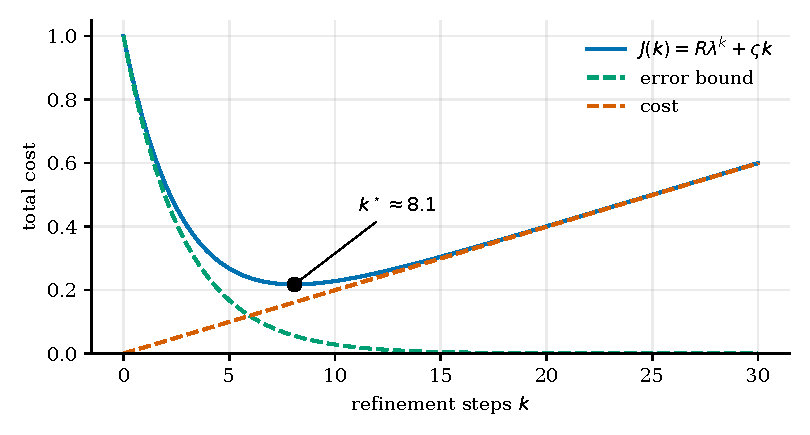
\includegraphics[width=0.85\textwidth]{figs/stopping}
\caption{Total cost $J(k)=R\lambda^k+\varsigma k$ with $R=1$, $\lambda=0.7$, $\varsigma=0.02$, and its minimizer from Proposition~\ref{prop:stopping}. Computed by the script \texttt{figs.py} with seed 8; an illustration of the stated analytic result and not an evaluation of the architecture.}\label{fig:stopping}
\end{figure}

\begin{workedex}[Easy and hard cues under a fixed iteration count]\label{ex:stop43}
Take $\lambda=0.7$ and a step cost $\varsigma=0.02$. For the certified initial error $R=1$ the optimal stopping index is $k^\ast=\nkstar$, the integer optimum is $k=\nkint$ with cost $J(8)=\nJint$, and doing nothing costs $J(0)=\nJA$ while a fixed count of twenty steps costs $J(20)=\nJCA$, nearly twice the optimum. For an easy cue with $R=0.05$ one has $R\ln(1/\lambda)=0.018<\varsigma$, so Proposition~\ref{prop:stopping} says to take no step, at cost $\neasyJA$, and a fixed count of eight would cost $\neasyfixed$, which is $\neasyratio$ times as much. For a hard cue with $R=5$ the optimum is $k^\ast=\nhardk$, the integer minimizer is $\nhardkint$ with cost $\nhardJopt$, and stopping at the fixed count of eight costs $\nhardfixed$, a factor $\nhardratio$ above the optimum. The same fixed count is thus too long for one cue and too short for the other, which is the failure mode that the certified residual is meant to remove. These costs are computed from the formula $J(k)=R\lambda^k+\varsigma k$ and do not describe a measured system.
\end{workedex}


\chapter{Distributed and Asynchronous Memory}\label{ch:distributed}

Several nodes may hold replicas of a memory and update them concurrently, with delayed observations and temporarily inconsistent local histories. The architecture requires eventual reconciliation without loss of any node's inscriptions. The ledger of Chapter~\ref{ch:provenance} provides the natural structure, since a set of records with set union as the merge operation has the algebra needed.

\begin{proposition}[Convergence of ledger replicas]\label{prop:crdt}
Let each replica hold a set of records, grow it by adding records, and merge by set union. Then merge is commutative, associative and idempotent, so any two replicas that have received the same set of records, in any order and with any duplication, hold the same set. Equivalently, the replica states form a join-semilattice under inclusion, and every replica's state is monotone under updates and merges.
\end{proposition}

\begin{proof}
Union is commutative, associative and idempotent. Two replicas that have received the same collection of records, however ordered and duplicated, hold the union of that collection, which is a single set.
\end{proof}

Agreement on the set of records is not yet agreement on the derived memory state, because transformations may not commute: applying an increment $\Delta_1$ followed by a gated update is different from the reverse. The derived state is therefore defined as a fold of the update function over the records in a canonical total order. Give every record a Lamport timestamp \cite{lamport1978} $(\ell,\mathrm{id})$ consisting of a logical counter and the identifier of the originating replica; the lexicographic order on pairs is total, is consistent with causality, and is the same at every replica.

\begin{proposition}[Deterministic derived state]\label{prop:derived}
If the update function is deterministic and records are folded in the order of their timestamps $(\ell,\mathrm{id})$, then any two replicas holding the same set of records compute the same memory state. Late-arriving records with earlier timestamps are accommodated by replaying from the first affected position.
\end{proposition}

\begin{proof}
The timestamp order is a total order on the common set, so the fold is the same sequence of applications at both replicas, and a deterministic update function yields the same result. A late record changes the sequence only from its own position onward, so replaying from that position reproduces the fold.
\end{proof}

The proposition is the formal basis for the replay requirement of the reference implementation. Its cost is the replay length, and the obvious engineering response is periodic snapshots, which are caches of derived state and not memory state, and are discarded when a late record invalidates them. Where updates commute, as with additive increments, the order is immaterial and replay can be avoided entirely.

The distinction between shared semantic knowledge and independently acquired episodic evidence has a precise form in this setting. Semantic content, the slow-store abstractions of Chapter~\ref{ch:adaptive}, is replicated and reconciled by consolidating the union of the nodes' episodic records, and it is an output of the fold. Episodic evidence is never overwritten by another node's semantic abstraction; it is a record in the ledger with the identifier of the node that observed it. A node that receives a conflicting abstraction can compare it with its own episodic records, which is the mechanism by which inconsistent local histories are detected and not merely overwritten.

\begin{workedex}[Non-commuting updates at two replicas]\label{ex:replica44}
Let the memory state be a single number $s$ with initial value $1$. Replica $A$ produces the record $a=(\ell{=}1,A,\text{scale by }2)$ and replica $B$ the record $b=(\ell{=}1,B,\text{add }3)$ concurrently. If a replica applies records in the order of arrival, the node that receives $a$ first computes $1\cdot2+3=\nrepAB$ and the node that receives $b$ first computes $(1+3)\cdot2=\nrepBA$, so two replicas that hold the same set of records disagree on the state, although Proposition~\ref{prop:crdt} guarantees that they agree on the set. Folding in the Lamport order $(\ell,\mathrm{id})$ places $a$ before $b$ at both replicas and gives $\nrepAB$ at each. Suppose now a record $c=(\ell{=}0,C,\text{add }10)$ from a third replica arrives late. The canonical order is $c,a,b$, and replaying from the first affected position gives $((1+10)\cdot2)+3=\nreplate$ at every replica, whatever order the three records were received in, which is the statement of Proposition~\ref{prop:derived}. Where updates commute, as for additive increments, the arrival order would have sufficed and replay could be skipped, which is the cost saving noted after the proposition.
\end{workedex}


\chapter{Reference Implementation}\label{ch:refimpl}

The reference implementation is organized as six modules whose interfaces are fixed so that each can be replaced independently: the representation (encoding and decoding of the trace tuple), the resonance scorer $R$, the oscillator $\mathfrak C$ of Chapter~\ref{ch:oscengine}, the ecphoric reconstruction engine of Chapter~\ref{ch:engine}, the provenance store of Chapter~\ref{ch:provenance}, and the evaluation harness. Replaceability is not a convenience; it is what makes the ablation experiments of Part~IX meaningful, because an ablation changes exactly one module and holds the others fixed.


\begin{figure}[t]
\centering
\begin{tikzpicture}[>=Stealth,box/.style={draw,rounded corners=2pt,minimum width=3.0cm,minimum height=.95cm,align=center,font=\small}]
\node[box] (cue) at (0,0) {cue $c$\\context $Z$};
\node[box] (osc) at (4.3,0) {oscillator\\$\mathfrak C$};
\node[box] (score) at (8.6,0) {scorer $R$\\weights $w^{(k)}$};
\node[box] (out) at (0,-2.3) {reconstruction $r^\star$\\certificate, margin};
\node[box] (eng) at (4.3,-2.3) {retrieval engine\\$r^{(k+1)}=\mathcal T_\vartheta(\cdot)$};
\node[box] (mem) at (8.6,-2.3) {persistent traces\\$M$};
\node[box] (led) at (4.3,-4.6) {ledger\\(append only)};
\draw[->] (cue) -- (osc);
\draw[->] (osc) -- node[above,font=\scriptsize] {$\Phi^{(k)}$} (score);
\draw[->] (mem) -- (score);
\draw[->] (score.south west) -- (eng.north east);
\draw[->] (eng) -- (out);
\draw[->] (eng) -- node[right,font=\scriptsize] {interpretation record} (led);
\draw[->] (led.east) -| node[below right,font=\scriptsize,pos=.2] {$\nu_i$} (mem.south);
\draw[->,dashed] (eng.north) -- node[left,font=\scriptsize,pos=.4] {$r^{(k)}$} (osc.south);
\end{tikzpicture}
\caption{Module structure of the reference implementation. Each box is an independently replaceable module; the dashed arrow is the feedback of the current reconstruction into the context operator and the scores, absent in the minimal model of Appendix~\ref{app:minimal}.}\label{fig:modules}
\end{figure}

Three engineering requirements are binding. The first is determinism: with fixed seeds and a fixed order of events the implementation must produce bit-identical memory states, so that Proposition~\ref{prop:derived} is realized in code and any discrepancy is a defect. The second is instrumentation: every retrieval emits the cue, the context, the scores, the weights, the iterates, the residual certificates and the final reconstruction to an interpretation record, so that nothing about a reconstruction is discoverable only by rerunning it. The third is replay: any memory transition can be reproduced from the ledger and the seed, and the test suite includes a replay check that rebuilds the state from the ledger and compares it with the live state.

The minimal model of Appendix~\ref{app:minimal} is the first conforming instance. Its deliberately limited scope should be stated: it has no learning rules, no temporal sequence representation, no uncertainty beyond the retrieval weights, and no persistent-state updates, and the modules above are specified so that each of these can be added without changing the others. The pilot calculations of Appendix~\ref{app:pilot} check the algebraic claims of Parts~II and III in this setting and do not constitute an evaluation of the architecture.

\section*{A complete miniature memory lifecycle}\label{sec:lifecycle}

The components of Part~VIII are exercised together by a deterministic walk through one memory from encoding to revision and audit. The setting is deliberately tiny so that every number can be inspected: seven binary features (\emph{Ann}, \emph{Bo}, \emph{cafe}, \emph{library}, \emph{rain}, \emph{morning}, \emph{evening}), three episodes $E_1=(\emph{Ann},\emph{cafe},\emph{morning})$, $E_2=(\emph{Ann},\emph{library},\emph{rain})$ and $E_3=(\emph{Bo},\emph{cafe},\emph{rain})$, and the parameters $\beta=8$, $g=0.2$, $\theta_d=\tfrac14$, $\tau_{\mathrm{attr}}=\tfrac12$ and $\Lambda^\ast=10$. The procedures are those of Figures~\ref{fig:retrievecode}, \ref{fig:replaycode} and~\ref{fig:reconcode}. The script \texttt{lifecycle.py} carries out every step with exact arithmetic and asserts, after every operation, that the ledger has only grown and that replaying it reproduces the store. The walk is an illustration of the specification on invented data and is not an empirical finding.

\begin{table}[p]
\centering
\small
\renewcommand{\arraystretch}{1.2}
\begin{tabular}{@{}l p{3.0cm} p{5.2cm} p{2.6cm}@{}}
\toprule
Step & Operation & Persistent traces after the operation & Ledger records \\
\midrule
S0 & empty store & \footnotesize (empty) & \footnotesize none \tabularnewline
S1 & encode E1 & \footnotesize $m_1=(1,0,1,0,0,1,0)$ & \footnotesize 1i \tabularnewline
S2 & encode E2, E3 & \footnotesize $m_1=(1,0,1,0,0,1,0)$\par $m_2=(1,0,0,1,1,0,0)$\par $m_3=(0,1,1,0,1,0,0)$ & \footnotesize 1i 2i 3i \tabularnewline
S3 & partial cue (Ann, morning) & \footnotesize $m_1=(1,0,1,0,0,1,0)$\par $m_2=(1,0,0,1,1,0,0)$\par $m_3=(0,1,1,0,1,0,0)$ & \footnotesize 1i 2i 3i 4p \tabularnewline
S4 & misleading cue (adds rain) & \footnotesize $m_1=(1,0,1,0,0,1,0)$\par $m_2=(1,0,0,1,1,0,0)$\par $m_3=(0,1,1,0,1,0,0)$ & \footnotesize 1i 2i 3i 4p 5p \tabularnewline
S5 & misleading report, gate closed & \footnotesize $m_1=(1,0,1,0,0,1,0)$\par $m_2=(1,0,0,1,1,0,0)$\par $m_3=(0,1,1,0,1,0,0)$ & \footnotesize 1i 2i 3i 4p 5p 6e \tabularnewline
S6 & corroborated evidence, revise m1 & \footnotesize $m_1=(1,0,1,0,0,0,1)$\par $m_2=(1,0,0,1,1,0,0)$\par $m_3=(0,1,1,0,1,0,0)$ & \footnotesize 1i 2i 3i 4p 5p 6e 7e 8t \tabularnewline
S7 & later recollection (Ann, evening) & \footnotesize $m_1=(1,0,1,0,0,0,1)$\par $m_2=(1,0,0,1,1,0,0)$\par $m_3=(0,1,1,0,1,0,0)$ & \footnotesize 1i 2i 3i 4p 5p 6e 7e 8t 9p \tabularnewline
S8 & replay from ledger (state identical) & \footnotesize $m_1=(1,0,1,0,0,0,1)$\par $m_2=(1,0,0,1,1,0,0)$\par $m_3=(0,1,1,0,1,0,0)$ & \footnotesize 1i 2i 3i 4p 5p 6e 7e 8t 9p \tabularnewline
S9 & audit: rewind 8t, read only (store unchanged) & \footnotesize $m_1=(1,0,1,0,0,0,1)$\par $m_2=(1,0,0,1,1,0,0)$\par $m_3=(0,1,1,0,1,0,0)$ & \footnotesize 1i 2i 3i 4p 5p 6e 7e 8t 9p \tabularnewline
S10 & reverse revision: append inverse transformation & \footnotesize $m_1=(1,0,1,0,0,1,0)$\par $m_2=(1,0,0,1,1,0,0)$\par $m_3=(0,1,1,0,1,0,0)$ & \footnotesize 1i 2i 3i 4p 5p 6e 7e 8t 9p 10t \tabularnewline
\bottomrule

\end{tabular}
\caption{The persistent state after every operation of the lifecycle. Ledger records are numbered in order of creation and suffixed by type: i inscription, p interpretation, e evidence, t transformation. Retrieval steps change only the ledger, and the only steps that change a trace are S6 and S10.}\label{tab:lifecycle}
\end{table}

\paragraph{Encoding and partial-cue reconstruction (S1 to S3).} Encoding the three episodes appends three inscriptions and creates three traces. The cue $(\emph{Ann},\emph{morning})$ is partial, since it does not mention the place. Retrieval gives weight $\nwA$ to the first trace and $\nwAtwo$ to the second, with a cosine margin of $\nmarginA$ between the best and the second best trace, so the first trace is the single attributed trace. The reconstruction contains the details \emph{Ann}, \emph{cafe} and \emph{morning}; the cafe is supplied by the stored trace and not by the cue, and it is warranted by that trace, so the warrant coverage is $\nomegaA$. The store is unchanged and the ledger gains an interpretation record, 4p.

\paragraph{Misleading cue (S4).} The cue $(\emph{Ann},\emph{cafe},\emph{morning},\emph{rain})$ adds a feature that episode $E_1$ does not contain. The first trace still receives weight $\nwB$ and is attributed, but the reconstruction now reports \emph{rain} among its details, with component $\nrainB$ in the reconstructed vector, supplied by the cue and by the other traces and not by the attributed one. Warrant coverage is $\nomegaB$, three of the four details, and the report labels \emph{rain} as inferred. The example also shows the danger that Proposition~\ref{prop:drift} describes. If the reconstruction were written back to the first trace with rate $\tfrac12$ and no evidence, the trace would move by $\nhypshift$ in norm and acquire a rain component of $\nhyprain$ that no observation supports. The specification does not do this; the store is unchanged and the ledger gains 5p.

\paragraph{Misleading and then corroborating evidence (S5 and S6).} A single report that the episode took place at the library, from a source of reliability $0.6$, has likelihood ratio $\nlamone$ and the gate stays closed at $\Lambda^\ast=10$. The evidence is nonetheless recorded (6e), so the rejected report remains auditable. Three reports from three distinct sources, each of reliability $0.7$ and each saying that the episode was in the evening, give $\Lambda=\nlamthree$ and the gate opens. The revision moves the first trace by the increment $\Delta=e-m_1$ with $e=(\emph{Ann},\emph{cafe},\emph{evening})$, which flips the morning and evening features and moves the trace by $\nLdist$ in norm. The ledger gains the evidence record 7e and the transformation 8t, which cites the inscription 1i and the evidence 7e. The one-vote-per-source rule of Figure~\ref{fig:reconcode} matters here, since three copies of one report would have given only $\Lambda=\nlamcopy$ (Counterexample~\ref{cex:gate28}).

\paragraph{Later recollection (S7).} The cue $(\emph{Ann},\emph{evening})$ now attributes weight $\nwC$ to the revised trace and returns warrant coverage $\nomegaC$ with an interpretation record that cites the transformation 8t. The revision also changes how the original cue behaves: the cue $(\emph{Ann},\emph{morning})$, which gave weight $\nwA$ before the revision, gives only $\nwOldCue$ afterwards, below the attribution threshold, so no single trace is attributed to it and the specification reports that no trace accounts for the answer. This is the intended consequence of a justified revision and not an error.

\paragraph{Replay, audit and reversal (S8 to S10).} Replaying the ledger from the inscriptions reproduces the store exactly (S8). Subtracting the logged increment from the current state recovers the state at S5, so the audit of S9 changes nothing. Reversal (S10) appends an inverse transformation citing 8t, which returns the first trace to its original value while the ledger grows to $\nnledger$ records, none deleted, and a second replay again reproduces the store. The history of the memory therefore contains the revision and its undoing, and both remain open to inspection.

\begin{extension}[Lifecycle invariants]\label{ext:lifecycle}
Let the operations of Figures~\ref{fig:retrievecode}, \ref{fig:replaycode} and~\ref{fig:reconcode}, together with encoding, be applied in any order with the one-vote-per-source rule and exact arithmetic. Then after every operation (i) the record set is a superset of the record set before it, (ii) $\mathrm{REPLAY}(L)=M$, and (iii) a retrieval leaves $M$ unchanged. The first two are Propositions~\ref{prop:provinv} and~\ref{prop:derived} applied to this operation set, and the third is read off line 11 of Figure~\ref{fig:retrievecode}.
\end{extension}

The extension is a restatement and is included because the lifecycle verifies it at every step of one trajectory, which is evidence that the specification is consistent, and no more than that. It says nothing about whether the revisions are correct, since correctness depends on the evidence, and the evidence in the example was constructed.

\section*{Synthesis of Part~VIII}\label{sec:synth8}

The architecture of Part~VIII can be summarized by one rule and the checks that enforce it: nothing that has been written is removed, and every state is a function of the record set. The retrieval listing returns a reconstruction together with the attribution and warrant that justify it, and leaves the store alone (Figure~\ref{fig:retrievecode}). The reconsolidation listing admits a change to a trace only when evidence aggregated over distinct sources passes the gate, and it logs both the evidence and the increment (Figure~\ref{fig:reconcode}). The replay listing derives the store from the record set in a canonical order, which is what makes replicas that hold the same records agree even when their updates do not commute (Worked Example~\ref{ex:replica44}). The lifecycle ties these together: the misleading cue, the single report and the three reports exercise the three failure modes that the earlier parts identified, namely self-reinforcing distortion (Proposition~\ref{prop:drift}), uncorroborated revision, and double counting of evidence (Counterexample~\ref{cex:gate28}).

The links to the earlier parts are as follows. The sufficiency criterion of Part~VII applies to the combined encoding of store and ledger, by the first qualification after Proposition~\ref{prop:identlimit}, so the ledger is what allows a decoder to report that a detail is inferred, that a trace is no longer attributed to a cue, or that a state existed before a revision; none of these answers is available from the store alone. The quotient of Extension~\ref{ext:viabequiv} determines which traces may be merged or released without leaving the viable set, and the merge check of Worked Example~\ref{ex:merge42} is the conservative version of that determination in the absence of structural knowledge. The scheduling of Chapter~\ref{ch:budget} acts on the retrieval of Figure~\ref{fig:retrievecode}, and Worked Example~\ref{ex:stop43} shows that its stopping rule depends on the certified error of the cue and not on a count. The rates and thresholds of Part~VI enter through $\eta$, $\Lambda^\ast$ and $\beta$.

What the part does not establish is performance. The examples are exact computations on invented data chosen to display the logic of the specification, and the experimental protocols of Part~IX remain protocols. The pilot appendix lists the scripts \texttt{examples.py} and \texttt{lifecycle.py} that produced every number in Parts~VI to VIII, so that a reader can rerun them and obtain the same values.

\part{The Experimental Program}

The chapters of this part are protocols. Each states a hypothesis, the construction of the data, the systems compared, the measurements, the controls, and the criteria under which the hypothesis is counted as supported or as refuted. No experimental outcome is reported in this monograph. The algebraic checks of Appendix~\ref{app:pilot} verify identities and bounds of Parts~II and III and are not evaluations of any claim made here. Where a protocol uses a quantity from the literature, it is quoted as reported by its source.

Two rules apply throughout. The first is the matched-baseline rule of Theorem~\ref{thm:matched}: every comparison with a complex-valued system includes a real-valued system of equal information content, because on the sign-phase subfamily the resonance score reduces to a norm-weighted cosine, and any advantage must therefore be located in the norm factor, in the operators and feature map, or in learning. The second is a requirement of pre-specification: the primary metric, the analysis, and the acceptance threshold are fixed before data are generated, and results for which they were chosen after inspection are labeled exploratory.

Sample sizes are determined by the comparison of two proportions. For a binary success outcome with success probabilities $p_0$ and $p_1$ under two independent arms, a two-sided test at level $\alpha$ with power $1-\beta_{\mathrm{p}}$ requires approximately
\begin{equation}\label{eq:samplesize}
n\ \ge\ \frac{(z_{1-\alpha/2}+z_{1-\beta_{\mathrm p}})^2\bigl(p_0(1-p_0)+p_1(1-p_1)\bigr)}{(p_1-p_0)^2}
\end{equation}
queries per arm, and the paired design used when the same queries are posed to both systems reduces this by the correlation between the arms' outcomes. These are planning formulas and the actual effect sizes are unknown until the experiments are run.

\chapter{Reproduction of the Wave-Based Retrieval Paper}\label{ch:repro}

The first experiment reproduces the reported behavior of Listopad's system \cite{listopad2025} before any extension is tried. The paper represents patterns as complex waveforms $\psi(x)=A(x)e^{\iu\phi(x)}$, scores pairs by the resonance score of Chapter~\ref{ch:resonance}, defines the semantic operators NEG, SHIFT+, INT\_UP and INT\_DOWN on a compact vocabulary, and reports distance histograms, a heatmap of pairwise distances, and retrieval latency. The operators are not given formal definitions in the paper; the candidate definitions of Definition~\ref{def:cand-ops} are therefore the object of the reproduction, and the first deliverable is a report of whether the candidates reproduce the qualitative structure the paper describes, namely that cosine distances for the operator outputs concentrate near a common value while resonance distances separate them into blocks, with NEG aligned with the anti-phased opposite and INT\_UP and INT\_DOWN separated by amplitude.

The latency measurements are reproduced under the reported conditions: pattern length $L=1024$, a store of 500{,}000 patterns, a scalar Java backend, twelve threads, and cold cache. The paper reports an average top-one latency of approximately 135 ms with a 95th percentile near 152 ms, and comparable figures for top-ten and top-hundred queries. The reproduction records the same statistics on its own hardware, with the hardware and software configuration reported alongside. Because the paper describes latency as growing linearly with the dataset size while the reported measurement is at one size, the reproduction measures at several store sizes, from $10^3$ to $5\times10^5$, and fits the dependence; linear growth is expected for an exhaustive scan and is a hypothesis to be tested, not an assumption.

The reproduction includes the comparison the original does not make. Against the unmodified real-valued embeddings, the proposal requires matched real-valued representations of equal information capacity. Concretely, for each complex pattern in $\C^n$ the matched baseline uses a real vector in $\R^{2n}$ with the same number of free parameters, and retrieval by the norm-weighted cosine $\rho\,\cos$ and by the plain cosine. By Theorem~\ref{thm:realif} a retrieval operation that is complex-linear is a special case of a real-linear one, so the baseline is at least as expressive. A reproduction that finds the complex system superior to unmodified cosine retrieval and not superior to the matched baseline has localized the effect to the norm factor, the operators, or the feature map, which is itself a result of the program.

\paragraph{Acceptance.} The reproduction succeeds if the qualitative structure of the operator results is recovered under the candidate definitions and the latency is within a stated factor of the reported figure on comparable hardware. It does not succeed or fail on the question of superiority, which belongs to the later experiments.

\chapter{Ecphoric Pattern Completion}\label{ch:completion}

The hypothesis is that Mem8 recovers the correct episode, not merely the nearest stored vector, when the cue is partial, observations are missing, temporal context is corrupted, or competing historical explanations exist. The experiment is designed so that nearest-neighbor retrieval has a determinate failure mode, which the sufficiency theorem identifies: an episode set is constructed in which several episodes share their content and differ in order, context or outcome, so that retrieval by content alone cannot succeed for the target recollection of Definition~\ref{def:suff}.

Episodes are generated from a controlled grammar with $V$ items, episodes of length $\ell$, and a context label drawn from a finite set. Cues are formed by deleting a fraction of the episode, replacing items by distractors, shifting the temporal code, or presenting an ambiguous partial sequence compatible with two or more stored episodes. The target recollection function $T(h,c)$ is specified for each cue type, and the encoding is audited with the sufficiency criterion before any decoder is run: if the criterion fails for the target, the experiment reports the identifiability bound of Proposition~\ref{prop:identlimit} as the ceiling, and a decoder reaching it is credited with optimal performance, while a decoder above it is a bug. Success is measured by the exact-match rate of the reconstructed episode, by the distance of the reconstruction to the target in the realified space, and by the rate at which the returned episode is a stored episode that differs from the target, which separates lure responses from noise. Systems compared are nearest-neighbor retrieval with cosine, with resonance, the softmax reconstruction without context, the softmax reconstruction with context and phase, and the nonoscillatory recurrent baseline. The sample size for a given contrast follows \eqref{eq:samplesize}, and cue types are analyzed separately because the lure and the noise conditions test different mechanisms.

\chapter{Temporal Sequence Reconstruction}\label{ch:sequence}

The hypothesis concerns the recovery of event order, intervals, nested episodes and temporal boundaries, and it is tested for the claim of Chapter~\ref{ch:binding} that a multi-frequency phase code supports exact recovery of lag within the period of the code. For frequencies $\omega_1,\dots,\omega_J$ with integer periods $T_j$, the lag $t$ is decodable modulo $\operatorname{lcm}(T_j)$ by the Chinese remainder theorem when the periods are pairwise coprime, and the experiment verifies the decoding limit and measures how it degrades with phase noise.

The data are sequences of items with specified onset times, nested structures in which one episode contains others, and boundaries marked by context shifts. Tasks include order judgment between two items, interval estimation, retrieval of the item at a given lag from a cue, and segmentation of a continuous stream into episodes. Systems compared are static embeddings with additive positional codes, recurrent networks, the phase-coded memory with a learned and with a fixed code, and a nonoscillatory dynamical baseline with matched state size. The controls of Chapter~\ref{ch:binding} apply: a phase-shuffled variant in which the phase code is permuted across items, which tests whether performance depends on the phase assignment, and a frozen-phase variant in which phases are fixed after encoding, which tests whether dynamics contribute beyond a static code. Because a static positional encoding is itself a phase code, a positive result for the phase-coded memory over the recurrent network is not a result for oscillation until the frozen-phase variant has been compared.

\paragraph{Segmentation as a separate test.} Temporal phase can encode order and interval but does not determine which events form a single remembered episode, so the experiment separates segmentation from sequence retrieval. Every system is run twice, once with oracle episode boundaries supplied by the generator and once with boundaries inferred by the surprise criterion of Chapter~\ref{ch:episodic} (a boundary where the prediction error of the context state exceeds an adaptive threshold). Boundary quality is scored by the F-measure of detected against true boundaries at a stated temporal tolerance. The segmentation cost is the difference in retrieval accuracy between oracle and inferred boundaries, so that a system cannot be credited for sequence retrieval that depended on boundaries it did not infer, nor charged for a segmentation error as if it were a retrieval error.

\chapter{Contextual Interference and Source Attribution}\label{ch:source-exp}

The hypothesis is that systems which store provenance can attribute source and calibrate false recollection, while systems limited to content cannot, as stated in Proposition~\ref{prop:source}. Datasets are constructed in which identical content appears in different contexts and is associated with conflicting historical outcomes. For each item a ground-truth set of sources is recorded. Queries ask for the content, for the source, and for whether the item was previously encountered; the three correspond to retrieval, source discrimination and familiarity.

The measurements are source accuracy, the rate of false recollection (a confident report of an item or source that was not encountered), calibration of reported confidence measured by the expected calibration error and by the reliability diagram, and the sensitivity of each to changes of context between encoding and retrieval, using the encoding-specificity prediction $S=(1+\cos(z-z_0))/2$ of Proposition~\ref{prop:encspec}. The centroid lure of Proposition~\ref{prop:lure} is tested directly: stores are constructed with a cluster of related items and a lure at the cluster mean, and the rate at which the system endorses the lure as previously seen is recorded as a function of the inverse temperature $\beta$ and the number of related items. The systems compared are a content-only softmax memory, the same with context, the same with the ledger of Chapter~\ref{ch:provenance}, and a baseline that stores explicit source labels, which sets the ceiling for source accuracy. The prediction following from the sufficiency theorem is that source accuracy of any system without access to source information is bounded by the identifiability limit, and the experiment treats any exceedance of that bound as evidence of leakage in the dataset or the pipeline.

\paragraph{Warrant coverage.} In addition to source accuracy, the experiment records the warrant coverage $\omega$ of Definition~\ref{def:warrant} for each reconstruction, and the accuracy of reported confidence separately for warranted and inferred details. A system whose details are mostly inferred but reported with the confidence of warranted ones is miscalibrated in a way that source accuracy on the final answer alone does not reveal.

\chapter{Consolidation and Reconsolidation}\label{ch:reconsol-exp}

The hypothesis is that evidence-gated updating allows adaptation to new evidence while keeping the original record recoverable and resisting unwarranted revision, as argued in Chapter~\ref{ch:reconsol}. Streams of episodes are generated with a latent state that changes at known times, so that earlier interpretations become obsolete. Three types of events are interleaved: confirming evidence, contradicting evidence of controlled strength, and reconstructions retrieved by the system itself and fed back as cues without external evidence.

Two quantities are measured and reported together. Adaptability is the speed with which the system's reconstruction follows a change in the world after contradicting evidence, measured by the number of events to reach a stated accuracy on the new state. Resistance to unwarranted revision is the distortion of stored traces after a sequence of self-generated retrievals with no external evidence, measured as the distance from the original inscription; by Proposition~\ref{prop:drift}, an update rule driven by the system's own output collapses traces toward the reconstruction, and the experiment tests whether the evidence gate prevents it. The recoverability of the original record is tested by reversal: the earlier state is reconstructed from the current state and the ledger, and compared bitwise with the earlier state (Proposition~\ref{prop:reverse}). The systems compared are ungated self-referential updating, evidence-gated updating, and a baseline that never updates, which sets the floor for adaptability and the ceiling for resistance. The result of interest is the trade-off curve between adaptability and resistance as the gate threshold varies, and the claim of the monograph is that the gated system dominates the ungated one on the resistance axis at matched adaptability.

\chapter{Oscillatory Ablation Experiments}\label{ch:ablation}

This is the decisive experiment for the necessity of oscillatory coordination. The question, as posed in the proposal, is whether coordinated oscillatory dynamics improve reconstruction under matched parameter counts, computational budgets and information content. The experiment is designed so that a negative answer is as informative as a positive one.

The full system is compared against five variants that differ from it in exactly one module of Chapter~\ref{ch:oscengine}. The phase-frozen variant fixes phases at their initial values. The phase-randomized variant draws phases from the same marginal distribution independently of state. The frequency-uncoupled variant sets $K=0$ so that each oscillator runs at its own frequency. The nonoscillatory recurrent variant replaces the Kuramoto dynamics by a learned map with the same parameter count and no sinusoidal structure. The static resonance variant removes the contextual operator altogether, so that scoring uses the content alone. Tasks are those of Chapters~\ref{ch:completion} to~\ref{ch:source-exp}, which cover completion, temporal order and source attribution, and the primary outcome is reconstruction accuracy on the target recollection function under each task's cue family.

Matching is the delicate part and is specified in advance. Parameter counts are matched by adjusting the hidden width of the nonoscillatory variant. Computational budget is matched by the number of floating-point operations per retrieval, counted analytically. Information content is matched by holding the encoding $E$ fixed across variants, so that Theorem~\ref{thm:suff} gives the same ceiling to all of them and differences are attributable to the decoder. The analysis uses paired comparisons across a common set of queries with a mixed-effects model for task and seed, and the acceptance rule is stated before the run: oscillation is judged to contribute if the full system exceeds every one of the five variants by at least a pre-specified margin on at least a pre-specified number of tasks, with the seeds as the unit of replication. A result in which the nonoscillatory recurrent variant matches the full system is reported as showing that the oscillatory realization of the computation is not necessary for it, which is consistent with the position of Chapter~\ref{ch:equivalence} that the necessary properties are those of the computation and not its physical substrate.

\paragraph{An integrated longitudinal benchmark.} The component experiments leave open whether the architecture preserves reconstructive capacity over time or merely contains several independently functional subsystems, so the program includes one benchmark that requires the capacities together. A system encounters partially overlapping episodes, later receives misleading information about one of them, undergoes consolidation and compression, and is then asked to reconstruct a particular episode from an incomplete cue. It must recover temporal order, identify the correct historical source, distinguish original evidence from subsequent interpretation, and report uncertainty. The cycle of misleading information, update, compression and query is repeated, and every metric above is reported as a function of the number of cycles, so that the object of study is the trajectory of performance and not a single retrieval. The central comparison is against a system that has the same provenance ledger, the same recurrent inference mechanism, the same storage budget, and the same training data, and differs only in lacking the oscillatory coordination. Without that control, an improvement could be attributed to additional information or engineering capacity and not to the proposed mechanism. The prediction following from Theorem~\ref{thm:dynsuff} is that trace-only systems lose answerability irreversibly at the first compression that crosses the commitment of Corollary~\ref{cor:commit}, while ledger-backed systems recover it at the cost of replay, and the benchmark measures that cost.

\chapter{Scaling and Computational Efficiency}\label{ch:scaling}

The hypothesis is that retrieval cost and accuracy scale as predicted by the capacity analysis of Chapter~\ref{ch:capacity}. Measured quantities are capacity (the number of stored traces at which accuracy falls below a threshold), retrieval latency, throughput in queries per second, update cost per write, energy where it can be measured, and accuracy as the number of related traces grows. The predictions to be tested are specific: the expected number of false activations of Proposition~\ref{prop:falseact} as a function of the threshold, the dimension and the store size, and the exponential capacity of Theorem~\ref{thm:capacity} with its required scaling of $\beta$ with the dimension. The random-pattern model is the best case, so the experiment is repeated on structured stores with clustered traces, where overlaps are larger and the capacity predicted by the margin condition is correspondingly smaller.

Both exact and approximate retrieval are measured. Exact retrieval is the exhaustive scan, with latency linear in the store size at fixed dimension. Approximate retrieval uses an index to restrict activation to a candidate set, and the experiment reports the recall of the true top candidate as a function of the candidate size, because an approximate method that discards the correct trace before refinement cannot be rescued by the refinement. Implementations are compared on CPU and GPU, with memory-mapped storage for stores larger than memory, and latency is reported with percentiles and under cold and warm cache separately. Interference is varied by adding competitor traces and measuring the decline of the target weight against the dilution formula of Proposition~\ref{prop:dilution}. Efficiency claims are reported with the hardware and with the cost of the baseline, since the comparison of latency across implementations on different hardware is not informative.

\chapter{Robustness and Failure Analysis}\label{ch:failure}

The program requires explicit reporting of failure. Successful resonance in a favorable condition is not evidence of general mnemonic competence, and the experiment is organized around the conditions under which the system is expected to fail, so that the failures are located and characterized.

Seven conditions are examined. Catastrophic interference is tested by the sequential learning of tasks with and without replay, measuring the accuracy on earlier tasks. False attractors are mapped by counting fixed points of the retrieval iteration that are not within a stated distance of any stored trace, as a function of $\beta$, $P$ and the overlap structure, against the stability criterion of Theorem~\ref{thm:contract}. Unstable synchronization is examined by driving the oscillator toward global synchrony and measuring the loss of selectivity. Phase noise is added at increasing levels to the phase code, and the degradation is compared with the analytic dependence of the score on phase mismatch. Adversarial cues are constructed by optimizing a perturbation of bounded norm to maximize the weight of a chosen wrong trace; since the weights depend on scores through the Lipschitz map of Proposition~\ref{prop:distort}, the bound gives the minimum perturbation needed to cross a margin, and the experiment measures how far the empirical attack is from that bound. Provenance corruption is tested by removing or altering ledger records and measuring the system's ability to detect the inconsistency, through the check that a replay reproduces the live state. Overconfident reconstruction is measured as the gap between reported confidence and accuracy on cues for which the target is not recoverable by Theorem~\ref{thm:suff}; a system that reports high confidence there is miscalibrated with respect to its own encoding. Each failure is reported with the conditions, the frequency, and the proposed mechanism, and unexplained failures are listed as such.

\part{Interpretation and Limits}

\chapter{What the Architecture Explains}\label{ch:explains}

A monograph that mixes theorems, simulations, neuroscientific motivation and conjecture invites the reader to assign to the whole the confidence that belongs only to the strongest part. This chapter prevents that by sorting the claims of the preceding parts into four classes. A claim is formally demonstrated if it is proved here from stated assumptions. It is simulation-supported if a computation, with stated protocol and outcome, bears on it. It is a neuroscientifically motivated hypothesis if it is suggested by empirical findings but not established by them. It is speculative if it extrapolates beyond all of these.

The formally demonstrated results are those of Parts~II, IV, V, VI and VII, and they are results about the idealized system. They include the closed form $S=\tfrac\rho2(1+\rho c)$ of the resonance score and its invariances (Theorem~\ref{thm:closed}), the equivalence of the complex and real parametrizations (Theorem~\ref{thm:realif}) and the matched-baseline principle that follows (Theorem~\ref{thm:matched}), the ecphoric sufficiency criterion and its minimal-memory corollary (Theorem~\ref{thm:suff}, Corollary~\ref{cor:minimal}), the identifiability limit (Proposition~\ref{prop:identlimit}), the Banach bounds and the contraction and stability criterion of the softmax update (Lemma~\ref{lem:banach}, Theorem~\ref{thm:contract}), the false-activation and capacity bounds under the random-pattern model (Proposition~\ref{prop:falseact}, Theorem~\ref{thm:capacity}), the dilution and centroid-lure results, the drift of self-referential updating (Proposition~\ref{prop:drift}), the failure of penalties to guarantee fidelity (Proposition~\ref{prop:penalty}), and the closure criteria for abstraction. These are conditional on their hypotheses, and the hypotheses are often the substantive content: that traces are random on the sphere, that the dynamics is a contraction, that the target is fixed.

The simulation-supported class is nearly empty by design. The only computations performed in this work are the algebraic checks of Appendix~\ref{app:pilot}, which confirm identities and bounds numerically, and they support no claim about the performance of the architecture. The experimental program of Part~IX is the means by which this class would be populated.

The neuroscientifically motivated hypotheses are three. The first is that the macroscale oscillatory modes reported by Cabral and colleagues \cite{cabral2023} indicate that slow, spatially organized, standing-wave-like dynamics are a feature of the resting rodent brain that could in principle coordinate distributed activity. The study is an imaging study of anesthetized rats, its modes are damped and noise-driven in the authors' own model, and its authors state that the neural and vascular contributions are not separated; it does not address episodic recall, and it is used here as motivation only. The second is that retrieval in biological systems is reconstructive and cue-dependent in the manner of encoding specificity \cite{tulving1973}. The third is that phase relations may carry contextual information, for which the literature cited in Chapter~\ref{ch:binding} is suggestive.

The speculative class contains the proposal that a ledger-based, evidence-gated architecture of the kind specified here would show better calibrated memory modification than ungated ones in realistic settings, that the posterior geometry of Chapter~\ref{ch:geometry} characterizes accessibility, and that any of this bears on biological memory. None is supported beyond the formal results that bound them. Table~\ref{tab:status} lists the principal claims with their class.

\begin{table}[t]
\centering
\small
\renewcommand{\arraystretch}{1.2}
\begin{tabularx}{\textwidth}{@{}>{\raggedright\arraybackslash}X>{\raggedright\arraybackslash}p{3.6cm}@{}}
\toprule
Claim & Status\\
\midrule
Closed form and invariances of the resonance score & Demonstrated\\
Sign-phase reduction to a norm-weighted cosine; matched-baseline principle & Demonstrated\\
Sufficiency criterion; minimal memory; identifiability limit & Demonstrated\\
Contraction and local stability of the softmax update & Demonstrated\\
Exponential capacity under a random-pattern model & Demonstrated, model-conditional\\
Evidence-gated updating resists self-generated drift & Mechanism demonstrated; effect size untested\\
Complex-valued retrieval outperforms matched real baselines & Untested\\
Oscillatory coordination improves reconstruction & Untested\\
Cabral modes as a substrate for episodic recall & Hypothesis, not supported by the cited study\\
Posterior geometry characterizes accessibility & Open problem\\
\bottomrule
\end{tabularx}
\caption{Status of the principal claims of the monograph.}\label{tab:status}
\end{table}

\chapter{Biological Plausibility and Computational Equivalence}\label{ch:equivalence}

The question is which properties of biological oscillations are necessary for the computation that Mem8 specifies, and which are properties of one implementation. The formal results give a partial answer, because they show which computational properties are needed and are silent on the physical ones.

What the theory requires is the following. The encoding must preserve the recollective class of the history for the committed cue family (Theorem~\ref{thm:suff}). Retrieval must select among stored candidates with a margin sufficient for the number of candidates (Proposition~\ref{prop:basin}, Theorem~\ref{thm:capacity}). The cue must be transformable by context so that the same content can be retrieved differently under different contexts (Chapter~\ref{ch:context}). The refinement must be stable, which is a contraction condition with a certificate (Theorem~\ref{thm:contract}). Provenance must be separable from content if source is to be recoverable (Proposition~\ref{prop:source}). None of these requires oscillation. A context operator can be implemented by a phase rotation controlled by an oscillator, by a learned linear map, by a gating network, or by a lookup, and by the matched-baseline principle the oscillatory form is a special case of real-linear transformation with a particular parametrization. Whether the oscillatory parametrization has advantages in sample efficiency, in robustness, or in interpretability is an empirical question that the ablation of Chapter~\ref{ch:ablation} addresses.

Biological systems, if they implement something of this kind, must also meet constraints that the abstract theory ignores: energy, noise, wiring, and developmental feasibility. These may select oscillatory implementations for reasons that have nothing to do with the computational advantage, such as the efficiency of coordinating distributed populations by a common slow rhythm. The converse also holds: an artificial system need not reproduce any of this. A successful artificial analogue of ecphory would be an implementation of the computational requirements above, and it would not carry evidence about the hippocampus unless the biological system were independently shown to implement the same requirements. The inference in the other direction is equally constrained. That a measured biological quantity, such as the slow macroscale mode of the Cabral study, has a form compatible with the resonant dynamics of Chapter~\ref{ch:cgl} shows only that the dynamics are a candidate description of it, since many models produce damped noise-driven oscillations of similar spectral form.

\chapter{Recollection without Phenomenology}\label{ch:phenom}

The word recollection has a functional sense and a phenomenological sense. In the functional sense it names the reconstruction of a prior organization from a cue under a context, with the properties formalized in Parts~IV to VII. In the phenomenological sense it names the experience of remembering, the sense of reliving a past event and of its belonging to one's own past, which the psychological literature associates with autonoetic awareness \cite{tulving1983}. The monograph is a theory of the first. Nothing in the definitions or theorems implies anything about the second, and the specification forbids drawing such an implication from similarity of computation.

The distinction has practical force. A system that reconstructs a prior state with high fidelity, reports the source, and distinguishes recollection from familiarity, as in Chapter~\ref{ch:source}, has the functional profile that is used in behavioral research to operationalize recollection. Whether anything further accompanies that profile in such a system is not a question the profile answers, and a design document should not use phenomenological vocabulary as if it settled it. Where the monograph uses terms such as recollection, familiarity and confidence, they are defined by their operational role, and any claim that goes beyond that role is outside the theory. A related restriction applies to first-person temporal experience: the phase codes of Chapter~\ref{ch:binding} represent lag, and they are not claimed to represent the passage of time as experienced.

\chapter{Memory, Identity, and Historical Continuity}\label{ch:identity}

A system that revises its memories, changes its internal state, and reconstructs rather than retrieves seems to lack a stable core, and the question is how continuity of the system through time can be understood without positing one. The architecture supplies a precise answer with two ingredients: the chain of records in the ledger and the preservation of constraints.

Two states of the system at different times are historically connected if the ledger at the later time contains the ledger at the earlier time as a prefix in the canonical order of Proposition~\ref{prop:derived}, equivalently if the later state was obtained from the earlier by a fold over additional records. This relation is reflexive and transitive and orders the states of a single replica into a chain. It does not require any trace to be unchanged, since traces may be transformed, merged or released, and the ledger records each change. What persists is the record of how the present arose from the past, and the identity of the system over time is carried by that record and not by any part of the representation.

Constraint preservation is the second ingredient. The viability kernel of Chapter~\ref{ch:viability} defines the set of states from which the system can continue to meet its constraints, including the floor on historical fidelity. A system whose revisions always remain inside the kernel retains the capacity to reconstruct what its constraints require, even as the representation changes. The picture is that of a river whose water changes while the channel persists, with the channel being the constraints together with the record of how they were maintained. The picture has limits worth stating. Continuity of the record is compatible with arbitrary change in content, so the theory does not say that a system with a continuous ledger is the same system in any sense that matters for questions of moral or personal identity; it says only that the continuity relation is well defined, auditable, and independent of an immutable core. The ledger can also be forked, since replicas may diverge (Chapter~\ref{ch:distributed}), and the relation then branches. The formal framework does not decide which branch is the continuation, and the decision is part of the specification of the application.

\chapter{The Ideal Architecture and Its Realizable Approximations}\label{ch:hierarchy}

The ideal architecture of Parts~VII and VIII is unconstrained, deterministic and fully instrumented, and no realizable system meets all its specifications. A hierarchy of implementations makes progress measurable, with each level defined by what it adds and each level carrying its own acceptance criterion, so that a failure at a higher level does not retroactively invalidate a lower one.

\begin{table}[t]
\centering
\small
\renewcommand{\arraystretch}{1.25}
\begin{tabularx}{\textwidth}{@{}l>{\raggedright\arraybackslash}p{3.6cm}>{\raggedright\arraybackslash}X@{}}
\toprule
Level & Adds & Acceptance criterion\\
\midrule
0. Static resonance retrieval & Complex patterns and the resonance score & Reproduces the operator structure and the algebraic identities of Part~II; matched real baseline reported (Chapter~\ref{ch:repro})\\
1. Recurrent contextual reconstruction & Softmax iteration with context operator & Meets the contraction certificate of Theorem~\ref{thm:contract}; improves target recovery over level 0 on the completion tasks of Chapter~\ref{ch:completion}\\
2. Temporally coordinated ecphory & Oscillator and phase-coded time & Recovers order and lag within the code period; beats frozen-phase and shuffled-phase controls (Chapter~\ref{ch:sequence})\\
3. Provenance-preserving memory & Ledger, typed records, replay & Replay reproduces the live state bit for bit; source accuracy above the content-only baseline (Chapter~\ref{ch:source-exp})\\
4. Fully adaptive persistent memory & Consolidation, gated reconsolidation, budgeted retrieval & Gated updating dominates ungated on the adaptability and resistance trade-off; viability constraint never violated (Chapters~\ref{ch:reconsol-exp},~\ref{ch:budget})\\
\bottomrule
\end{tabularx}
\caption{Hierarchy of Mem8 implementations with independent acceptance criteria.}\label{tab:levels}
\end{table}

The levels are cumulative in design and independent in evaluation. A level-2 system that fails the frozen-phase control is still a valid level-1 system, and its failure is reported as the absence of evidence for the contribution of oscillation. The hierarchy also fixes what may be claimed at each stage: results at level 0 are results about resonance retrieval and not about ecphory, and the word ecphory is reserved for systems that meet the criterion of level 1 at least.

\chapter{Open Mathematical Problems}\label{ch:open}

Six questions stated in the proposal remain open, and two further problems arise from the dynamic and integrated results of Chapters~\ref{ch:ident} and~\ref{ch:provenance}. Each is formulated here to the extent that the theory allows. They are collected as problems because the results of the monograph bound them but do not resolve them.

\begin{problem}[Capacity under correlated and phase-structured traces]\label{prob:capcorr}
Theorem~\ref{thm:capacity} assumes independent uniformly random traces. Derive the capacity, in the sense of the margin condition of Proposition~\ref{prop:basin}, for traces with a prescribed covariance, for clustered stores, and for phase-correlated traces, and determine the dependence of the required inverse temperature on the overlap structure.
\end{problem}

\begin{problem}[Representational identifiability]\label{prob:identifiability}
Given a family of decoders and only the input--output behavior of the system on the cue family, determine the equivalence class of memory states that are indistinguishable, and characterize when the learned representation is determined up to a symmetry such as the $O(2n)$ invariance of the resonance score (Theorem~\ref{thm:closed}).
\end{problem}

\begin{problem}[Stability under continual learning]\label{prob:continual}
For the two-store system of Chapter~\ref{ch:consolidation} with interleaved replay, give conditions on the replay distribution, the learning rate and the readout temperature under which the sufficiency of the slow store for a fixed cue family is preserved as new episodes arrive, or show that no such conditions exist without growth in capacity.
\end{problem}

\begin{problem}[Optimal compression under sufficiency]\label{prob:optcomp}
Determine the minimal description length of a sufficient encoding in terms of the structure of $\approx_T$ (Corollary~\ref{cor:minimal}), and characterize the optimal approximately sufficient encoding at tolerance $\varepsilon$ in terms of the sets $A(m,c)$ of Theorem~\ref{thm:approx}, including the trade-off with the distortion bound of Proposition~\ref{prop:distort}.
\end{problem}

\begin{problem}[Provenance-preserving revision]\label{prob:prov}
Characterize the class of update rules for which the ledger of Chapter~\ref{ch:provenance} supports both reversibility and commutativity under concurrent replicas (Proposition~\ref{prop:derived}), and the cost in replay length of rules that are not commutative.
\end{problem}

\begin{problem}[Necessity of oscillatory coordination]\label{prob:osc}
Identify a target recollection function, a resource budget and a cue family for which every nonoscillatory decoder of equal parameter count and budget is provably worse than an oscillatory one, or prove that for a stated class of tasks the oscillatory parametrization has no advantage.
\end{problem}

\begin{problem}[Compression under stochastic future commitments]\label{prob:dynuncertain}
In the setting of Theorem~\ref{thm:dynsuff}, let the future target families arrive according to a stochastic process. Characterize the optimal compression and rebuild policy of Proposition~\ref{prop:ledgerrepair} that minimizes expected storage and rebuild cost subject to a bound on the probability that a query arrives for a family the trace store can no longer answer, and extend the theorem to transformations driven by the system's own retrievals.
\end{problem}

\begin{problem}[An interaction theorem]\label{prob:interaction}
The results of this monograph concern components taken one at a time: inner-product resonance, softmax retrieval, factorization through a sufficient representation, contraction, and closure. Theorem~\ref{thm:dynsuff} and Proposition~\ref{prop:ledgerrepair} couple sufficiency, provenance and adaptive transformation but remain elementary. State and prove a result whose conclusion depends essentially on the joint action of ecphoric reconstruction, an append-only provenance ledger, and adaptive memory dynamics, for example a lower bound on the cost of maintaining answerability under changing questions that no one of the three components alone can match.
\end{problem}

Problem~\ref{prob:geometry} on the geometry of accessibility belongs with these. The sixth is the one on which the empirical program of Part~IX bears most directly, and a negative theoretical answer for a stated class would shape the interpretation of the empirical results.

\chapter{Conclusion: Memory as Organized Reinstatement}\label{ch:conclusion}

The central distinction of the monograph is between possessing stored information and retaining the capacity to reconstruct a consequential prior organization under changing conditions. A store may hold every detail of a past and still fail to reinstate what a present cue requires, because the information is not in a form from which the cue can elicit it, or because it has been merged with other information beyond separation. A store may also hold much less than the past and reinstate what is needed, because it preserved the conditions of reinstatement. The sufficiency criterion makes this precise: what must survive encoding and compression is the recollective class of the history for the cue family the system commits to, and everything finer is free to vary.

Around that criterion the monograph arranges three further separations. The separation between information preservation and resource-bounded accessibility places mechanisms, resonance, attractor dynamics, oscillatory coordination and inference, in the role of ways of computing a decoder within a budget, which may succeed or fail irrespective of whether the information is present. The separation between the stability of a reconstruction and its fidelity warns that a contraction converges to a fixed point whether or not the fixed point is the past. And the separation between historical fidelity and future utility insists that a useful reconstruction can be historically unwarranted, and that fidelity should be enforced as a constraint and recorded in a ledger that makes revision auditable.

The results here are conditional, and the experimental program that would test the architecture has been specified and not run. The honest summary is therefore that the theory supplies a criterion, a set of bounds, and a specification, together with a list of what would have to be shown for the architecture to earn the claims made for it, and that the ambition of the work is a mathematical account in which storage, retrieval, reconstruction, historical fidelity and future viability are distinct but formally related functions. Memory, on this account, is organized reinstatement: the maintained ability to bring back, under new conditions and from partial cues, an organization that mattered.

\appendix
\chapter{Complex Hilbert Spaces and Realification}\label{app:complex}

Let $\C^n$ carry the inner product $\ip{u}{v}=\sum_xu_x^*v_x$, linear in the second argument. The monograph uses the opposite convention from the source paper \cite{listopad2025}, in which the product is linear in the first argument; only the real part $\Re\ip{u}{v}$ enters the resonance score, and it is the same under both conventions. The realification is the map $\iota:\C^n\to\R^{2n}$, $\iota(z)=(\Re z,\Im z)$. It is a real-linear isomorphism, preserves norms and the real inner product, $\Re\ip{u}{v}=\ip{\iota u}{\iota v}_{\R^{2n}}$, and intertwines multiplication by $\iu$ with the block matrix $J=\begin{pmatrix}0&-I\\ I&0\end{pmatrix}$, so that $\iota(\iu z)=J\iota(z)$.

\begin{proposition}\label{prop:A1}
A real-linear map $A$ on $\R^{2n}$ is the realification of a complex-linear map on $\C^n$ if and only if $AJ=JA$. The real-linear maps form a space of dimension $4n^2$ and the complex-linear maps a subspace of real dimension $2n^2$.
\end{proposition}

\begin{proof}
A map $L$ on $\C^n$ is complex-linear if and only if $L(\iu z)=\iu L(z)$, which under $\iota$ reads $AJ=JA$ with $A=\iota L\iota^{-1}$. The commutant of $J$ consists of block matrices $\begin{pmatrix}P&-Q\\Q&P\end{pmatrix}$ with $P,Q$ real $n\times n$, giving $2n^2$ real parameters, against $4n^2$ for a general real $2n\times2n$ matrix.
\end{proof}

The proposition is the basis of the remark in Chapter~\ref{ch:equivalence} that complex-linear operators are a $2n^2$-dimensional subfamily of real-linear operators, so a real system of the same width is at least as expressive. A phase assignment restricted to $\phi\in\{0,\pi\}$ gives $\psi=\pm A$, a real vector, and in that case the score reduces to the norm-weighted cosine (Proposition~\ref{prop:signphase}).

\chapter{The Resonance Score: Derivation and Properties}\label{app:score}

For $\psi,q\in\C^n$ with energies $E_1=\norm\psi^2$ and $E_2=\norm q^2$, the score of the source paper is
\begin{equation}
S(\psi,q)=\frac12\,\frac{\norm{\psi+q}^2}{E_1+E_2}\,R,\qquad R=\frac{2\sqrt{E_1E_2}}{E_1+E_2}.
\end{equation}
Write $a=\norm\psi$, $b=\norm q$, $\rho=2ab/(a^2+b^2)=R$, and $c=\Re\ip\psi q/(ab)$ for the cosine of the real angle. Expanding $\norm{\psi+q}^2=a^2+b^2+2ab\,c$ and dividing by $a^2+b^2$ gives $1+\rho c$, so that
\begin{equation}\label{eq:Aclosed}
S(\psi,q)=\frac\rho2\,(1+\rho\,c).
\end{equation}
This is Theorem~\ref{thm:closed}. Several properties follow immediately. Since $\rho$ and $c$ depend only on the norms and on the real inner product, $S$ is invariant under every orthogonal transformation of $\R^{2n}$, in particular under all unitary maps and all realified rotations. On the unit sphere $\rho=1$ and $S=(1+c)/2$, so $S$ is a monotone function of the real cosine. For a query that is a positively aligned copy of $\psi$ at scale $\lambda$, $\rho=2\lambda/(1+\lambda^2)$ and $c=1$, so $S=\rho(1+\rho)/2$; for $\lambda=2$ one has $\rho=0.8$ and $S=0.72$. For an antiphase copy, $c=-1$ and $S=\rho(1-\rho)/2$, whose maximum over $\rho\in(0,1]$ is $1/8$ attained at $\rho=1/2$ and whose infimum is zero, attained as $\rho\to1$ or $\rho\to0$. On unit-norm patterns $\sqrt{1-S}=\tfrac12\norm{\psi-q}$, so $1-S$ is the square of a metric and not a metric itself, since the triangle inequality fails for squared distances in general. The equivalent forms $S=\norm{\psi+q}^2\norm\psi\norm q/(\norm\psi^2+\norm q^2)^2$ and $S=(E_1+E_2+2\Re\ip\psi q)\sqrt{E_1E_2}/(E_1+E_2)^2$ are algebraic rewritings of \eqref{eq:Aclosed}.

\chapter{Spectral Graph Theory}\label{app:graph}

For a weighted undirected graph on $N$ nodes with nonnegative symmetric weights $W_{ij}$ and degrees $d_i=\sum_jW_{ij}$, the Laplacian is $L=D-W$. For a vector $f\in\R^N$, $f^\top Lf=\tfrac12\sum_{ij}W_{ij}(f_i-f_j)^2\ge0$, so $L$ is positive semidefinite with the constant vector in its kernel, and the multiplicity of the zero eigenvalue is the number of connected components. The spectral theorem gives an orthonormal basis of eigenvectors $\phi_k$ with eigenvalues $0=\lambda_1\le\lambda_2\le\dots\le\lambda_N$, and the graph Fourier transform of a signal $f$ is the coefficient vector $\hat f_k=\ip{\phi_k}{f}$. By the Courant--Fischer principle $\lambda_k=\min_{\dim S=k}\max_{f\in S}f^\top Lf/\norm f^2$, so low eigenvalue modes are the smoothest signals on the graph. A real eigenmode $\phi_k$ is a standing pattern: every node oscillates in phase or in antiphase with the others, which is the discrete analogue of the standing-wave criterion of Chapter~\ref{ch:spectral}, where a mode $\varphi=e^{\iu\alpha}w$ with $w$ real is standing and a mode whose phases vary across nodes is traveling. Dynamic mode decomposition fits a linear operator to successive snapshots and returns complex eigenvalues whose arguments are the oscillation frequencies and whose moduli are the decay rates, and the complex eigenvectors of such an operator are generally traveling modes.

\chapter{Coupled-Oscillator Stability}\label{app:osc}

Let $K$ be symmetric and set $\omega_i=0$. The dynamics $\dot\theta_i=\sum_jK_{ij}\sin(\theta_j-\theta_i)$ is the gradient flow $\dot\theta=-\nabla V$ of $V(\theta)=-\sum_{i<j}K_{ij}\cos(\theta_j-\theta_i)$, since $\partial V/\partial\theta_i=-\sum_jK_{ij}\sin(\theta_j-\theta_i)$. Therefore $\dot V=-\norm{\nabla V}^2\le0$, and trajectories converge to the critical set of $V$, which is compact on the torus.

For the explicit Euler discretization $\theta^+=\theta-\Delta t\nabla V(\theta)$ the descent lemma gives $V(\theta^+)\le V(\theta)-\Delta t\bigl(1-\tfrac12L_g\Delta t\bigr)\norm{\nabla V}^2$ when $\nabla V$ is $L_g$-Lipschitz. The Hessian has entries $H_{ii}=\sum_jK_{ij}\cos(\theta_j-\theta_i)$ and $H_{ij}=-K_{ij}\cos(\theta_j-\theta_i)$, so by the Gershgorin circle theorem every eigenvalue satisfies $|\lambda|\le2\max_i\sum_j|K_{ij}|=:2\kappa$, and one may take $L_g=2\kappa$. Therefore $V$ decreases at every step if $\Delta t<1/\kappa$. With a common frequency $\omega_i=\omega$ the same holds in the rotating frame. With distinct frequencies the flow is not a gradient and synchrony is possible only when the coupling exceeds the detuning, as in the Kuramoto analysis \cite{kuramoto1984,acebron2005}. For all-to-all coupling with $K_{ij}=K/N$ the global minimizer of $V$ is full synchrony, and the remark of Chapter~\ref{ch:oscengine} follows that unrestricted coupling maximizes alignment and therefore erases the phase differences that carry context.

The complex Ginzburg--Landau equation \eqref{eq:cgl} with $I\equiv0$ has plane-wave solutions $\Psi=Ae^{\iu(k\cdot x-\nu t)}$ with $A^2=(\alpha-Dk^2)/\beta$ and $\nu=\Omega k^2-\omega+\chi A^2$ (Proposition~\ref{prop:planewave}), and after rescaling the Benjamin--Feir--Newell criterion $1+(\Omega/D)(\chi/\beta)>0$, equivalent to $D\beta+\Omega\chi>0$ for $D,\beta>0$, is the condition for the uniform oscillation to be stable to long-wavelength perturbations \cite{aranson2002}. In the damped regime $\alpha<0$ the origin is stable, there are no self-sustained plane waves, and oscillations persist only if driven by noise, which is the regime matching the subcritical Hopf model of the Cabral study. The self-sustained regime $\alpha>0$ is a design choice of the Mem8 oscillator and is not supported by that study.

\chapter{Recurrent Attractor Convergence}\label{app:attractor}

The softmax update $F(r)=\sum_iw_i(r)m_i$ with $w=\softmax(\beta\ip{m_i}{r})$ is the gradient map of the energy $\mathcal E(r)=\tfrac12\norm r^2-\beta^{-1}\ln\sum_je^{\beta\ip{m_j}{r}}$, since $\nabla\mathcal E(r)=r-F(r)$. Fixed points are critical points of $\mathcal E$. The Jacobian is $DF=\beta\Cov_w(m)$, positive semidefinite, with trace at most one for unit traces. Theorem~\ref{thm:contract} gives global contraction for $\beta<1$ and local stability at fixed points where $\beta\lambda_{\max}(\Cov_{w^\star}(m))<1$. For the cleanup bound of Proposition~\ref{prop:basin}, the weight outside the leading trace is at most $(P-1)e^{-\beta\Delta}$ for a margin $\Delta$. The Banach bounds of Lemma~\ref{lem:banach} give the residual and a priori bounds. A summary of the relations among the margin $\Delta$, the inverse temperature $\beta$, and the cap bound of Chapter~\ref{ch:capacity} is that for $P=e^{\kappa(n-1)}$ random traces the margin condition holds with probability tending to one provided $\beta(1-a-2\delta)>\kappa(n-1)$, where $a^2>2\kappa$ bounds the maximal overlap and $\delta$ the cue error.

\chapter{Variational Inference}\label{app:var}

For observed cue $c$ and latent cause $z$ with joint $p(c,z)$, and a variational distribution $q(z)$, the variational free energy is $\mathcal F[q]=\Ex_q[\ln q(z)-\ln p(c,z)]$. Writing $p(c,z)=p(z\mid c)p(c)$ gives
\begin{equation}
\mathcal F[q]=\KL\bigl(q\,\Vert\,p(\cdot\mid c)\bigr)-\ln p(c),
\end{equation}
so minimizing $\mathcal F$ over $q$ is the minimization of the Kullback--Leibler divergence to the posterior, attained at $q=p(\cdot\mid c)$, and the minimum is $-\ln p(c)$. If the memory is a mixture of Gaussians $p(x\mid i)=\mathcal N(m_i,\sigma_x^2I)$ with uniform prior over $i$ and the cue is a noisy observation $c=x+\xi$ with $\xi\sim\mathcal N(0,\sigma_c^2I)$, then the posterior over $i$ given $c$ is the softmax of $\ip{m_i}{c}/(\sigma_x^2+\sigma_c^2)$ when the traces have equal norm, so the posterior mean of the stored pattern is $\sum_iw_im_i$ with $\beta=1/(\sigma_x^2+\sigma_c^2)$. This is the interpretation of the softmax readout used in Chapter~\ref{ch:inference}. The decomposition of the expected error into reducible and irreducible parts is the usual one: the squared error of the posterior mean against the truth is the posterior variance, which cannot be reduced by any decoder using only $c$ and the model. Precision weighting multiplies the log-likelihood of the cue by a precision $\pi$, which for this family is a rescaling of $\beta$, so precision and the selection temperature are not separately identifiable from outcomes alone, as stated in Chapter~\ref{ch:precision}; separate identification needs cue-specific precision manipulations or time-course data. Active inference adds expected free energy as the criterion for action selection and is kept separate from recollection in Chapter~\ref{ch:active}.

\chapter{Observability and Identifiability}\label{app:ident}

The results of Chapter~\ref{ch:ident} are collected here with the proofs of their elementary lemmas. Let $E:\Hist\to\Mem$ and $T:\Hist\times\Cues\to\Recs$. Define $\ker E=\{(h_1,h_2):E(h_1)=E(h_2)\}$ and $\approx_T$ as the kernel of the profile map $h\mapsto T(h,\cdot)$. Sufficiency is $\ker E\subseteq{\approx_T}$. For a finite $\Hist$ with prior $p$, the optimal accuracy of identifying $h$ from $E(h)$ is the sum over fibers of the maximum prior mass (Proposition~\ref{prop:identlimit}). For a fixed cue $c$, the optimal accuracy of reconstructing $T(h,c)$ exactly is the sum over fibers $m$ of the largest total mass of a single value of $T(\cdot,c)$ within the fiber. It equals one if and only if $T(\cdot,c)$ is constant on every fiber, which is sufficiency for the single cue. Fano's inequality in the form $\Pr[\text{error}]\ge(H(h\mid E(h))-\ln2)/\ln|\Hist|$ gives a lower bound on the error that no decoder can beat. For noisy encodings the criterion is replaced by the comparison of the conditional laws of $T(h,c)$ given the memory state, and the identifiability limit becomes a statement about the Bayes risk of the posterior given the state.

\chapter{Rate--Distortion Theory}\label{app:rd}

For a source $X$ with a distortion measure $d$, the rate--distortion function is $R(D)=\min_{p(\hat x\mid x):\Ex d\le D}I(X;\hat X)$. For a Gaussian source with independent components of variance $\sigma^2$ and squared-error distortion, $R(D)=\tfrac12\log_2(\sigma^2/D)$ bits per component for $0<D<\sigma^2$ and zero otherwise \cite{cover2006}. The bound of Chapter~\ref{ch:compression} for a trace with $d$ real components and total squared distortion $\delta^2$ takes $D=\delta^2/d$. For a matrix store with singular values $\sigma_1\ge\sigma_2\ge\dots$ the Eckart--Young theorem states that the best rank-$k$ approximation in the Frobenius norm has error $(\sum_{j>k}\sigma_j^2)^{1/2}$ \cite{eckart1936}. Both are bounds under magnitude-based criteria. The sufficiency-based compression of Chapter~\ref{ch:compression} is a different object, because it discards by recollective class and can exceed any magnitude-based method on stores whose structure is largely irrelevant to the committed cue family.

\chapter{Dynamical Sufficiency under Projection}\label{app:proj}

The closure criterion of Proposition~\ref{prop:closure} is that $\pi(x)=\pi(y)\Rightarrow\pi(F(x))=\pi(F(y))$. For a finite stochastic kernel $P$ it is strong lumpability: the block sum $\sum_{y\in B}P(x,y)$ depends on $x$ only through the block of $x$ \cite{kemeny1960}. Closure is not preservation of identifying information: for any $F$ the projection to a single point is closed and discards everything (Example~\ref{ex:trivialproj}), and the constant map $F\equiv x_0$ is closed under every projection. For approximate closure with defect $\varepsilon$ and an $\bar L$-Lipschitz compressed map, the drift after $k$ steps is at most $\varepsilon\sum_{j<k}\bar L^j$ (Proposition~\ref{prop:drift2}). The projector onto the span of the traces satisfies $\Pi F=F=F\Pi$ for the softmax update (equation~\eqref{eq:blind}), and is therefore exactly closed.

\chapter{Computational Complexity}\label{app:complexity}

Let $P$ be the number of stored traces, $n$ the complex dimension, and $k$ the number of refinement steps. A single score $S(\psi,q)$ costs $O(n)$ operations, with a constant of a few complex multiplications. An exhaustive top-one query costs $O(Pn)$ operations plus the cost of selection, linear in $P$ at fixed $n$. The softmax reconstruction costs $O(Pn)$ per refinement step for the scores and the weighted sum, so $O(kPn)$ in total, and by Proposition~\ref{prop:stopping} the optimal $k$ grows as $\ln(R\ln(1/\lambda)/\varsigma)/\ln(1/\lambda)$. Memory for the traces is $O(Pn)$ complex numbers, that is $16Pn$ bytes at double precision. Approximate retrieval replaces $P$ by a candidate set of size $C\ll P$ at the cost of the index and a loss of recall. Replay for the ledger of Proposition~\ref{prop:derived} costs the number of records from the first affected position forward, which is linear in the length of the ledger in the worst case and is reduced by snapshots. The cost of the oscillator is $O(N^2)$ per step for dense coupling and $O(N\,\mathrm{deg})$ for sparse coupling. These counts are for the algorithms as specified and do not describe any measured implementation.

\chapter{Reproducibility Protocols}\label{app:repro}

Every experiment of Part~IX is run under the following protocol. The random seed, library versions, hardware description and a hash of the configuration are written to the ledger at the start of a run, so that the run is identified by its ledger. The data generators are deterministic functions of the seed. The primary metric, the statistical analysis and the acceptance rule are written to a pre-registration file before the first query is evaluated, and the file's hash is recorded. All retrievals are logged as interpretation records with the cue, the context, the scores and the iterates, so that any reported number can be recomputed from the log. Replay tests are part of the suite: the state rebuilt from the ledger must equal the live state bit for bit. Confidence intervals are computed by the bootstrap over seeds, with the seed as the unit of replication, and comparisons between systems use the same queries and the same seeds. Negative results and failures are reported with the same completeness as positive ones, and exploratory analyses are labeled as such. Latency measurements report the processor, the memory, the operating system, the language runtime, the number of threads, the cache state, and the percentiles, since averages alone conceal the tail.

\chapter{A Minimal Mem8 Model}\label{app:minimal}

The minimal model places resonance selection, contextual modulation, recurrent reconstruction and oscillatory coordination in one executable system. The state consists of persistent traces $m_1,\dots,m_P\in\C^n$, a context $z\in\R^n$, oscillator phases $\theta\in\mathbb T^n$, and a reconstruction state $r\in\C^n$. The context operator is the diagonal phase rotation $U(z,\theta)=\operatorname{diag}\bigl(e^{\iu(z_x+\theta_x)}\bigr)_{x=1}^n$, which is unitary. The scorer is $R(m,q)=S(m,q)$, the resonance score of Appendix~\ref{app:score}. One retrieval proceeds for $k=0,1,2,\dots$ by
\begin{align}
s_i^{(k)}&=R\bigl(m_i,\,U(z,\theta^{(k)})\,c\bigr),\\
w_i^{(k)}&=\frac{\exp(\beta s_i^{(k)})}{\sum_j\exp(\beta s_j^{(k)})},\\
r^{(k+1)}&=(1-\eta)\,r^{(k)}+\eta\sum_iw_i^{(k)}m_i,\\
\theta_i^{(k+1)}&=\theta_i^{(k)}+\Delta t\Bigl[\omega_i+\sum_jK_{ij}\sin\bigl(\theta_j^{(k)}-\theta_i^{(k)}\bigr)\Bigr],
\end{align}
with $r^{(0)}=0$, a coupling matrix $K$ symmetric with $\Delta t<1/\max_i\sum_j|K_{ij}|$, and $\eta\in(0,1]$.

Two properties of this baseline are stated to prevent overreading. First, the scores depend on the cue and the phases but not on $r^{(k)}$, and the phase dynamics does not depend on $r^{(k)}$ either. With the phases frozen, the weights $w^\star$ are constant in $k$ and the reconstruction relaxes linearly to the weighted mean: $r^{(k)}=\bigl(1-(1-\eta)^k\bigr)\sum_iw_i^\star m_i$, converging at the exact geometric rate $1-\eta$. The baseline therefore does not exhibit attractor dynamics. Replacing the cue by the current reconstruction in the score, $s_i=R(m_i,U\,r^{(k)})$, restores the feedback of the Hopfield-type update of Chapter~\ref{ch:attractor} and the analysis of Chapter~\ref{ch:stability} applies. Second, the baseline has no learning rule, no provenance, no temporal sequence representation and no uncertainty beyond the weights; these are added by the modules of Chapter~\ref{ch:refimpl}. The model is intended for testing implementations of the interfaces and for the algebraic checks of Appendix~\ref{app:pilot}, and not as a claim about memory.

\chapter{Pilot Algebraic Verification}\label{app:pilot}

The script of Listing~\ref{lst:pilot} checks, with a fixed random seed, the identities and bounds used in Parts~II, III and VII. It performs no evaluation of the architecture. Table~\ref{tab:pilot} lists the outputs. The closed form \eqref{eq:Aclosed}, the normalized reduction $S=(1+c)/2$, and the realification identity $\Re\ip uv=\ip{\iota u}{\iota v}$ were each compared with their definitions on random complex vectors, and the maximum absolute errors are at the level of double-precision rounding. For antiphase scaled copies the sampled minimum of $S$ was on the order of $10^{-11}$, consistent with the infimum zero stated in Appendix~\ref{app:score}; the maximum of $\rho(1-\rho)/2$ is $1/8$. The baseline recurrence converged at a ratio of $0.7=1-\eta$ with $\eta=0.3$, as stated in Appendix~\ref{app:minimal}. In the Kuramoto check, $V$ did not increase at any step under the step bound of Appendix~\ref{app:osc}.

Two further scripts supply the examples of Parts~VI to VIII. The script \texttt{examples.py} (seed 32) computes and asserts every number of the worked examples, counterexamples and extensions of those parts, including the finite history space and the noisy-encoding risk of Chapter~\ref{ch:ident}, the three-trace spectrum and bistability window of Chapter~\ref{ch:stability}, the near-duplicate family of Chapter~\ref{ch:capacity}, the lumpability drift and the congruence refinement of Chapters~\ref{ch:projection} and~\ref{ch:viability}, and the closed forms of Part~VI, and it writes the macros that the text uses for these numbers, so that the numerical values quoted from these computations are not typed by hand. The script \texttt{lifecycle.py} runs the miniature memory lifecycle of Chapter~\ref{ch:refimpl} in exact arithmetic and asserts after every operation that the ledger has only grown and that its replay equals the store. The script \texttt{july.py} (seed 25) computes and asserts the figures of Appendix~\ref{app:july}. The Bayes-risk lower bound of Extension~\ref{ext:bayesrisk} was additionally checked on 2000 randomly drawn binary channels. 

A second script, \texttt{pilot2.py}, checks Proposition~\ref{prop:map} and Proposition~\ref{prop:blend}. On 200 random instances with random store sizes, dimensions, prior and cue precisions and damping $\eta\in(0.05,1.9)$, the objective $J$ satisfied the stated descent inequality at every step of 60 iterations, and a finite-difference check confirmed the gradient identity $\nabla J=L(x-T(x))$ to within $10^{-6}$. On 100 random stores with $\beta<1$, the fixed point of the softmax update satisfied the weight bound $w_j\le e^{2\beta}/P$ and the distance bound of Proposition~\ref{prop:blend} for every stored trace.

\begin{table}[t]
\centering
\small
\renewcommand{\arraystretch}{1.2}
\begin{tabular}{@{}lr@{}}
\toprule
Check & Result\\
\midrule
Closed form against definition, max abs error & $4.4\times10^{-16}$\\
Normalized reduction, max abs error & $3.3\times10^{-16}$\\
Realification identity, max abs error & $4.4\times10^{-16}$\\
Antiphase scaled copies, sampled minimum of $S$ & $2\times10^{-11}$\\
Baseline recurrence, observed contraction ratio & $0.700$ ($=1-\eta$)\\
Kuramoto, maximum increase of $V$ per step & $0$\\
Kuramoto, final order parameter & $1.0$\\
\bottomrule
\end{tabular}
\caption{Outputs of the pilot verification script.}\label{tab:pilot}
\end{table}

Table~\ref{tab:falseact} compares the empirical frequency of $\Re\ip uv>a$ for independent uniform unit vectors in $\C^n$ with the cap bound $(1-a^2)^{n-1}$ of equation~\eqref{eq:cap}, from $4\times10^5$ trials per entry. The bound holds in every case, and it is loose by a factor of between one and several orders of magnitude, as expected for a union-type bound.

\begin{table}[t]
\centering
\small
\renewcommand{\arraystretch}{1.15}
\begin{tabular}{@{}rrrr@{}}
\toprule
$n$ & $a$ & Empirical frequency & Bound $(1-a^2)^{n-1}$\\
\midrule
16 & 0.2 & 0.1322 & 0.5421\\
16 & 0.3 & 0.0449 & 0.2430\\
16 & 0.4 & 0.0106 & 0.0731\\
32 & 0.2 & 0.0547 & 0.2821\\
32 & 0.3 & 0.0076 & 0.0537\\
32 & 0.4 & 0.00043 & 0.0045\\
64 & 0.2 & 0.0116 & 0.0764\\
64 & 0.3 & 0.00029 & 0.0026\\
64 & 0.4 & 0 (none observed) & $1.7\times10^{-5}$\\
\bottomrule
\end{tabular}
\caption{Empirical frequency of $\Re\ip uv>a$ against the cap bound.}\label{tab:falseact}
\end{table}

\begin{small}
\begin{center}\textbf{Listing~\refstepcounter{lstcount}\label{lst:pilot}\thelstcount.} Pilot verification script.\end{center}
\VerbatimInput[fontsize=\scriptsize,numbers=left,numbersep=4pt]{pilot.py}
\end{small}

\chapter{Reconciliation with the July 2025 MEM|8 Specification}\label{app:july}

\section*{Status and attribution}

This appendix records the relation of the monograph to an earlier specification that bears the same name: C.~M.~Chenoweth and A.~A.~Chenoweth, \emph{MEM|8: A Wave-Based Cognitive Architecture for Multi-modal Memory Integration and Consciousness Simulation}, 26 July 2025 \cite{chenoweth2025}. Its byline also lists two language models, and the monograph cites it under its human authors. The earlier specification is cited here as the source of an architecture and of a vocabulary. The monograph does not claim to derive from it, and the relation of the two projects is a matter for the author to state; the sections below make no claim about it beyond the overlap that can be read off the two texts.

The treatment follows one rule. A design component of the earlier specification is mapped, and where the mapping is natural it is given a precise form and a small check, labelled as a worked example, counterexample or extension of this monograph. A quantitative, performance or psychological claim of the earlier specification is listed as reported by its source, with the reason it is not adopted. No result of the earlier specification is asserted here. Every number below is computed by \texttt{july.py} from closed forms of this monograph or from figures printed in the earlier specification, and is written to the macro file that the text loads.

\section{Mapping of components}

\begin{table}[ht]
\centering\small
\begin{tabular}{p{3.6cm}p{4.2cm}p{4.6cm}}
\toprule
Component of the earlier specification & Closest object in this monograph & Status \\
\midrule
Complex wave with amplitude, phase, decay and interference & Complex trace, resonance score of Part~II, decay of Chapter~\ref{ch:stability} & Retained; the score has a closed form and the decay is treated as a free scale \\
Context-dependent decay time $\tau(c)$ & Recency scale of Part~VI & Retained as a parameter family; see Section~\ref{sec:july-decay} \\
Emotional amplitude modulation & Prior weight on a trace & Reformulated; see Worked Example~\ref{ex:emotion-prior} \\
Noise-floor storage with periodic sampling & Eligibility for inscription & Proposed formalization; see Worked Example~\ref{ex:peek} \\
Temporal blankets, hard and soft & Admission filter before inscription & Proposed; hard is a fixed mask, soft is an adaptive mask \\
Sensor arbitration & Evidence gate with one vote per source & Related; the gate is stricter and bounds any single source \\
Four reactive layers & Cached retrieval versus reconstruction, plus a protective tier & The two hierarchies coexist; see Section~\ref{sec:july-layers} \\
Custodian guard & Supervisory controller over the viable set & Proposed; see Section~\ref{sec:july-custodian} \\
Repetition poisoning prevention & Drift bound of Chapter~\ref{ch:stability} and the repetition cap & Reformulated; see Counterexample~\ref{cex:pbreak} \\
\texttt{.m8} and Marqant formats & Serialization of the append-only ledger & Not specified here; a format is an interface, not a theory \\
Consciousness simulation & None & Not adopted \\
\bottomrule
\end{tabular}
\caption{Components of the earlier specification and their treatment.}\label{tab:july-map}
\end{table}

\section{Emotional modulation as a prior}\label{sec:july-emotion}

The earlier specification scales a trace amplitude by $(1+\alpha v)(1+\beta a)$ with valence $v$ and arousal $a$. Taking the printed constants $\alpha=0.3$ and $\beta=0.5$ at the extreme of the ranges, the largest gain is $g=\ngmax{}$ and the smallest, at $v=-1$ and $a=0$, is $0.7$.

\begin{workedex}\label{ex:emotion-prior}
The resonance score of Part~II for a unit query aligned with a trace of amplitude $g$ is $S(g)=\tfrac12\rho(1+\rho)$ with $\rho=2g/(1+g^2)$. It satisfies $S(g)=S(1/g)$ and $S(1)=1$. Hence a trace boosted to $g=\ngmax{}$ scores $S=\nSgmax{}$, and one attenuated to $g=0.7$ scores $\nSgmin{}$, both below the unmodulated score $1$. Emotional amplification applied to the amplitude therefore lowers the resonance of an otherwise perfect match. Against an unmodulated competitor with the same alignment and a softmax of inverse temperature $\beta=8$, the boosted trace receives weight $\nwboost{}$ rather than a preference. If the gain enters instead as a log prior, so that the weight is proportional to $g\,e^{\beta s}$, the boosted trace receives weight $\nwprior{}$, which equals the shift of the score by $\ln g/\beta=\nshift{}$.
\end{workedex}

The computation shows that amplitude is the wrong carrier for salience when retrieval is by resonance, and that a prior weight carries the same intent without penalizing a match. This is a statement about the formal model and not about affect.

\section{Context-dependent decay}\label{sec:july-decay}

The earlier specification sets $\tau(c)=\tau_{\mathrm{base}}\,R\,F\,T$ with factor ranges that, at their extremes, give a total multiplier from $\ntaulo{}$ to $\ntauhi{}$, a range of $\ntaurange{}$ to one.

\begin{extension}\label{ext:tau-range}
With decay $e^{-t/\tau}$ and the recency scale of Part~VI, the age at which the resonance score of an aligned trace falls to half is $\operatorname{arcosh}(\varphi)\,\tau=\nhalfscore{}\,\tau$, where $\varphi$ is the golden ratio. The half-score age therefore spans the same factor of $\ntaurange{}$ across contexts. Whether a given context range is reasonable is an empirical question that the monograph does not decide.
\end{extension}

\section{Noise-floor storage}

The earlier specification stores sub-threshold signals with a small probability $p=0.01$ of examination at each step.

\begin{workedex}\label{ex:peek}
With independent examinations at probability $p=0.01$, the number of steps to the first examination is geometric with mean $\nnmean{}$ and median $\nnmedian{}$. To detect a persistent signal with probability at least $0.94$ requires $\nnninetyfour{}$ steps. The figures follow from $1-(1-p)^n$ and are confirmed by simulation. They show the cost of periodic sampling as a latency to detection and not a guarantee of detection.
\end{workedex}

\section{Repetition and the Custodian}\label{sec:july-custodian}

The earlier specification gives a probability of interrupting repeated retrieval of the form $P_{\mathrm{break}}=1-e^{-\lambda(C-C_{\mathrm{th}})^2}$.

\begin{counterex}\label{cex:pbreak}
With $\lambda=0.01$ and $C_{\mathrm{th}}=10$, chosen only to display the effect, $P_{\mathrm{break}}(0)=P_{\mathrm{break}}(20)=\npbzero{}$. The square makes the expression symmetric about $C_{\mathrm{th}}$, so a trace that has never been repeated is interrupted with the same probability as one repeated twice the threshold. A one-sided form $1-e^{-\lambda\max(C-C_{\mathrm{th}},0)^2}$ removes the defect, and under it $P_{\mathrm{break}}(0)=0$.
\end{counterex}

\begin{extension}\label{ext:rep-cap}
Self-reinforcing drift contracts the gap to the target by the factor $(1-\eta w)^n$ after $n$ retrievals (Chapter~\ref{ch:stability}). With $\eta=0.05$ and $w=0.4$, half the gap remains after $\nncaphalf{}$ retrievals, and a retained fraction of $0.8$ is the cap at $n=\nncapeightfloor{}$. A repetition cap of the Custodian type is thus a bound on a computable quantity, and may be set from the drift rate and a tolerated displacement.
\end{extension}

The supervisory role described for the Custodian can be stated within the framework of Chapter~\ref{ch:viability}: a controller that may veto any transition that would leave the viable set, together with a rule for reintroducing suppressed traces. The monograph supplies this reading as a design proposal. It does not supply a psychological safety guarantee.

\section{Reactive layers}\label{sec:july-layers}

The four layers of the earlier specification, from an immediate protective response through pattern-matched and emotionally modulated responses to deliberation, order responses by latency. The distinction of this monograph between cached retrieval and costly reconstruction is orthogonal: either may serve a layer. A combined system would add a protective tier whose transitions are always permitted, and would leave the rest to the criteria of the earlier parts.

\section{Coherence normalization}

\begin{counterex}\label{cex:coherence}
The coherence of Equation~18 of the earlier specification is
\[\frac{\bigl|\sum_jA_je^{i\phi_j}\bigr|^2}{\sum_jA_j^2}.\]
For three in-phase unit amplitudes it equals $\ncthree{}$, not a value at most $1$. In general it is bounded by the number of components, and the normalized form $\bigl|\sum_jA_je^{i\phi_j}\bigr|\big/\sum_jA_j$ lies in $[0,1]$. The order parameter of Chapter~\ref{ch:stability} uses the latter.
\end{counterex}

\section{Reported by the source and not adopted}

\begin{table}[ht]
\centering\small
\begin{tabular}{p{5.2cm}p{7.2cm}}
\toprule
Claim of the earlier specification & Reason it is not adopted \\
\midrule
Insertion, retrieval and storage speed-ups over vector databases & No benchmark protocol, data or hardware baseline is given in enough detail to reproduce \\
Semantic-preserving compression of 100 to 1 & No semantic fidelity measure is defined \\
Energy per operation, ranking against other systems & Inconsistent with the printed power and latency; see Table~\ref{tab:july-arith} \\
Constant-time associative retrieval against quadratic vector comparison & The cost depends on the index and on the grid; no argument is given \\
Psychological safety and trauma-prevention properties & No operational definition and no evidence \\
Consciousness simulation and related claims & No operational definition; outside the scope of this monograph \\
\bottomrule
\end{tabular}
\caption{Claims listed as reported by their source.}\label{tab:july-report}
\end{table}

\section{Arithmetic of the printed figures}

\begin{table}[ht]
\centering\small
\begin{tabular}{p{6.0cm}p{6.4cm}}
\toprule
Printed figure & Recomputed value \\
\midrule
Grid $256\times256\times65536$ at 32 bytes per cell, memory & $\npts{}$ cells; $\ngbDC{}$ GB at 32 bytes, $\ngbEA{}$ GB at 40 bytes \\
Compressed record of 32 bytes with five 8-byte fields & Five 8-byte fields total 40 bytes; the paper also prints 48 bytes for one example \\
13 nJ per operation at 42 W and 12 \textmu s & $42\ \mathrm{W}\times12\ \mu\mathrm{s}=\nejoule{}\ \mu\mathrm{J}$, a factor $\neratio{}$ above 13 nJ; at 83 000 operations per second the energy is $\nopsE{}\ \mu\mathrm{J}$ \\
65\,536 layers as 18.2 hours at millisecond resolution & $65\,536$ ms is $\nsecms{}$ s; 18.2 hours corresponds to one layer per second \\
Speed-ups 973, 292 and 10.7 & Reproduced from the printed times and sizes ($\nins{}$, $\nret{}$, $\nsto{}$) \\
\bottomrule
\end{tabular}
\caption{Consistency of figures printed in the earlier specification.}\label{tab:july-arith}
\end{table}

The first three rows are internal inconsistencies. Parallel execution and different measurement boundaries could change the energy reading, but they would have to be stated. The last row confirms only that the ratios follow from the printed times and sizes, which says nothing about whether the times are correct.


\begin{thebibliography}{99}
\bibitem{listopad2025} A.~Listopad. Wave-based semantic memory with resonance-based retrieval: a phase-aware alternative to vector embedding stores. arXiv:2509.09691, 2025.
\bibitem{vaswani2017} A.~Vaswani et al. Attention is all you need. \emph{Advances in Neural Information Processing Systems} 30, 2017.
\bibitem{eckart1936} C.~Eckart and G.~Young. The approximation of one matrix by another of lower rank. \emph{Psychometrika} 1:211--218, 1936.
\bibitem{chenoweth2025} C.~M.~Chenoweth and A.~A.~Chenoweth. MEM|8: A wave-based cognitive architecture for multi-modal memory integration and consciousness simulation. Preprint, 26 July 2025 (byline also lists two language models; Zenodo record 16436298, DOI 10.5281/zenodo.16436298).
\bibitem{trabelsi2018} C.~Trabelsi et al. Deep complex networks. \emph{International Conference on Learning Representations}, 2018.
\bibitem{amit1985} D.~J. Amit, H.~Gutfreund, and H.~Sompolinsky. Storing infinite numbers of patterns in a spin-glass model of neural networks. \emph{Physical Review Letters} 55:1530--1533, 1985.
\bibitem{krotov2016} D.~Krotov and J.~J. Hopfield. Dense associative memory for pattern recognition. \emph{Advances in Neural Information Processing Systems} 29, 2016.
\bibitem{hintzman1984} D.~L. Hintzman. MINERVA 2: a simulation model of human memory. \emph{Behavior Research Methods, Instruments, \& Computers} 16:96--101, 1984.
\bibitem{loftus1974} E.~F. Loftus and J.~C. Palmer. Reconstruction of automobile destruction: an example of the interaction between language and memory. \emph{Journal of Verbal Learning and Verbal Behavior} 13:585--589, 1974.
\bibitem{moore1956} E.~F. Moore. Gedanken-experiments on sequential machines. In \emph{Automata Studies}, Princeton University Press, 1956, pp.~129--153.
\bibitem{tulving1973} E.~Tulving and D.~M. Thomson. Encoding specificity and retrieval processes in episodic memory. \emph{Psychological Review} 80:352--373, 1973.
\bibitem{tulving1983} E.~Tulving. \emph{Elements of Episodic Memory}. Oxford University Press, 1983.
\bibitem{bartlett1932} F.~C. Bartlett. \emph{Remembering: A Study in Experimental and Social Psychology}. Cambridge University Press, 1932.
\bibitem{flyxion2026hall} Flyxion. Hallucination Is Normal: A Geometric Theory of Manifold-Aligned Semantic Dynamics. Unpublished manuscript.
\bibitem{flyxion2026npn} Flyxion. Never Predict Noise: Manifold-Aligned Prediction as Generative Inference. Unpublished manuscript, November 2025, revised May 2026.
\bibitem{buzsaki2006} G.~Buzs\'aki. \emph{Rhythms of the Brain}. Oxford University Press, 2006.
\bibitem{roediger1995} H.~L. Roediger and K.~B. McDermott. Creating false memories: remembering words not presented in lists. \emph{Journal of Experimental Psychology: Learning, Memory, and Cognition} 21:803--814, 1995.
\bibitem{ramsauer2021} H.~Ramsauer et al. Hopfield networks is all you need. \emph{International Conference on Learning Representations}, 2021. arXiv:2008.02217.
\bibitem{aranson2002} I.~S. Aranson and L.~Kramer. The world of the complex Ginzburg--Landau equation. \emph{Reviews of Modern Physics} 74:99--143, 2002.
\bibitem{aubin1991} J.-P. Aubin. \emph{Viability Theory}. Birkh\"auser, 1991.
\bibitem{acebron2005} J.~A. Acebr\'on, L.~L. Bonilla, C.~J. P\'erez Vicente, F.~Ritort, and R.~Spigler. The Kuramoto model: a simple paradigm for synchronization phenomena. \emph{Reviews of Modern Physics} 77:137--185, 2005.
\bibitem{cabral2023} J.~Cabral, F.~F. Fernandes, and N.~Shemesh. Intrinsic macroscale oscillatory modes driving long range functional connectivity in female rat brains detected by ultrafast fMRI. \emph{Nature Communications} 14, 2023. doi:10.1038/s41467-023-36025-x.
\bibitem{lisman2013} J.~E. Lisman and O.~Jensen. The theta-gamma neural code. \emph{Neuron} 77:1002--1016, 2013.
\bibitem{kemeny1960} J.~G. Kemeny and J.~L. Snell. \emph{Finite Markov Chains}. Van Nostrand, 1960.
\bibitem{hopfield1982} J.~J. Hopfield. Neural networks and physical systems with emergent collective computational abilities. \emph{Proceedings of the National Academy of Sciences} 79:2554--2558, 1982.
\bibitem{mcclelland1995} J.~L. McClelland, B.~L. McNaughton, and R.~C. O'Reilly. Why there are complementary learning systems in the hippocampus and neocortex. \emph{Psychological Review} 102:419--457, 1995.
\bibitem{zacks2007} J.~M. Zacks, N.~K. Speer, K.~M. Swallow, T.~S. Braver, and J.~R. Reynolds. Event perception: a mind-brain perspective. \emph{Psychological Bulletin} 133:273--293, 2007.
\bibitem{ball1997} K.~Ball. An elementary introduction to modern convex geometry. In \emph{Flavors of Geometry}, MSRI Publications 31, Cambridge University Press, 1997, pp.~1--58.
\bibitem{friston2017} K.~Friston, T.~FitzGerald, F.~Rigoli, P.~Schwartenbeck, and G.~Pezzulo. Active inference: a process theory. \emph{Neural Computation} 29:1--49, 2017.
\bibitem{nader2000} K.~Nader, G.~E. Schafe, and J.~E. LeDoux. Fear memories require protein synthesis in the amygdala for reconsolidation after retrieval. \emph{Nature} 406:722--726, 2000.
\bibitem{lamport1978} L.~Lamport. Time, clocks, and the ordering of events in a distributed system. \emph{Communications of the ACM} 21(7):558--565, 1978.
\bibitem{carreira2000} M.~\'A. Carreira-Perpi\~n\'an. Mode-finding for mixtures of Gaussian distributions. \emph{IEEE Transactions on Pattern Analysis and Machine Intelligence} 22(11):1318--1323, 2000.
\bibitem{demircigil2017} M.~Demircigil, J.~Heusel, M.~L\"owe, S.~Upgang, and F.~Vermet. On a model of associative memory with huge storage capacity. \emph{Journal of Statistical Physics} 168:288--299, 2017.
\bibitem{shapiro2011} M.~Shapiro, N.~Pregui\c{c}a, C.~Baquero, and M.~Zawirski. Conflict-free replicated data types. In \emph{Stabilization, Safety, and Security of Distributed Systems}, LNCS 6976:386--400, 2011.
\bibitem{howard2002} M.~W. Howard and M.~J. Kahana. A distributed representation of temporal context. \emph{Journal of Mathematical Psychology} 46:269--299, 2002.
\bibitem{fries2015} P.~Fries. Rhythms for cognition: communication through coherence. \emph{Neuron} 88:220--235, 2015.
\bibitem{kanerva1988} P.~Kanerva. \emph{Sparse Distributed Memory}. MIT Press, 1988.
\bibitem{milner1989} R.~Milner. \emph{Communication and Concurrency}. Prentice Hall, 1989.
\bibitem{semon1904} R.~Semon. \emph{Die Mneme als erhaltendes Prinzip im Wechsel des organischen Geschehens}. Engelmann, Leipzig, 1904.
\bibitem{semon1909} R.~Semon. \emph{Die mnemischen Empfindungen}. Engelmann, Leipzig, 1909.
\bibitem{amari2016} S.~Amari. \emph{Information Geometry and Its Applications}. Springer, 2016.
\bibitem{strogatz2000} S.~H. Strogatz. From Kuramoto to Crawford: exploring the onset of synchronization in populations of coupled oscillators. \emph{Physica D} 143:1--20, 2000.
\bibitem{watanabe1994} S.~Watanabe and S.~H. Strogatz. Constants of motion for superconducting Josephson arrays. \emph{Physica D} 74:197--253, 1994.
\bibitem{plate1995} T.~A. Plate. Holographic reduced representations. \emph{IEEE Transactions on Neural Networks} 6:623--641, 1995.
\bibitem{cover2006} T.~M. Cover and J.~A. Thomas. \emph{Elements of Information Theory}, 2nd ed. Wiley, 2006.
\bibitem{parr2022} T.~Parr, G.~Pezzulo, and K.~J. Friston. \emph{Active Inference: The Free Energy Principle in Mind, Brain, and Behavior}. MIT Press, 2022.
\bibitem{kuramoto1984} Y.~Kuramoto. \emph{Chemical Oscillations, Waves, and Turbulence}. Springer, 1984.
\end{thebibliography}

\end{document}
